\documentclass[twoside]{book}

% Packages required by doxygen
\usepackage{fixltx2e}
\usepackage{calc}
\usepackage{doxygen}
\usepackage[export]{adjustbox} % also loads graphicx
\usepackage{graphicx}
\usepackage[utf8]{inputenc}
\usepackage{makeidx}
\usepackage{multicol}
\usepackage{multirow}
\PassOptionsToPackage{warn}{textcomp}
\usepackage{textcomp}
\usepackage[nointegrals]{wasysym}
\usepackage[table]{xcolor}

% Font selection
\usepackage[T1]{fontenc}
\usepackage[scaled=.90]{helvet}
\usepackage{courier}
\usepackage{amssymb}
\usepackage{sectsty}
\renewcommand{\familydefault}{\sfdefault}
\allsectionsfont{%
  \fontseries{bc}\selectfont%
  \color{darkgray}%
}
\renewcommand{\DoxyLabelFont}{%
  \fontseries{bc}\selectfont%
  \color{darkgray}%
}
\newcommand{\+}{\discretionary{\mbox{\scriptsize$\hookleftarrow$}}{}{}}

% Page & text layout
\usepackage{geometry}
\geometry{%
  a4paper,%
  top=2.5cm,%
  bottom=2.5cm,%
  left=2.5cm,%
  right=2.5cm%
}
\tolerance=750
\hfuzz=15pt
\hbadness=750
\setlength{\emergencystretch}{15pt}
\setlength{\parindent}{0cm}
\setlength{\parskip}{3ex plus 2ex minus 2ex}
\makeatletter
\renewcommand{\paragraph}{%
  \@startsection{paragraph}{4}{0ex}{-1.0ex}{1.0ex}{%
    \normalfont\normalsize\bfseries\SS@parafont%
  }%
}
\renewcommand{\subparagraph}{%
  \@startsection{subparagraph}{5}{0ex}{-1.0ex}{1.0ex}{%
    \normalfont\normalsize\bfseries\SS@subparafont%
  }%
}
\makeatother

% Headers & footers
\usepackage{fancyhdr}
\pagestyle{fancyplain}
\fancyhead[LE]{\fancyplain{}{\bfseries\thepage}}
\fancyhead[CE]{\fancyplain{}{}}
\fancyhead[RE]{\fancyplain{}{\bfseries\leftmark}}
\fancyhead[LO]{\fancyplain{}{\bfseries\rightmark}}
\fancyhead[CO]{\fancyplain{}{}}
\fancyhead[RO]{\fancyplain{}{\bfseries\thepage}}
\fancyfoot[LE]{\fancyplain{}{}}
\fancyfoot[CE]{\fancyplain{}{}}
\fancyfoot[RE]{\fancyplain{}{\bfseries\scriptsize Generated by Doxygen }}
\fancyfoot[LO]{\fancyplain{}{\bfseries\scriptsize Generated by Doxygen }}
\fancyfoot[CO]{\fancyplain{}{}}
\fancyfoot[RO]{\fancyplain{}{}}
\renewcommand{\footrulewidth}{0.4pt}
\renewcommand{\chaptermark}[1]{%
  \markboth{#1}{}%
}
\renewcommand{\sectionmark}[1]{%
  \markright{\thesection\ #1}%
}

% Indices & bibliography
\usepackage{natbib}
\usepackage[titles]{tocloft}
\setcounter{tocdepth}{3}
\setcounter{secnumdepth}{5}
\makeindex

% Hyperlinks (required, but should be loaded last)
\usepackage{ifpdf}
\ifpdf
  \usepackage[pdftex,pagebackref=true]{hyperref}
\else
  \usepackage[ps2pdf,pagebackref=true]{hyperref}
\fi
\hypersetup{%
  colorlinks=true,%
  linkcolor=blue,%
  citecolor=blue,%
  unicode%
}

% Custom commands
\newcommand{\clearemptydoublepage}{%
  \newpage{\pagestyle{empty}\cleardoublepage}%
}

\usepackage{caption}
\captionsetup{labelsep=space,justification=centering,font={bf},singlelinecheck=off,skip=4pt,position=top}

%===== C O N T E N T S =====

\begin{document}

% Titlepage & ToC
\hypersetup{pageanchor=false,
             bookmarksnumbered=true,
             pdfencoding=unicode
            }
\pagenumbering{alph}
\begin{titlepage}
\vspace*{7cm}
\begin{center}%
{\Large V\+D\+Jartnet }\\
\vspace*{1cm}
{\large Generated by Doxygen 1.8.13}\\
\end{center}
\end{titlepage}
\clearemptydoublepage
\pagenumbering{roman}
\tableofcontents
\clearemptydoublepage
\pagenumbering{arabic}
\hypersetup{pageanchor=true}

%--- Begin generated contents ---
\chapter{V\+D\+Jartnet}
\label{md_README}
\Hypertarget{md_README}
V\+D\+Jartnet is a plugin for Virtual\+DJ to allow it to output Art-\/\+Net data to control a D\+MX program such as Q\+L\+C+. While it has only been tested on Q\+L\+C+ it should also work on other D\+MX software that can take an artnet input.

V\+D\+Jartnet is configured using a config file which can be found at $<$Virtual\+DJ$>$/\+Plugins64/\+Auto\+Start/\+V\+D\+Jartnet/config.txt on Mac and $<$Virtual\+DJ$>$\textbackslash{}Plugins\textbackslash{}Auto\+Start\textbackslash{}V\+D\+Jartnet\textbackslash{}config.\+txt on Windows

\subsection*{The config file layout is as described below}

The first line is the IP address to which the Art-\/\+Net data should be sent.

The subsequent lines are of the format \#\#\#$\sim$$<$V\+D\+Jscript command$>$ where \#\#\# is the three digit channel number from 001 to 512 signifying which channel in the Art-\/\+Net universe should be controlled and $<$V\+D\+Jscript command$>$ is a command in V\+D\+Jscript that will return a value between 0 and 255 which will then be sent over the Art-\/\+Net connection.

\href{https://www.virtualdj.com/wiki/VDJscript.html}{\tt The V\+D\+Jscript reference can be found here}

Additional configuration files may be included by adding a line @$<$file path$>$ where $<$file path$>$ is the path to the additional configuration file, this additional file must not include a connection ip address, only channel definitions and further include statements.

\#\#\# Example commands are as follows 
\begin{DoxyCode}
001~get\_constant 255
//sends a constant value of 255 to artnet channel 1
002~var $artnet 1 ? get\_constant 255 : get\_constant 0
//sends a value of 255 to artnet channel 2 if the variable $artnet equals 1, otherwise sends a value of 0
\end{DoxyCode}
 \subsection*{For help}


\begin{DoxyItemize}
\item Visit the wiki at \href{https://github.com/VDJartnet/VDJartnet/wiki}{\tt https\+://github.\+com/\+V\+D\+Jartnet/\+V\+D\+Jartnet/wiki}
\item Ask on \href{https://gitter.im/VDJartnet}{\tt https\+://gitter.\+im/\+V\+D\+Jartnet}
\item Email \href{mailto:VDJ.artnet@gmail.com}{\tt V\+D\+J.\+artnet@gmail.\+com} 
\end{DoxyItemize}
\chapter{Cpp\+Step}
\label{md_src_CppStep_README}
\Hypertarget{md_src_CppStep_README}
\input{md_src_CppStep_README}
\chapter{Hierarchical Index}
\section{Class Hierarchy}
This inheritance list is sorted roughly, but not completely, alphabetically\+:\begin{DoxyCompactList}
\item \contentsline{section}{Artnet}{\pageref{classArtnet}}{}
\item \contentsline{section}{Artnet\+:\+:Art\+Net\+Packet}{\pageref{structArtnet_1_1ArtNetPacket}}{}
\item \contentsline{section}{Config}{\pageref{classConfig}}{}
\item \contentsline{section}{Config\+Win\+Tool}{\pageref{classConfigWinTool}}{}
\item \contentsline{section}{Config\+Win\+Tool\+Native}{\pageref{classConfigWinToolNative}}{}
\item \contentsline{section}{C\+S\+Undo\+Manager}{\pageref{classCSUndoManager}}{}
\item Data\+Grid\+View\begin{DoxyCompactList}
\item \contentsline{section}{Config\+Win\+Preset\+Table\+View}{\pageref{classConfigWinPresetTableView}}{}
\item \contentsline{section}{Config\+Win\+Table\+View}{\pageref{classConfigWinTableView}}{}
\end{DoxyCompactList}
\item Form\begin{DoxyCompactList}
\item \contentsline{section}{Config\+Win\+Preset\+Window}{\pageref{classConfigWinPresetWindow}}{}
\item \contentsline{section}{Config\+Win\+Window}{\pageref{classConfigWinWindow}}{}
\end{DoxyCompactList}
\item \contentsline{section}{I\+Config\+Win\+Table\+View}{\pageref{structIConfigWinTableView}}{}
\begin{DoxyCompactList}
\item \contentsline{section}{Config\+Win\+Table\+View}{\pageref{classConfigWinTableView}}{}
\end{DoxyCompactList}
\item \contentsline{section}{I\+Vdj\+Callbacks8}{\pageref{structIVdjCallbacks8}}{}
\item \contentsline{section}{I\+Vdj\+Plugin8}{\pageref{classIVdjPlugin8}}{}
\begin{DoxyCompactList}
\item \contentsline{section}{C\+V\+D\+Jartnet}{\pageref{classCVDJartnet}}{}
\end{DoxyCompactList}
\item N\+S\+Menu\begin{DoxyCompactList}
\item \contentsline{section}{Config\+Edit\+Menu}{\pageref{interfaceConfigEditMenu}}{}
\end{DoxyCompactList}
\item N\+S\+Object\begin{DoxyCompactList}
\item \contentsline{section}{Config\+Preset\+Data\+Source}{\pageref{interfaceConfigPresetDataSource}}{}
\item \contentsline{section}{Config\+Tool}{\pageref{interfaceConfigTool}}{}
\end{DoxyCompactList}
\item N\+S\+Table\+View\begin{DoxyCompactList}
\item \contentsline{section}{Config\+Table\+View}{\pageref{interfaceConfigTableView}}{}
\end{DoxyCompactList}
\item $<$N\+S\+Table\+View\+Data\+Source$>$\begin{DoxyCompactList}
\item \contentsline{section}{Config\+Preset\+Data\+Source}{\pageref{interfaceConfigPresetDataSource}}{}
\item \contentsline{section}{Config\+Table\+View}{\pageref{interfaceConfigTableView}}{}
\end{DoxyCompactList}
\item $<$N\+S\+Table\+View\+Delegate$>$\begin{DoxyCompactList}
\item \contentsline{section}{Config\+Preset\+Data\+Source}{\pageref{interfaceConfigPresetDataSource}}{}
\item \contentsline{section}{Config\+Table\+View}{\pageref{interfaceConfigTableView}}{}
\end{DoxyCompactList}
\item N\+S\+Text\+Field\begin{DoxyCompactList}
\item \contentsline{section}{Config\+Ip\+Address}{\pageref{interfaceConfigIpAddress}}{}
\item \contentsline{section}{Config\+Ip\+Port}{\pageref{interfaceConfigIpPort}}{}
\end{DoxyCompactList}
\item $<$N\+S\+Text\+Field\+Delegate$>$\begin{DoxyCompactList}
\item \contentsline{section}{Config\+Ip\+Address}{\pageref{interfaceConfigIpAddress}}{}
\item \contentsline{section}{Config\+Ip\+Port}{\pageref{interfaceConfigIpPort}}{}
\end{DoxyCompactList}
\item N\+S\+View\+Controller\begin{DoxyCompactList}
\item \contentsline{section}{Config\+View\+Controller}{\pageref{interfaceConfigViewController}}{}
\end{DoxyCompactList}
\item N\+S\+Window\begin{DoxyCompactList}
\item \contentsline{section}{Config\+Preset\+Window}{\pageref{interfaceConfigPresetWindow}}{}
\item \contentsline{section}{Config\+Window}{\pageref{interfaceConfigWindow}}{}
\end{DoxyCompactList}
\item $<$N\+S\+Window\+Delegate$>$\begin{DoxyCompactList}
\item \contentsline{section}{Config\+Tool}{\pageref{interfaceConfigTool}}{}
\item \contentsline{section}{Config\+Window}{\pageref{interfaceConfigWindow}}{}
\end{DoxyCompactList}
\item Object\begin{DoxyCompactList}
\item \contentsline{section}{Config\+Win\+Preset\+Row\+String}{\pageref{classConfigWinPresetRowString}}{}
\item \contentsline{section}{Config\+Win\+Row\+String}{\pageref{classConfigWinRowString}}{}
\end{DoxyCompactList}
\item \contentsline{section}{Preset}{\pageref{structPreset}}{}
\item \contentsline{section}{Socket}{\pageref{classSocket}}{}
\item \contentsline{section}{T\+Vdj\+Plugin\+Info8}{\pageref{structTVdjPluginInfo8}}{}
\item \contentsline{section}{T\+Vdj\+Plugin\+Interface8}{\pageref{structTVdjPluginInterface8}}{}
\item \contentsline{section}{C\+S\+Undo\+Manager\+:\+:Undo\+Item}{\pageref{classCSUndoManager_1_1UndoItem}}{}
\end{DoxyCompactList}

\chapter{Class Index}
\section{Class List}
Here are the classes, structs, unions and interfaces with brief descriptions\+:\begin{DoxyCompactList}
\item\contentsline{section}{\hyperlink{classArtnet}{Artnet} \\*A class to send Art-\/\+Net data }{\pageref{classArtnet}}{}
\item\contentsline{section}{\hyperlink{structArtnet_1_1ArtNetPacket}{Artnet\+::\+Art\+Net\+Packet} \\*An Art-\/\+Net packet }{\pageref{structArtnet_1_1ArtNetPacket}}{}
\item\contentsline{section}{\hyperlink{classConfig}{Config} \\*A config parser and writer }{\pageref{classConfig}}{}
\item\contentsline{section}{\hyperlink{interfaceConfigEditMenu}{Config\+Edit\+Menu} }{\pageref{interfaceConfigEditMenu}}{}
\item\contentsline{section}{\hyperlink{interfaceConfigIpAddress}{Config\+Ip\+Address} }{\pageref{interfaceConfigIpAddress}}{}
\item\contentsline{section}{\hyperlink{interfaceConfigIpPort}{Config\+Ip\+Port} }{\pageref{interfaceConfigIpPort}}{}
\item\contentsline{section}{\hyperlink{interfaceConfigPresetDataSource}{Config\+Preset\+Data\+Source} }{\pageref{interfaceConfigPresetDataSource}}{}
\item\contentsline{section}{\hyperlink{interfaceConfigPresetWindow}{Config\+Preset\+Window} }{\pageref{interfaceConfigPresetWindow}}{}
\item\contentsline{section}{\hyperlink{interfaceConfigTableView}{Config\+Table\+View} }{\pageref{interfaceConfigTableView}}{}
\item\contentsline{section}{\hyperlink{interfaceConfigTool}{Config\+Tool} }{\pageref{interfaceConfigTool}}{}
\item\contentsline{section}{\hyperlink{interfaceConfigViewController}{Config\+View\+Controller} }{\pageref{interfaceConfigViewController}}{}
\item\contentsline{section}{\hyperlink{interfaceConfigWindow}{Config\+Window} }{\pageref{interfaceConfigWindow}}{}
\item\contentsline{section}{\hyperlink{classConfigWinPresetRowString}{Config\+Win\+Preset\+Row\+String} \\*A row in the list of presets }{\pageref{classConfigWinPresetRowString}}{}
\item\contentsline{section}{\hyperlink{classConfigWinPresetTableView}{Config\+Win\+Preset\+Table\+View} \\*A list of presets }{\pageref{classConfigWinPresetTableView}}{}
\item\contentsline{section}{\hyperlink{classConfigWinPresetWindow}{Config\+Win\+Preset\+Window} \\*A window containing a list of presets }{\pageref{classConfigWinPresetWindow}}{}
\item\contentsline{section}{\hyperlink{classConfigWinRowString}{Config\+Win\+Row\+String} \\*A row in the list of commands in the config tool }{\pageref{classConfigWinRowString}}{}
\item\contentsline{section}{\hyperlink{classConfigWinTableView}{Config\+Win\+Table\+View} \\*A list of commands }{\pageref{classConfigWinTableView}}{}
\item\contentsline{section}{\hyperlink{classConfigWinTool}{Config\+Win\+Tool} \\*A config tool to help the user write a correctly formatted config file }{\pageref{classConfigWinTool}}{}
\item\contentsline{section}{\hyperlink{classConfigWinToolNative}{Config\+Win\+Tool\+Native} \\*An unmanaged wrapper around \hyperlink{classConfigWinTool}{Config\+Win\+Tool} }{\pageref{classConfigWinToolNative}}{}
\item\contentsline{section}{\hyperlink{classConfigWinWindow}{Config\+Win\+Window} \\*A window containing a list of commands }{\pageref{classConfigWinWindow}}{}
\item\contentsline{section}{\hyperlink{classCSUndoManager}{C\+S\+Undo\+Manager} \\*An undo manager }{\pageref{classCSUndoManager}}{}
\item\contentsline{section}{\hyperlink{classCVDJartnet}{C\+V\+D\+Jartnet} \\*A singleton class representing the plugin }{\pageref{classCVDJartnet}}{}
\item\contentsline{section}{\hyperlink{structIConfigWinTableView}{I\+Config\+Win\+Table\+View} }{\pageref{structIConfigWinTableView}}{}
\item\contentsline{section}{\hyperlink{structIVdjCallbacks8}{I\+Vdj\+Callbacks8} }{\pageref{structIVdjCallbacks8}}{}
\item\contentsline{section}{\hyperlink{classIVdjPlugin8}{I\+Vdj\+Plugin8} }{\pageref{classIVdjPlugin8}}{}
\item\contentsline{section}{\hyperlink{structPreset}{Preset} \\*A preset representing a common entry in the config file }{\pageref{structPreset}}{}
\item\contentsline{section}{\hyperlink{classSocket}{Socket} \\*$<$ A U\+DP socket }{\pageref{classSocket}}{}
\item\contentsline{section}{\hyperlink{structTVdjPluginInfo8}{T\+Vdj\+Plugin\+Info8} }{\pageref{structTVdjPluginInfo8}}{}
\item\contentsline{section}{\hyperlink{structTVdjPluginInterface8}{T\+Vdj\+Plugin\+Interface8} }{\pageref{structTVdjPluginInterface8}}{}
\item\contentsline{section}{\hyperlink{classCSUndoManager_1_1UndoItem}{C\+S\+Undo\+Manager\+::\+Undo\+Item} \\*An event that can be undone }{\pageref{classCSUndoManager_1_1UndoItem}}{}
\end{DoxyCompactList}

\chapter{File Index}
\section{File List}
Here is a list of all documented files with brief descriptions\+:\begin{DoxyCompactList}
\item\contentsline{section}{{\bfseries resource.\+h} }{\pageref{resource_8h}}{}
\item\contentsline{section}{src/{\bfseries Artnet.\+hpp} }{\pageref{Artnet_8hpp}}{}
\item\contentsline{section}{src/\hyperlink{Config_8hpp}{Config.\+hpp} }{\pageref{Config_8hpp}}{}
\item\contentsline{section}{src/{\bfseries Config\+Mac.\+h} }{\pageref{ConfigMac_8h}}{}
\item\contentsline{section}{src/{\bfseries Config\+Mac\+Edit\+Menu.\+h} }{\pageref{ConfigMacEditMenu_8h}}{}
\item\contentsline{section}{src/{\bfseries Config\+Mac\+Ip\+Address.\+h} }{\pageref{ConfigMacIpAddress_8h}}{}
\item\contentsline{section}{src/{\bfseries Config\+Mac\+Ip\+Port.\+h} }{\pageref{ConfigMacIpPort_8h}}{}
\item\contentsline{section}{src/{\bfseries Config\+Mac\+Preset\+Data\+Source.\+h} }{\pageref{ConfigMacPresetDataSource_8h}}{}
\item\contentsline{section}{src/{\bfseries Config\+Mac\+Preset\+Window.\+h} }{\pageref{ConfigMacPresetWindow_8h}}{}
\item\contentsline{section}{src/{\bfseries Config\+Mac\+Table\+View.\+h} }{\pageref{ConfigMacTableView_8h}}{}
\item\contentsline{section}{src/{\bfseries Config\+Mac\+View\+Controller.\+h} }{\pageref{ConfigMacViewController_8h}}{}
\item\contentsline{section}{src/{\bfseries Config\+Mac\+Window.\+h} }{\pageref{ConfigMacWindow_8h}}{}
\item\contentsline{section}{src/\hyperlink{ConfigWin_8hpp}{Config\+Win.\+hpp} }{\pageref{ConfigWin_8hpp}}{}
\item\contentsline{section}{src/\hyperlink{ConfigWinDataSource_8hpp}{Config\+Win\+Data\+Source.\+hpp} }{\pageref{ConfigWinDataSource_8hpp}}{}
\item\contentsline{section}{src/{\bfseries Config\+Win\+Preset\+Data\+Source.\+hpp} }{\pageref{ConfigWinPresetDataSource_8hpp}}{}
\item\contentsline{section}{src/{\bfseries Config\+Win\+Preset\+Table\+View.\+hpp} }{\pageref{ConfigWinPresetTableView_8hpp}}{}
\item\contentsline{section}{src/{\bfseries Config\+Win\+Preset\+Window.\+hpp} }{\pageref{ConfigWinPresetWindow_8hpp}}{}
\item\contentsline{section}{src/{\bfseries Config\+Win\+Table\+View.\+hpp} }{\pageref{ConfigWinTableView_8hpp}}{}
\item\contentsline{section}{src/{\bfseries Config\+Win\+Window.\+hpp} }{\pageref{ConfigWinWindow_8hpp}}{}
\item\contentsline{section}{src/\hyperlink{main_8cpp}{main.\+cpp} }{\pageref{main_8cpp}}{}
\item\contentsline{section}{src/{\bfseries Socket.\+hpp} }{\pageref{Socket_8hpp}}{}
\item\contentsline{section}{src/{\bfseries V\+D\+Jartnet.\+hpp} }{\pageref{VDJartnet_8hpp}}{}
\item\contentsline{section}{src/{\bfseries vdj\+Plugin8.\+h} }{\pageref{vdjPlugin8_8h}}{}
\item\contentsline{section}{src/\+Cpp\+Step/{\bfseries C\+S\+Undo\+Manager.\+hpp} }{\pageref{CSUndoManager_8hpp}}{}
\end{DoxyCompactList}

\chapter{Class Documentation}
\hypertarget{classArtnet}{}\section{Artnet Class Reference}
\label{classArtnet}\index{Artnet@{Artnet}}


A class to send Art-\/\+Net data.  




{\ttfamily \#include $<$Artnet.\+hpp$>$}



Collaboration diagram for Artnet\+:
\nopagebreak
\begin{figure}[H]
\begin{center}
\leavevmode
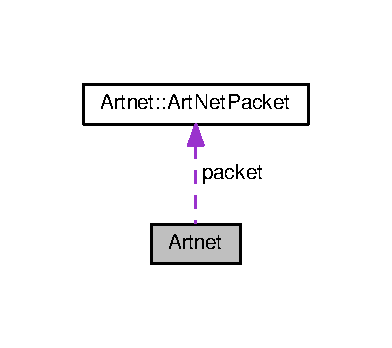
\includegraphics[width=188pt]{classArtnet__coll__graph}
\end{center}
\end{figure}
\subsection*{Classes}
\begin{DoxyCompactItemize}
\item 
struct \hyperlink{structArtnet_1_1ArtNetPacket}{Art\+Net\+Packet}
\begin{DoxyCompactList}\small\item\em An Art-\/\+Net packet. \end{DoxyCompactList}\end{DoxyCompactItemize}
\subsection*{Public Member Functions}
\begin{DoxyCompactItemize}
\item 
\mbox{\Hypertarget{classArtnet_ac3de43f38fbdcc4f737c56c7dd071eb4}\label{classArtnet_ac3de43f38fbdcc4f737c56c7dd071eb4}} 
bool \hyperlink{classArtnet_ac3de43f38fbdcc4f737c56c7dd071eb4}{set\+Channel} (int channel, uint8\+\_\+t value)
\begin{DoxyCompactList}\small\item\em Set a given D\+MX channel to a given value. \end{DoxyCompactList}\item 
\mbox{\Hypertarget{classArtnet_aeb06c6aa3357345140dc9bf6ab024b9e}\label{classArtnet_aeb06c6aa3357345140dc9bf6ab024b9e}} 
void \hyperlink{classArtnet_aeb06c6aa3357345140dc9bf6ab024b9e}{send\+Artnet\+Packet} (std\+::string host, unsigned short port)
\begin{DoxyCompactList}\small\item\em Send an Art-\/\+Net packet to the given address. \end{DoxyCompactList}\end{DoxyCompactItemize}
\subsection*{Private Member Functions}
\begin{DoxyCompactItemize}
\item 
\hyperlink{classSocket}{Socket} $\ast$ \hyperlink{classArtnet_a2ad460313cfce83663c5493ffcebb380}{get\+Socket} ()
\begin{DoxyCompactList}\small\item\em The packet to be sent. \end{DoxyCompactList}\end{DoxyCompactItemize}
\subsection*{Private Attributes}
\begin{DoxyCompactItemize}
\item 
\mbox{\Hypertarget{classArtnet_a9388aaec894174e2d0f39b6f14ea5f50}\label{classArtnet_a9388aaec894174e2d0f39b6f14ea5f50}} 
\hyperlink{structArtnet_1_1ArtNetPacket}{Art\+Net\+Packet} {\bfseries packet}
\end{DoxyCompactItemize}


\subsection{Detailed Description}
A class to send Art-\/\+Net data. 

\subsection{Member Function Documentation}
\mbox{\Hypertarget{classArtnet_a2ad460313cfce83663c5493ffcebb380}\label{classArtnet_a2ad460313cfce83663c5493ffcebb380}} 
\index{Artnet@{Artnet}!get\+Socket@{get\+Socket}}
\index{get\+Socket@{get\+Socket}!Artnet@{Artnet}}
\subsubsection{\texorpdfstring{get\+Socket()}{getSocket()}}
{\footnotesize\ttfamily \hyperlink{classSocket}{Socket}$\ast$ Artnet\+::get\+Socket (\begin{DoxyParamCaption}{ }\end{DoxyParamCaption})\hspace{0.3cm}{\ttfamily [inline]}, {\ttfamily [private]}}



The packet to be sent. 

Get the shared \hyperlink{classSocket}{Socket} 

The documentation for this class was generated from the following files\+:\begin{DoxyCompactItemize}
\item 
src/Artnet.\+hpp\item 
src/Artnet.\+cpp\end{DoxyCompactItemize}

\hypertarget{structArtnet_1_1ArtNetPacket}{}\section{Artnet\+:\+:Art\+Net\+Packet Struct Reference}
\label{structArtnet_1_1ArtNetPacket}\index{Artnet\+::\+Art\+Net\+Packet@{Artnet\+::\+Art\+Net\+Packet}}


An Art-\/\+Net packet.  


\subsection*{Public Attributes}
\begin{DoxyCompactItemize}
\item 
\mbox{\Hypertarget{structArtnet_1_1ArtNetPacket_a6bb1f7f98e789604dc21a15bedc21943}\label{structArtnet_1_1ArtNetPacket_a6bb1f7f98e789604dc21a15bedc21943}} 
uint8\+\_\+t {\bfseries header0} = \textquotesingle{}A\textquotesingle{}
\item 
\mbox{\Hypertarget{structArtnet_1_1ArtNetPacket_a96d5bac6c1acf57aac89ca574d890140}\label{structArtnet_1_1ArtNetPacket_a96d5bac6c1acf57aac89ca574d890140}} 
uint8\+\_\+t {\bfseries header1} = \textquotesingle{}r\textquotesingle{}
\item 
\mbox{\Hypertarget{structArtnet_1_1ArtNetPacket_afd50599c5e6ae3abc58abcd8675438a9}\label{structArtnet_1_1ArtNetPacket_afd50599c5e6ae3abc58abcd8675438a9}} 
uint8\+\_\+t {\bfseries header2} = \textquotesingle{}t\textquotesingle{}
\item 
\mbox{\Hypertarget{structArtnet_1_1ArtNetPacket_a7de8fc6b33c3998967d2e7c4c3b3beda}\label{structArtnet_1_1ArtNetPacket_a7de8fc6b33c3998967d2e7c4c3b3beda}} 
uint8\+\_\+t {\bfseries header3} = \textquotesingle{}-\/\textquotesingle{}
\item 
\mbox{\Hypertarget{structArtnet_1_1ArtNetPacket_a7f54adcee3aaed55e4e89cbcb5141908}\label{structArtnet_1_1ArtNetPacket_a7f54adcee3aaed55e4e89cbcb5141908}} 
uint8\+\_\+t {\bfseries header4} = \textquotesingle{}N\textquotesingle{}
\item 
\mbox{\Hypertarget{structArtnet_1_1ArtNetPacket_a95171885811287edfe8170f6e9cbc3b2}\label{structArtnet_1_1ArtNetPacket_a95171885811287edfe8170f6e9cbc3b2}} 
uint8\+\_\+t {\bfseries header5} = \textquotesingle{}e\textquotesingle{}
\item 
\mbox{\Hypertarget{structArtnet_1_1ArtNetPacket_a40a2523a58975b8bc9e53ecf4e1ff778}\label{structArtnet_1_1ArtNetPacket_a40a2523a58975b8bc9e53ecf4e1ff778}} 
uint8\+\_\+t {\bfseries header6} = \textquotesingle{}t\textquotesingle{}
\item 
\mbox{\Hypertarget{structArtnet_1_1ArtNetPacket_ad4f533e188b56c26caa521dc67e1fcec}\label{structArtnet_1_1ArtNetPacket_ad4f533e188b56c26caa521dc67e1fcec}} 
uint8\+\_\+t {\bfseries header7} = 0
\item 
\mbox{\Hypertarget{structArtnet_1_1ArtNetPacket_a7b97490b76512f800e0f370a2c1317fa}\label{structArtnet_1_1ArtNetPacket_a7b97490b76512f800e0f370a2c1317fa}} 
uint8\+\_\+t {\bfseries opcode\+Lo} = 0x00
\item 
\mbox{\Hypertarget{structArtnet_1_1ArtNetPacket_aa66381b0754cfac0ad68a2d1632ac134}\label{structArtnet_1_1ArtNetPacket_aa66381b0754cfac0ad68a2d1632ac134}} 
uint8\+\_\+t {\bfseries opcode\+Hi} = 0x50
\item 
\mbox{\Hypertarget{structArtnet_1_1ArtNetPacket_af10c66bcb9a4ab7d4f84657241833113}\label{structArtnet_1_1ArtNetPacket_af10c66bcb9a4ab7d4f84657241833113}} 
uint8\+\_\+t {\bfseries version\+Hi} = 00
\item 
\mbox{\Hypertarget{structArtnet_1_1ArtNetPacket_a0a12882d959a2be50206f3b12050d9d0}\label{structArtnet_1_1ArtNetPacket_a0a12882d959a2be50206f3b12050d9d0}} 
uint8\+\_\+t {\bfseries version\+Lo} = 14
\item 
\mbox{\Hypertarget{structArtnet_1_1ArtNetPacket_a78157adb70a494456d9fce018d465116}\label{structArtnet_1_1ArtNetPacket_a78157adb70a494456d9fce018d465116}} 
uint8\+\_\+t {\bfseries sequence} = 1
\item 
\mbox{\Hypertarget{structArtnet_1_1ArtNetPacket_a2f5f981d5841a312a1623b78b114438e}\label{structArtnet_1_1ArtNetPacket_a2f5f981d5841a312a1623b78b114438e}} 
uint8\+\_\+t {\bfseries physical} = 0
\item 
\mbox{\Hypertarget{structArtnet_1_1ArtNetPacket_a78f5d608f6810f7770a59e56d2213fee}\label{structArtnet_1_1ArtNetPacket_a78f5d608f6810f7770a59e56d2213fee}} 
uint8\+\_\+t {\bfseries universe\+Lo} = 0
\item 
\mbox{\Hypertarget{structArtnet_1_1ArtNetPacket_a7a740fd2053a3ef14d268c3a5c5184fb}\label{structArtnet_1_1ArtNetPacket_a7a740fd2053a3ef14d268c3a5c5184fb}} 
uint8\+\_\+t {\bfseries universe\+Hi} = 0
\item 
\mbox{\Hypertarget{structArtnet_1_1ArtNetPacket_aa504b1b621db47a0678655e13d37d426}\label{structArtnet_1_1ArtNetPacket_aa504b1b621db47a0678655e13d37d426}} 
uint8\+\_\+t {\bfseries length\+Hi} = 0x02
\item 
\mbox{\Hypertarget{structArtnet_1_1ArtNetPacket_a2079f7f81420327fc4c369539ab55ecc}\label{structArtnet_1_1ArtNetPacket_a2079f7f81420327fc4c369539ab55ecc}} 
uint8\+\_\+t {\bfseries length\+Lo} = 0x00
\item 
\mbox{\Hypertarget{structArtnet_1_1ArtNetPacket_a08fe2abb7d39d4915dab44ca0d54f641}\label{structArtnet_1_1ArtNetPacket_a08fe2abb7d39d4915dab44ca0d54f641}} 
uint8\+\_\+t {\bfseries data} \mbox{[}512\mbox{]}
\end{DoxyCompactItemize}


\subsection{Detailed Description}
An Art-\/\+Net packet. 

The documentation for this struct was generated from the following file\+:\begin{DoxyCompactItemize}
\item 
src/Artnet.\+hpp\end{DoxyCompactItemize}

\hypertarget{classConfig}{}\section{Config Class Reference}
\label{classConfig}\index{Config@{Config}}


A config parser and writer.  




{\ttfamily \#include $<$Config.\+hpp$>$}

\subsection*{Public Member Functions}
\begin{DoxyCompactItemize}
\item 
\mbox{\Hypertarget{classConfig_aff4607e897113173420e19882796d866}\label{classConfig_aff4607e897113173420e19882796d866}} 
std\+::vector$<$ \hyperlink{structPreset}{Preset} $>$ const  \& \hyperlink{classConfig_aff4607e897113173420e19882796d866}{get\+Presets} ()
\begin{DoxyCompactList}\small\item\em Get the list of presets. \end{DoxyCompactList}\item 
\mbox{\Hypertarget{classConfig_a8cbdb452e8ebd40185783fde637851e4}\label{classConfig_a8cbdb452e8ebd40185783fde637851e4}} 
int \hyperlink{classConfig_a8cbdb452e8ebd40185783fde637851e4}{get\+Skip\+Packet\+Limit} ()
\begin{DoxyCompactList}\small\item\em Get the number of identical packets to be skipped before resending. \end{DoxyCompactList}\item 
\mbox{\Hypertarget{classConfig_ac485e8b97e04fd82ca33c89416fbcce0}\label{classConfig_ac485e8b97e04fd82ca33c89416fbcce0}} 
std\+::chrono\+::milliseconds \hyperlink{classConfig_ac485e8b97e04fd82ca33c89416fbcce0}{get\+Check\+Rate} ()
\begin{DoxyCompactList}\small\item\em Get the time between requests to Virtual\+DJ. \end{DoxyCompactList}\item 
\mbox{\Hypertarget{classConfig_a12421ddabec031b3d724d377fc920c8d}\label{classConfig_a12421ddabec031b3d724d377fc920c8d}} 
\hyperlink{classConfig_a12421ddabec031b3d724d377fc920c8d}{Config} (std\+::string config\+Path\+T\+MP)
\begin{DoxyCompactList}\small\item\em Constuct a config parser for the given config file. \end{DoxyCompactList}\item 
\mbox{\Hypertarget{classConfig_a38d923d7d9553c2e92559c599937100b}\label{classConfig_a38d923d7d9553c2e92559c599937100b}} 
void \hyperlink{classConfig_a38d923d7d9553c2e92559c599937100b}{load\+Config} ()
\begin{DoxyCompactList}\small\item\em Load the config file. \end{DoxyCompactList}\item 
\mbox{\Hypertarget{classConfig_a64000eb3f2292cba44278cec34fc076d}\label{classConfig_a64000eb3f2292cba44278cec34fc076d}} 
void \hyperlink{classConfig_a64000eb3f2292cba44278cec34fc076d}{save\+Config} ()
\begin{DoxyCompactList}\small\item\em Save the config file. \end{DoxyCompactList}\end{DoxyCompactItemize}
\subsection*{Public Attributes}
\begin{DoxyCompactItemize}
\item 
\mbox{\Hypertarget{classConfig_ada2efbde15130b44645f383ed71894ae}\label{classConfig_ada2efbde15130b44645f383ed71894ae}} 
std\+::string \hyperlink{classConfig_ada2efbde15130b44645f383ed71894ae}{channel\+Commands} \mbox{[}512\mbox{]}
\begin{DoxyCompactList}\small\item\em The list of commands to be sent to Virtual\+DJ. \end{DoxyCompactList}\item 
\mbox{\Hypertarget{classConfig_aff7a38d3fada71d2d0aa7e1b01c43ea7}\label{classConfig_aff7a38d3fada71d2d0aa7e1b01c43ea7}} 
std\+::string \hyperlink{classConfig_aff7a38d3fada71d2d0aa7e1b01c43ea7}{host} = \char`\"{}127.\+0.\+0.\+1\char`\"{}
\begin{DoxyCompactList}\small\item\em The host to which the Art-\/\+Net data should be sent. \end{DoxyCompactList}\item 
\mbox{\Hypertarget{classConfig_a5e0403fc897ee2ac5571ee45c6803d3e}\label{classConfig_a5e0403fc897ee2ac5571ee45c6803d3e}} 
unsigned short \hyperlink{classConfig_a5e0403fc897ee2ac5571ee45c6803d3e}{port} = 0x1936
\begin{DoxyCompactList}\small\item\em The port on which the Art-\/\+Net data should be sent. \end{DoxyCompactList}\end{DoxyCompactItemize}
\subsection*{Private Member Functions}
\begin{DoxyCompactItemize}
\item 
\mbox{\Hypertarget{classConfig_ab3f3b04d3ab2602141212c1af509b808}\label{classConfig_ab3f3b04d3ab2602141212c1af509b808}} 
void \hyperlink{classConfig_ab3f3b04d3ab2602141212c1af509b808}{load\+Preset\+Presets} ()
\begin{DoxyCompactList}\small\item\em Load the pre compiled presets. \end{DoxyCompactList}\item 
\mbox{\Hypertarget{classConfig_ad05fb468c16ec451652abb2de179caf5}\label{classConfig_ad05fb468c16ec451652abb2de179caf5}} 
void \hyperlink{classConfig_ad05fb468c16ec451652abb2de179caf5}{parse\+Presets\+Stream} (std\+::istream \&fin)
\begin{DoxyCompactList}\small\item\em Parse the given stream for presets. \end{DoxyCompactList}\item 
void \hyperlink{classConfig_a9f578681efe13ea4c4baca735f6b3c6e}{parse\+Presets\+Line} (std\+::string line)
\begin{DoxyCompactList}\small\item\em Parse the given string for a preset. \end{DoxyCompactList}\item 
\mbox{\Hypertarget{classConfig_a6c2a4d8a853cbcc51825d3cb0c96ff61}\label{classConfig_a6c2a4d8a853cbcc51825d3cb0c96ff61}} 
void \hyperlink{classConfig_a6c2a4d8a853cbcc51825d3cb0c96ff61}{parse\+Config\+File} (std\+::ifstream \&fin)
\begin{DoxyCompactList}\small\item\em Parse the given file for presets. \end{DoxyCompactList}\item 
void \hyperlink{classConfig_a9a85fd4fb07775bccf974a83645159e2}{parse\+Config\+Line} (std\+::string line)
\begin{DoxyCompactList}\small\item\em Parse the given string for a config command. \end{DoxyCompactList}\end{DoxyCompactItemize}
\subsection*{Private Attributes}
\begin{DoxyCompactItemize}
\item 
\mbox{\Hypertarget{classConfig_aa82482a705c93a00da195e3f9f974b23}\label{classConfig_aa82482a705c93a00da195e3f9f974b23}} 
std\+::string \hyperlink{classConfig_aa82482a705c93a00da195e3f9f974b23}{config\+Path}
\begin{DoxyCompactList}\small\item\em The config file to parse. \end{DoxyCompactList}\item 
\mbox{\Hypertarget{classConfig_a28f392a11a7cd755cd7493b25c8e89d0}\label{classConfig_a28f392a11a7cd755cd7493b25c8e89d0}} 
std\+::vector$<$ \hyperlink{structPreset}{Preset} $>$ \hyperlink{classConfig_a28f392a11a7cd755cd7493b25c8e89d0}{presets}
\begin{DoxyCompactList}\small\item\em The list of presets. \end{DoxyCompactList}\item 
std\+::set$<$ std\+::string $>$ \hyperlink{classConfig_a02be73634e4b7debd0551a360dac9503}{loaded\+Config\+Paths}
\begin{DoxyCompactList}\small\item\em The set of config files already parsed. \end{DoxyCompactList}\item 
\mbox{\Hypertarget{classConfig_adb31288f02cd583f05a37faf787c480b}\label{classConfig_adb31288f02cd583f05a37faf787c480b}} 
int \hyperlink{classConfig_adb31288f02cd583f05a37faf787c480b}{skip\+Packet\+Limit}
\begin{DoxyCompactList}\small\item\em The number of identical packets to be skipped before resending. \end{DoxyCompactList}\item 
\mbox{\Hypertarget{classConfig_a7c4280b4a4c2f24cd98518f5d9757d2e}\label{classConfig_a7c4280b4a4c2f24cd98518f5d9757d2e}} 
std\+::chrono\+::milliseconds \hyperlink{classConfig_a7c4280b4a4c2f24cd98518f5d9757d2e}{check\+Rate} = std\+::chrono\+::milliseconds(10)
\begin{DoxyCompactList}\small\item\em The time between requests to Virtual\+DJ. \end{DoxyCompactList}\end{DoxyCompactItemize}


\subsection{Detailed Description}
A config parser and writer. 

\subsection{Member Function Documentation}
\mbox{\Hypertarget{classConfig_a9a85fd4fb07775bccf974a83645159e2}\label{classConfig_a9a85fd4fb07775bccf974a83645159e2}} 
\index{Config@{Config}!parse\+Config\+Line@{parse\+Config\+Line}}
\index{parse\+Config\+Line@{parse\+Config\+Line}!Config@{Config}}
\subsubsection{\texorpdfstring{parse\+Config\+Line()}{parseConfigLine()}}
{\footnotesize\ttfamily void Config\+::parse\+Config\+Line (\begin{DoxyParamCaption}\item[{std\+::string}]{line }\end{DoxyParamCaption})\hspace{0.3cm}{\ttfamily [private]}}



Parse the given string for a config command. 

A $\sim$ should be used between the channel number and the command. \mbox{\Hypertarget{classConfig_a9f578681efe13ea4c4baca735f6b3c6e}\label{classConfig_a9f578681efe13ea4c4baca735f6b3c6e}} 
\index{Config@{Config}!parse\+Presets\+Line@{parse\+Presets\+Line}}
\index{parse\+Presets\+Line@{parse\+Presets\+Line}!Config@{Config}}
\subsubsection{\texorpdfstring{parse\+Presets\+Line()}{parsePresetsLine()}}
{\footnotesize\ttfamily void Config\+::parse\+Presets\+Line (\begin{DoxyParamCaption}\item[{std\+::string}]{line }\end{DoxyParamCaption})\hspace{0.3cm}{\ttfamily [private]}}



Parse the given string for a preset. 

A $\sim$ should be used between the name and the command. 

\subsection{Member Data Documentation}
\mbox{\Hypertarget{classConfig_a02be73634e4b7debd0551a360dac9503}\label{classConfig_a02be73634e4b7debd0551a360dac9503}} 
\index{Config@{Config}!loaded\+Config\+Paths@{loaded\+Config\+Paths}}
\index{loaded\+Config\+Paths@{loaded\+Config\+Paths}!Config@{Config}}
\subsubsection{\texorpdfstring{loaded\+Config\+Paths}{loadedConfigPaths}}
{\footnotesize\ttfamily std\+::set$<$std\+::string$>$ Config\+::loaded\+Config\+Paths\hspace{0.3cm}{\ttfamily [private]}}



The set of config files already parsed. 

This is used to prevent an infinite loop. 

The documentation for this class was generated from the following files\+:\begin{DoxyCompactItemize}
\item 
src/\hyperlink{Config_8hpp}{Config.\+hpp}\item 
src/Config.\+cpp\end{DoxyCompactItemize}

\hypertarget{interfaceConfigEditMenu}{}\section{Config\+Edit\+Menu Class Reference}
\label{interfaceConfigEditMenu}\index{Config\+Edit\+Menu@{Config\+Edit\+Menu}}


Inheritance diagram for Config\+Edit\+Menu\+:
\nopagebreak
\begin{figure}[H]
\begin{center}
\leavevmode
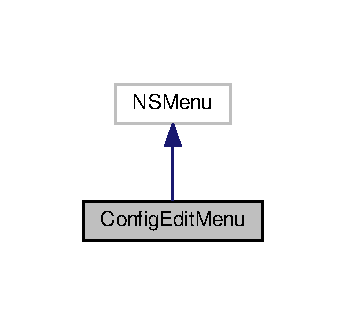
\includegraphics[width=166pt]{interfaceConfigEditMenu__inherit__graph}
\end{center}
\end{figure}


Collaboration diagram for Config\+Edit\+Menu\+:
\nopagebreak
\begin{figure}[H]
\begin{center}
\leavevmode
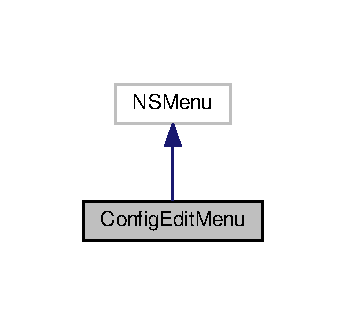
\includegraphics[width=166pt]{interfaceConfigEditMenu__coll__graph}
\end{center}
\end{figure}
\subsection*{Instance Methods}
\begin{DoxyCompactItemize}
\item 
(id) -\/ {\bfseries init\+With\+Undo\+Manager\+:view\+Controller\+:}
\item 
\mbox{\Hypertarget{interfaceConfigEditMenu_a1599e444ad49a8a8f8239d573377a8a8}\label{interfaceConfigEditMenu_a1599e444ad49a8a8f8239d573377a8a8}} 
(void) -\/ {\bfseries copy\+Row}
\item 
\mbox{\Hypertarget{interfaceConfigEditMenu_a9350af3e1ce284e899a35f472ce28333}\label{interfaceConfigEditMenu_a9350af3e1ce284e899a35f472ce28333}} 
(void) -\/ {\bfseries paste\+Row}
\item 
\mbox{\Hypertarget{interfaceConfigEditMenu_a0d71c491814ce8616568b11cb1a931ac}\label{interfaceConfigEditMenu_a0d71c491814ce8616568b11cb1a931ac}} 
(void) -\/ {\bfseries delete\+Row}
\end{DoxyCompactItemize}


\subsection{Method Documentation}
\mbox{\Hypertarget{interfaceConfigEditMenu_a4e4d50ce26c275b2ab20f656d5886dc4}\label{interfaceConfigEditMenu_a4e4d50ce26c275b2ab20f656d5886dc4}} 
\index{Config\+Edit\+Menu@{Config\+Edit\+Menu}!init\+With\+Undo\+Manager\+:view\+Controller\+:@{init\+With\+Undo\+Manager\+:view\+Controller\+:}}
\index{init\+With\+Undo\+Manager\+:view\+Controller\+:@{init\+With\+Undo\+Manager\+:view\+Controller\+:}!Config\+Edit\+Menu@{Config\+Edit\+Menu}}
\subsubsection{\texorpdfstring{init\+With\+Undo\+Manager\+:view\+Controller\+:()}{initWithUndoManager:viewController:()}}
{\footnotesize\ttfamily -\/ (id) init\+With\+Undo\+Manager\+: \begin{DoxyParamCaption}\item[{(N\+S\+Undo\+Manager$\ast$)}]{undo\+Manager }\item[{viewController:(\hyperlink{interfaceConfigViewController}{Config\+View\+Controller}$\ast$)}]{view\+Controller\+T\+MP }\end{DoxyParamCaption}}

{\bfseries Initial value\+:}
\begin{DoxyCode}
\{
    \hyperlink{interfaceConfigViewController}{ConfigViewController}* viewController
\end{DoxyCode}


The documentation for this class was generated from the following files\+:\begin{DoxyCompactItemize}
\item 
src/Config\+Mac\+Edit\+Menu.\+h\item 
src/Config\+Mac\+Edit\+Menu.\+mm\end{DoxyCompactItemize}

\hypertarget{interfaceConfigIpAddress}{}\section{Config\+Ip\+Address Class Reference}
\label{interfaceConfigIpAddress}\index{Config\+Ip\+Address@{Config\+Ip\+Address}}


Inheritance diagram for Config\+Ip\+Address\+:
\nopagebreak
\begin{figure}[H]
\begin{center}
\leavevmode
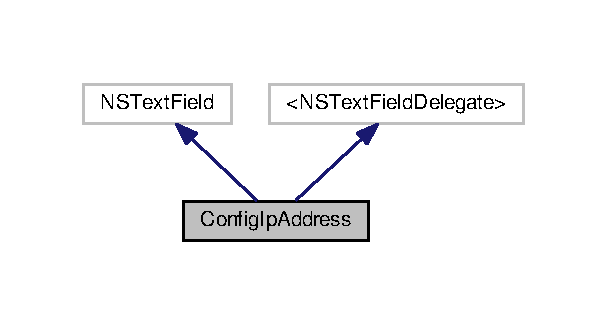
\includegraphics[width=292pt]{interfaceConfigIpAddress__inherit__graph}
\end{center}
\end{figure}


Collaboration diagram for Config\+Ip\+Address\+:
\nopagebreak
\begin{figure}[H]
\begin{center}
\leavevmode
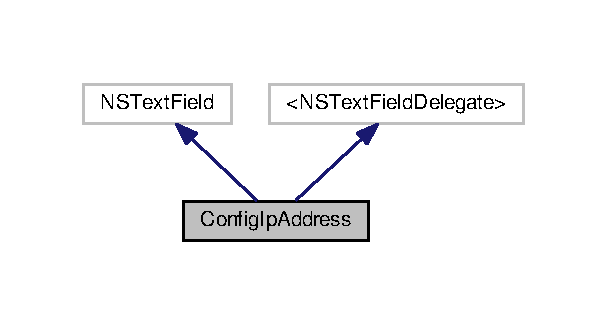
\includegraphics[width=292pt]{interfaceConfigIpAddress__coll__graph}
\end{center}
\end{figure}
\subsection*{Instance Methods}
\begin{DoxyCompactItemize}
\item 
(id) -\/ {\bfseries init\+With\+Frame\+:\+V\+D\+Jartnet\+:}
\item 
\mbox{\Hypertarget{interfaceConfigIpAddress_a62f80031eea3a4d441b16daeb9ee0e4f}\label{interfaceConfigIpAddress_a62f80031eea3a4d441b16daeb9ee0e4f}} 
(B\+O\+OL) -\/ {\bfseries control\+:text\+Should\+End\+Editing\+:}
\end{DoxyCompactItemize}


\subsection{Method Documentation}
\mbox{\Hypertarget{interfaceConfigIpAddress_aca31bc2897a8952983169dca717fff29}\label{interfaceConfigIpAddress_aca31bc2897a8952983169dca717fff29}} 
\index{Config\+Ip\+Address@{Config\+Ip\+Address}!init\+With\+Frame\+:\+V\+D\+Jartnet\+:@{init\+With\+Frame\+:\+V\+D\+Jartnet\+:}}
\index{init\+With\+Frame\+:\+V\+D\+Jartnet\+:@{init\+With\+Frame\+:\+V\+D\+Jartnet\+:}!Config\+Ip\+Address@{Config\+Ip\+Address}}
\subsubsection{\texorpdfstring{init\+With\+Frame\+:\+V\+D\+Jartnet\+:()}{initWithFrame:VDJartnet:()}}
{\footnotesize\ttfamily -\/ (id) init\+With\+Frame\+: \begin{DoxyParamCaption}\item[{(C\+G\+Rect)}]{frame }\item[{VDJartnet:(\hyperlink{classCVDJartnet}{C\+V\+D\+Jartnet}$\ast$)}]{vdj\+Artnet\+T\+MP }\end{DoxyParamCaption}}

{\bfseries Initial value\+:}
\begin{DoxyCode}
\{
    \hyperlink{classCVDJartnet}{CVDJartnet}* vdjArtnet
\end{DoxyCode}


The documentation for this class was generated from the following files\+:\begin{DoxyCompactItemize}
\item 
src/Config\+Mac\+Ip\+Address.\+h\item 
src/Config\+Mac\+Ip\+Address.\+mm\end{DoxyCompactItemize}

\hypertarget{interfaceConfigIpPort}{}\section{Config\+Ip\+Port Class Reference}
\label{interfaceConfigIpPort}\index{Config\+Ip\+Port@{Config\+Ip\+Port}}


Inheritance diagram for Config\+Ip\+Port\+:
\nopagebreak
\begin{figure}[H]
\begin{center}
\leavevmode
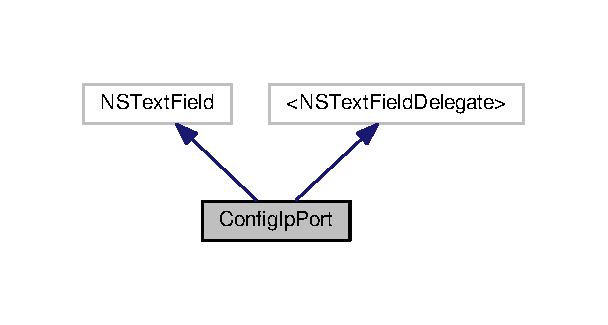
\includegraphics[width=292pt]{interfaceConfigIpPort__inherit__graph}
\end{center}
\end{figure}


Collaboration diagram for Config\+Ip\+Port\+:
\nopagebreak
\begin{figure}[H]
\begin{center}
\leavevmode
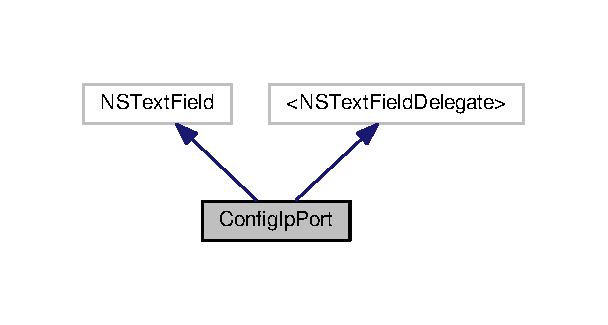
\includegraphics[width=292pt]{interfaceConfigIpPort__coll__graph}
\end{center}
\end{figure}
\subsection*{Instance Methods}
\begin{DoxyCompactItemize}
\item 
(id) -\/ {\bfseries init\+With\+Frame\+:\+V\+D\+Jartnet\+:}
\item 
\mbox{\Hypertarget{interfaceConfigIpPort_a06af11278d360cb589b1a7770ac21981}\label{interfaceConfigIpPort_a06af11278d360cb589b1a7770ac21981}} 
(B\+O\+OL) -\/ {\bfseries control\+:text\+Should\+End\+Editing\+:}
\end{DoxyCompactItemize}


\subsection{Method Documentation}
\mbox{\Hypertarget{interfaceConfigIpPort_a0ec5c58834c67ee1271aa7f1a83239e9}\label{interfaceConfigIpPort_a0ec5c58834c67ee1271aa7f1a83239e9}} 
\index{Config\+Ip\+Port@{Config\+Ip\+Port}!init\+With\+Frame\+:\+V\+D\+Jartnet\+:@{init\+With\+Frame\+:\+V\+D\+Jartnet\+:}}
\index{init\+With\+Frame\+:\+V\+D\+Jartnet\+:@{init\+With\+Frame\+:\+V\+D\+Jartnet\+:}!Config\+Ip\+Port@{Config\+Ip\+Port}}
\subsubsection{\texorpdfstring{init\+With\+Frame\+:\+V\+D\+Jartnet\+:()}{initWithFrame:VDJartnet:()}}
{\footnotesize\ttfamily -\/ (id) init\+With\+Frame\+: \begin{DoxyParamCaption}\item[{(C\+G\+Rect)}]{frame }\item[{VDJartnet:(\hyperlink{classCVDJartnet}{C\+V\+D\+Jartnet}$\ast$)}]{vdj\+Artnet\+T\+MP }\end{DoxyParamCaption}}

{\bfseries Initial value\+:}
\begin{DoxyCode}
\{
    \hyperlink{classCVDJartnet}{CVDJartnet}* vdjArtnet
\end{DoxyCode}


The documentation for this class was generated from the following files\+:\begin{DoxyCompactItemize}
\item 
src/Config\+Mac\+Ip\+Port.\+h\item 
src/Config\+Mac\+Ip\+Port.\+mm\end{DoxyCompactItemize}

\hypertarget{interfaceConfigPresetDataSource}{}\section{Config\+Preset\+Data\+Source Class Reference}
\label{interfaceConfigPresetDataSource}\index{Config\+Preset\+Data\+Source@{Config\+Preset\+Data\+Source}}


Inheritance diagram for Config\+Preset\+Data\+Source\+:
\nopagebreak
\begin{figure}[H]
\begin{center}
\leavevmode
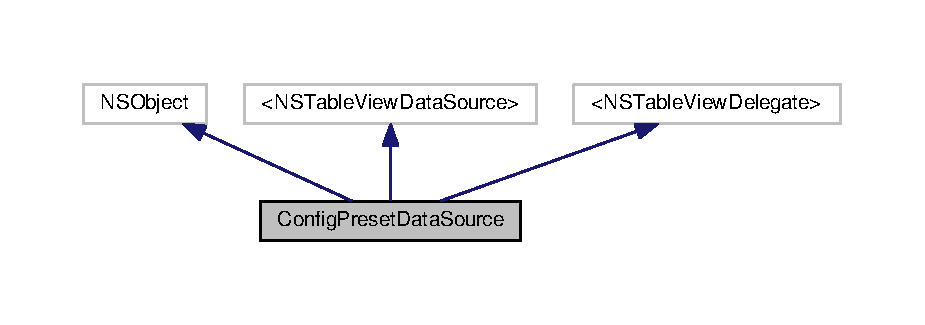
\includegraphics[width=350pt]{interfaceConfigPresetDataSource__inherit__graph}
\end{center}
\end{figure}


Collaboration diagram for Config\+Preset\+Data\+Source\+:
\nopagebreak
\begin{figure}[H]
\begin{center}
\leavevmode
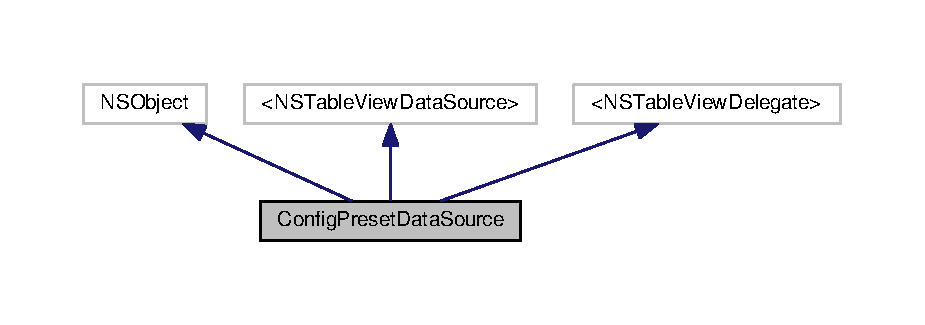
\includegraphics[width=350pt]{interfaceConfigPresetDataSource__coll__graph}
\end{center}
\end{figure}
\subsection*{Instance Methods}
\begin{DoxyCompactItemize}
\item 
(id) -\/ {\bfseries init\+With\+V\+D\+Jartnet\+:}
\item 
\mbox{\Hypertarget{interfaceConfigPresetDataSource_a9b2f2c389b66cbb8b0d8ead92c89dfbe}\label{interfaceConfigPresetDataSource_a9b2f2c389b66cbb8b0d8ead92c89dfbe}} 
(N\+S\+Integer) -\/ {\bfseries number\+Of\+Rows\+In\+Table\+View\+:}
\item 
\mbox{\Hypertarget{interfaceConfigPresetDataSource_a016a352e7ee71c2a1b8672ed6c72de6e}\label{interfaceConfigPresetDataSource_a016a352e7ee71c2a1b8672ed6c72de6e}} 
(id) -\/ {\bfseries table\+View\+:object\+Value\+For\+Table\+Column\+:row\+:}
\item 
\mbox{\Hypertarget{interfaceConfigPresetDataSource_a98f7fe5b7e450ae9a584a7391795d330}\label{interfaceConfigPresetDataSource_a98f7fe5b7e450ae9a584a7391795d330}} 
(B\+O\+OL) -\/ {\bfseries table\+View\+:write\+Rows\+With\+Indexes\+:to\+Pasteboard\+:}
\end{DoxyCompactItemize}


\subsection{Method Documentation}
\mbox{\Hypertarget{interfaceConfigPresetDataSource_aa9dd674164d07d7f57974cb9242a9a5c}\label{interfaceConfigPresetDataSource_aa9dd674164d07d7f57974cb9242a9a5c}} 
\index{Config\+Preset\+Data\+Source@{Config\+Preset\+Data\+Source}!init\+With\+V\+D\+Jartnet\+:@{init\+With\+V\+D\+Jartnet\+:}}
\index{init\+With\+V\+D\+Jartnet\+:@{init\+With\+V\+D\+Jartnet\+:}!Config\+Preset\+Data\+Source@{Config\+Preset\+Data\+Source}}
\subsubsection{\texorpdfstring{init\+With\+V\+D\+Jartnet\+:()}{initWithVDJartnet:()}}
{\footnotesize\ttfamily -\/ (id) init\+With\+V\+D\+Jartnet\+: \begin{DoxyParamCaption}\item[{(\hyperlink{classCVDJartnet}{C\+V\+D\+Jartnet}$\ast$)}]{vdj\+Artnet\+T\+MP }\end{DoxyParamCaption}}

{\bfseries Initial value\+:}
\begin{DoxyCode}
\{
    \hyperlink{classCVDJartnet}{CVDJartnet}* vdjArtnet
\end{DoxyCode}


The documentation for this class was generated from the following files\+:\begin{DoxyCompactItemize}
\item 
src/Config\+Mac\+Preset\+Data\+Source.\+h\item 
src/Config\+Mac\+Preset\+Data\+Source.\+mm\end{DoxyCompactItemize}

\hypertarget{interfaceConfigPresetWindow}{}\section{Config\+Preset\+Window Class Reference}
\label{interfaceConfigPresetWindow}\index{Config\+Preset\+Window@{Config\+Preset\+Window}}


Inheritance diagram for Config\+Preset\+Window\+:
\nopagebreak
\begin{figure}[H]
\begin{center}
\leavevmode
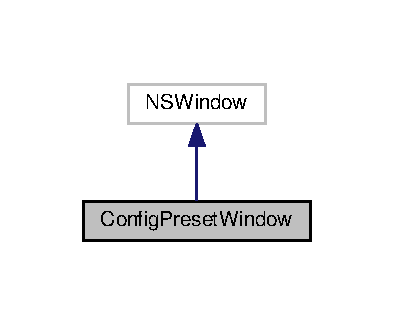
\includegraphics[width=189pt]{interfaceConfigPresetWindow__inherit__graph}
\end{center}
\end{figure}


Collaboration diagram for Config\+Preset\+Window\+:
\nopagebreak
\begin{figure}[H]
\begin{center}
\leavevmode
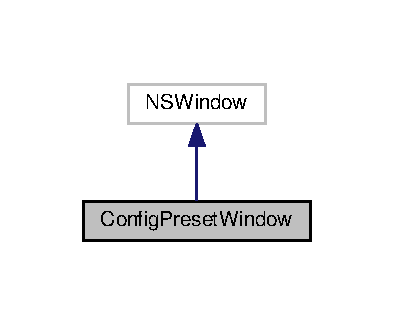
\includegraphics[width=189pt]{interfaceConfigPresetWindow__coll__graph}
\end{center}
\end{figure}
\subsection*{Instance Methods}
\begin{DoxyCompactItemize}
\item 
\mbox{\Hypertarget{interfaceConfigPresetWindow_ad103b27046e919b6721f1407ca513e72}\label{interfaceConfigPresetWindow_ad103b27046e919b6721f1407ca513e72}} 
(id) -\/ {\bfseries init\+With\+V\+D\+Jartnet\+:}
\end{DoxyCompactItemize}


The documentation for this class was generated from the following files\+:\begin{DoxyCompactItemize}
\item 
src/Config\+Mac\+Preset\+Window.\+h\item 
src/Config\+Mac\+Preset\+Window.\+mm\end{DoxyCompactItemize}

\hypertarget{interfaceConfigTableView}{}\section{Config\+Table\+View Class Reference}
\label{interfaceConfigTableView}\index{Config\+Table\+View@{Config\+Table\+View}}


Inheritance diagram for Config\+Table\+View\+:
\nopagebreak
\begin{figure}[H]
\begin{center}
\leavevmode
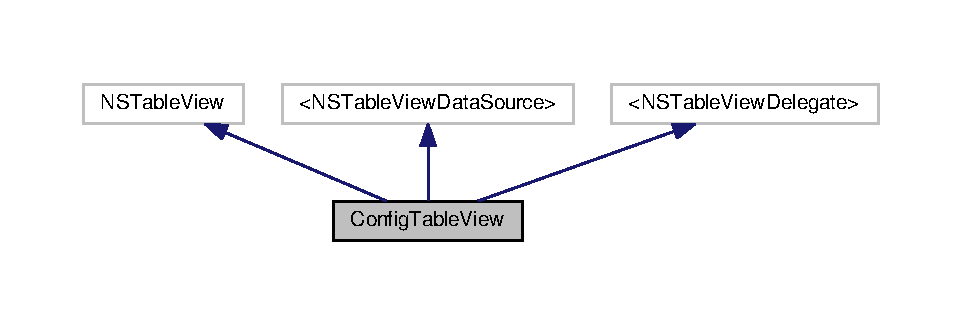
\includegraphics[width=350pt]{interfaceConfigTableView__inherit__graph}
\end{center}
\end{figure}


Collaboration diagram for Config\+Table\+View\+:
\nopagebreak
\begin{figure}[H]
\begin{center}
\leavevmode
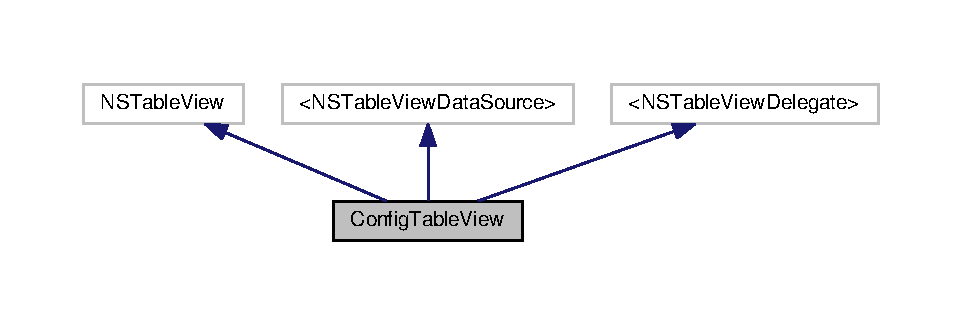
\includegraphics[width=350pt]{interfaceConfigTableView__coll__graph}
\end{center}
\end{figure}
\subsection*{Instance Methods}
\begin{DoxyCompactItemize}
\item 
(id) -\/ {\bfseries init\+With\+V\+D\+Jartnet\+:}
\item 
\mbox{\Hypertarget{interfaceConfigTableView_ad96b218833fd0366e439418c67c83c72}\label{interfaceConfigTableView_ad96b218833fd0366e439418c67c83c72}} 
(N\+S\+Drag\+Operation) -\/ {\bfseries dragging\+Source\+Operation\+Mask\+For\+Local\+:}
\item 
\mbox{\Hypertarget{interfaceConfigTableView_a2c830f2f6a595e4cbfa68f379ceab89a}\label{interfaceConfigTableView_a2c830f2f6a595e4cbfa68f379ceab89a}} 
(N\+S\+Integer) -\/ {\bfseries number\+Of\+Rows\+In\+Table\+View\+:}
\item 
\mbox{\Hypertarget{interfaceConfigTableView_a3c4200b20189a542326a184a4b8cea96}\label{interfaceConfigTableView_a3c4200b20189a542326a184a4b8cea96}} 
(id) -\/ {\bfseries table\+View\+:object\+Value\+For\+Table\+Column\+:row\+:}
\item 
\mbox{\Hypertarget{interfaceConfigTableView_a51b57ad7701c1c71dc1859b10c4861a1}\label{interfaceConfigTableView_a51b57ad7701c1c71dc1859b10c4861a1}} 
(void) -\/ {\bfseries table\+View\+:set\+Object\+Value\+:for\+Table\+Column\+:row\+:}
\item 
\mbox{\Hypertarget{interfaceConfigTableView_a1f66d901e0dd655d5306c2de940d6cb4}\label{interfaceConfigTableView_a1f66d901e0dd655d5306c2de940d6cb4}} 
(B\+O\+OL) -\/ {\bfseries table\+View\+:write\+Rows\+With\+Indexes\+:to\+Pasteboard\+:}
\item 
\mbox{\Hypertarget{interfaceConfigTableView_aa575e068650bc14812b96d14b09c9d72}\label{interfaceConfigTableView_aa575e068650bc14812b96d14b09c9d72}} 
(N\+S\+Drag\+Operation) -\/ {\bfseries table\+View\+:validate\+Drop\+:proposed\+Row\+:proposed\+Drop\+Operation\+:}
\item 
\mbox{\Hypertarget{interfaceConfigTableView_a2851d54065f8df88edd3cd382f077df9}\label{interfaceConfigTableView_a2851d54065f8df88edd3cd382f077df9}} 
(B\+O\+OL) -\/ {\bfseries table\+View\+:accept\+Drop\+:row\+:drop\+Operation\+:}
\end{DoxyCompactItemize}


\subsection{Method Documentation}
\mbox{\Hypertarget{interfaceConfigTableView_a5366e28ba30cf4b1b488457b70101444}\label{interfaceConfigTableView_a5366e28ba30cf4b1b488457b70101444}} 
\index{Config\+Table\+View@{Config\+Table\+View}!init\+With\+V\+D\+Jartnet\+:@{init\+With\+V\+D\+Jartnet\+:}}
\index{init\+With\+V\+D\+Jartnet\+:@{init\+With\+V\+D\+Jartnet\+:}!Config\+Table\+View@{Config\+Table\+View}}
\subsubsection{\texorpdfstring{init\+With\+V\+D\+Jartnet\+:()}{initWithVDJartnet:()}}
{\footnotesize\ttfamily -\/ (id) init\+With\+V\+D\+Jartnet\+: \begin{DoxyParamCaption}\item[{(\hyperlink{classCVDJartnet}{C\+V\+D\+Jartnet}$\ast$)}]{vdj\+Artnet\+T\+MP }\end{DoxyParamCaption}}

{\bfseries Initial value\+:}
\begin{DoxyCode}
\{
    \hyperlink{classCVDJartnet}{CVDJartnet}* vdjArtnet
\end{DoxyCode}


The documentation for this class was generated from the following files\+:\begin{DoxyCompactItemize}
\item 
src/Config\+Mac\+Table\+View.\+h\item 
src/Config\+Mac\+Table\+View.\+mm\end{DoxyCompactItemize}

\hypertarget{interfaceConfigTool}{}\section{Config\+Tool Class Reference}
\label{interfaceConfigTool}\index{Config\+Tool@{Config\+Tool}}


Inheritance diagram for Config\+Tool\+:
\nopagebreak
\begin{figure}[H]
\begin{center}
\leavevmode
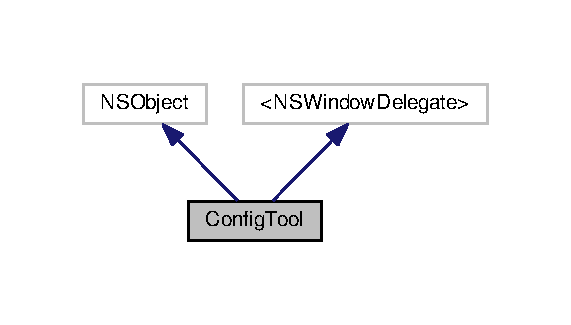
\includegraphics[width=274pt]{interfaceConfigTool__inherit__graph}
\end{center}
\end{figure}


Collaboration diagram for Config\+Tool\+:
\nopagebreak
\begin{figure}[H]
\begin{center}
\leavevmode
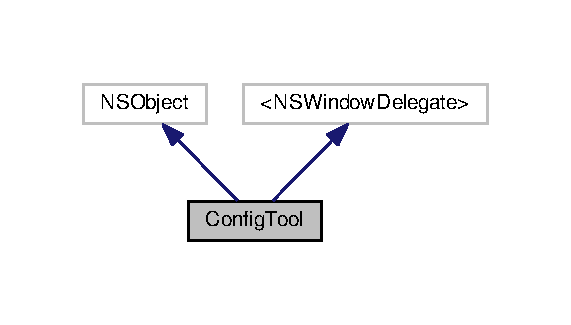
\includegraphics[width=274pt]{interfaceConfigTool__coll__graph}
\end{center}
\end{figure}
\subsection*{Instance Methods}
\begin{DoxyCompactItemize}
\item 
\mbox{\Hypertarget{interfaceConfigTool_a9909af259d86d8b9b32440b6ef1a14bd}\label{interfaceConfigTool_a9909af259d86d8b9b32440b6ef1a14bd}} 
(id) -\/ {\bfseries init\+With\+V\+D\+Jartnet\+:}
\item 
\mbox{\Hypertarget{interfaceConfigTool_af3f58f91aca9a9c58647b8de7b49db00}\label{interfaceConfigTool_af3f58f91aca9a9c58647b8de7b49db00}} 
(void) -\/ {\bfseries dealloc}
\end{DoxyCompactItemize}


The documentation for this class was generated from the following files\+:\begin{DoxyCompactItemize}
\item 
src/Config\+Mac.\+h\item 
src/Config\+Mac.\+mm\end{DoxyCompactItemize}

\hypertarget{interfaceConfigViewController}{}\section{Config\+View\+Controller Class Reference}
\label{interfaceConfigViewController}\index{Config\+View\+Controller@{Config\+View\+Controller}}


Inheritance diagram for Config\+View\+Controller\+:
\nopagebreak
\begin{figure}[H]
\begin{center}
\leavevmode
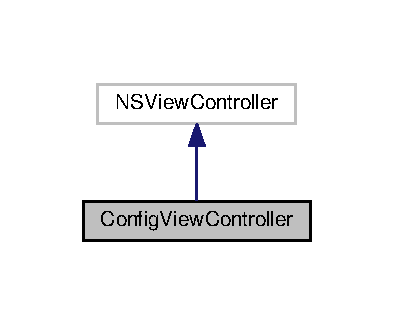
\includegraphics[width=189pt]{interfaceConfigViewController__inherit__graph}
\end{center}
\end{figure}


Collaboration diagram for Config\+View\+Controller\+:
\nopagebreak
\begin{figure}[H]
\begin{center}
\leavevmode
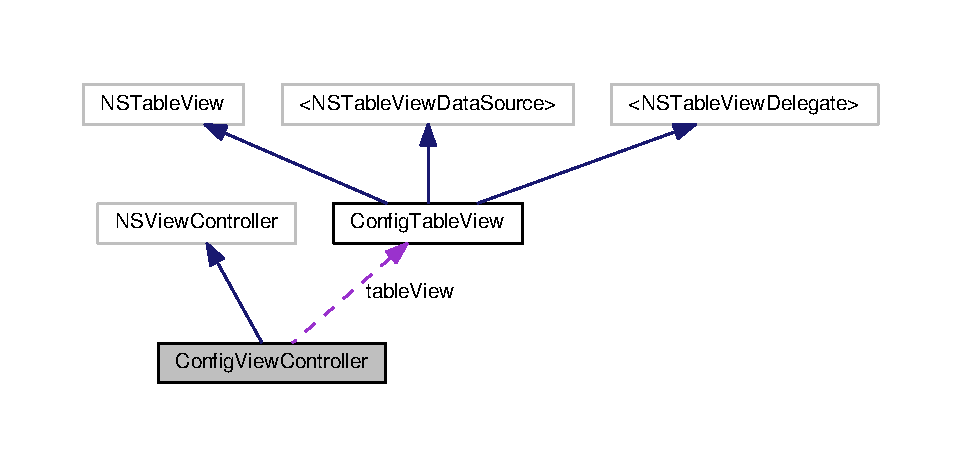
\includegraphics[width=350pt]{interfaceConfigViewController__coll__graph}
\end{center}
\end{figure}
\subsection*{Instance Methods}
\begin{DoxyCompactItemize}
\item 
\mbox{\Hypertarget{interfaceConfigViewController_aa8041471bf58ccce553995071fe913bf}\label{interfaceConfigViewController_aa8041471bf58ccce553995071fe913bf}} 
(id) -\/ {\bfseries init\+With\+V\+D\+Jartnet\+:}
\item 
\mbox{\Hypertarget{interfaceConfigViewController_ab844ba3ae117280d72070390cdf93571}\label{interfaceConfigViewController_ab844ba3ae117280d72070390cdf93571}} 
(void) -\/ {\bfseries load\+View}
\item 
\mbox{\Hypertarget{interfaceConfigViewController_ade565be573576edc51a964c787ab9709}\label{interfaceConfigViewController_ade565be573576edc51a964c787ab9709}} 
(void) -\/ {\bfseries view\+Did\+Layout}
\end{DoxyCompactItemize}
\subsection*{Properties}
\begin{DoxyCompactItemize}
\item 
\mbox{\Hypertarget{interfaceConfigViewController_a70244832aa26bf33937bba95badc35ae}\label{interfaceConfigViewController_a70244832aa26bf33937bba95badc35ae}} 
\hyperlink{interfaceConfigTableView}{Config\+Table\+View} $\ast$ {\bfseries table\+View}
\end{DoxyCompactItemize}


The documentation for this class was generated from the following files\+:\begin{DoxyCompactItemize}
\item 
src/Config\+Mac\+View\+Controller.\+h\item 
src/Config\+Mac\+View\+Controller.\+mm\end{DoxyCompactItemize}

\hypertarget{interfaceConfigWindow}{}\section{Config\+Window Class Reference}
\label{interfaceConfigWindow}\index{Config\+Window@{Config\+Window}}


Inheritance diagram for Config\+Window\+:
\nopagebreak
\begin{figure}[H]
\begin{center}
\leavevmode
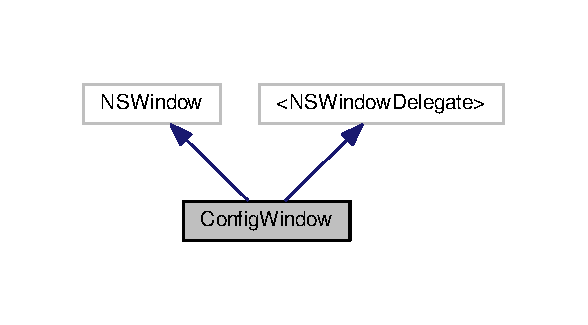
\includegraphics[width=282pt]{interfaceConfigWindow__inherit__graph}
\end{center}
\end{figure}


Collaboration diagram for Config\+Window\+:
\nopagebreak
\begin{figure}[H]
\begin{center}
\leavevmode
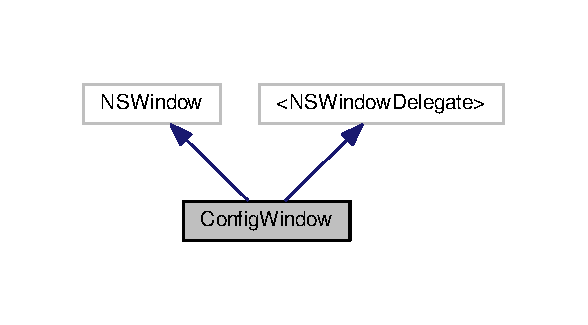
\includegraphics[width=282pt]{interfaceConfigWindow__coll__graph}
\end{center}
\end{figure}
\subsection*{Instance Methods}
\begin{DoxyCompactItemize}
\item 
\mbox{\Hypertarget{interfaceConfigWindow_ab2883e7f9ae7853c7452a619d5012a0e}\label{interfaceConfigWindow_ab2883e7f9ae7853c7452a619d5012a0e}} 
(id) -\/ {\bfseries init\+With\+V\+D\+Jartnet\+:}
\item 
\mbox{\Hypertarget{interfaceConfigWindow_a3b50bd15c0c1c0421c109383ca7c254d}\label{interfaceConfigWindow_a3b50bd15c0c1c0421c109383ca7c254d}} 
(void) -\/ {\bfseries window\+Will\+Close\+:}
\item 
\mbox{\Hypertarget{interfaceConfigWindow_a85c13f2a3a80aabd6b71e66b679fa81e}\label{interfaceConfigWindow_a85c13f2a3a80aabd6b71e66b679fa81e}} 
(void) -\/ {\bfseries dealloc}
\end{DoxyCompactItemize}


The documentation for this class was generated from the following files\+:\begin{DoxyCompactItemize}
\item 
src/Config\+Mac\+Window.\+h\item 
src/Config\+Mac\+Window.\+mm\end{DoxyCompactItemize}

\hypertarget{classConfigWinPresetRowString}{}\section{Config\+Win\+Preset\+Row\+String Class Reference}
\label{classConfigWinPresetRowString}\index{Config\+Win\+Preset\+Row\+String@{Config\+Win\+Preset\+Row\+String}}


A row in the list of presets.  




{\ttfamily \#include $<$Config\+Win\+Preset\+Data\+Source.\+hpp$>$}



Inheritance diagram for Config\+Win\+Preset\+Row\+String\+:
\nopagebreak
\begin{figure}[H]
\begin{center}
\leavevmode
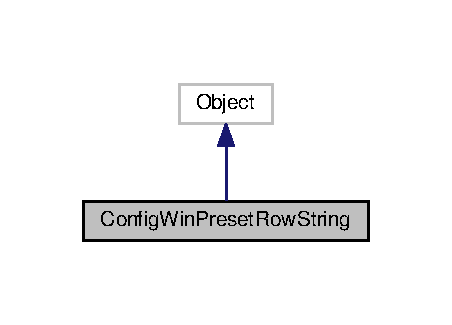
\includegraphics[width=217pt]{classConfigWinPresetRowString__inherit__graph}
\end{center}
\end{figure}


Collaboration diagram for Config\+Win\+Preset\+Row\+String\+:
\nopagebreak
\begin{figure}[H]
\begin{center}
\leavevmode
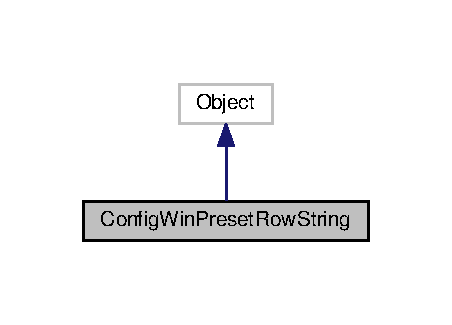
\includegraphics[width=217pt]{classConfigWinPresetRowString__coll__graph}
\end{center}
\end{figure}
\subsection*{Public Member Functions}
\begin{DoxyCompactItemize}
\item 
\mbox{\Hypertarget{classConfigWinPresetRowString_a2871b4929cbecec8e112558ff665deba}\label{classConfigWinPresetRowString_a2871b4929cbecec8e112558ff665deba}} 
\hyperlink{classConfigWinPresetRowString_a2871b4929cbecec8e112558ff665deba}{Config\+Win\+Preset\+Row\+String} (String$^\wedge$ name\+T\+MP, String$^\wedge$ preset\+T\+MP)
\begin{DoxyCompactList}\small\item\em Construct a row with a given name and command. \end{DoxyCompactList}\item 
\mbox{\Hypertarget{classConfigWinPresetRowString_a1178618ba4646cb9ee0e15f17ee72765}\label{classConfigWinPresetRowString_a1178618ba4646cb9ee0e15f17ee72765}} 
\hyperlink{classConfigWinPresetRowString_a1178618ba4646cb9ee0e15f17ee72765}{Config\+Win\+Preset\+Row\+String} (const struct \hyperlink{structPreset}{Preset} preset)
\begin{DoxyCompactList}\small\item\em Construct a row from a preset struct. \end{DoxyCompactList}\end{DoxyCompactItemize}
\subsection*{Properties}
\begin{DoxyCompactItemize}
\item 
\mbox{\Hypertarget{classConfigWinPresetRowString_a0cdef9b0f258405fac95cfcc9cf80fcb}\label{classConfigWinPresetRowString_a0cdef9b0f258405fac95cfcc9cf80fcb}} 
String$^\wedge$ \hyperlink{classConfigWinPresetRowString_a0cdef9b0f258405fac95cfcc9cf80fcb}{Name}
\begin{DoxyCompactList}\small\item\em The name given to the preset. \end{DoxyCompactList}\item 
\mbox{\Hypertarget{classConfigWinPresetRowString_a34edda87e11678d1fb024c4be4477011}\label{classConfigWinPresetRowString_a34edda87e11678d1fb024c4be4477011}} 
String$^\wedge$ \hyperlink{classConfigWinPresetRowString_a34edda87e11678d1fb024c4be4477011}{Preset}
\begin{DoxyCompactList}\small\item\em The command associated with the preset. \end{DoxyCompactList}\end{DoxyCompactItemize}


\subsection{Detailed Description}
A row in the list of presets. 

The documentation for this class was generated from the following file\+:\begin{DoxyCompactItemize}
\item 
src/Config\+Win\+Preset\+Data\+Source.\+hpp\end{DoxyCompactItemize}

\hypertarget{classConfigWinPresetTableView}{}\section{Config\+Win\+Preset\+Table\+View Class Reference}
\label{classConfigWinPresetTableView}\index{Config\+Win\+Preset\+Table\+View@{Config\+Win\+Preset\+Table\+View}}


A list of presets.  




{\ttfamily \#include $<$Config\+Win\+Preset\+Table\+View.\+hpp$>$}



Inheritance diagram for Config\+Win\+Preset\+Table\+View\+:
\nopagebreak
\begin{figure}[H]
\begin{center}
\leavevmode
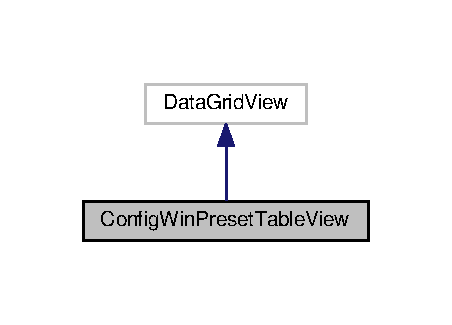
\includegraphics[width=217pt]{classConfigWinPresetTableView__inherit__graph}
\end{center}
\end{figure}


Collaboration diagram for Config\+Win\+Preset\+Table\+View\+:
\nopagebreak
\begin{figure}[H]
\begin{center}
\leavevmode
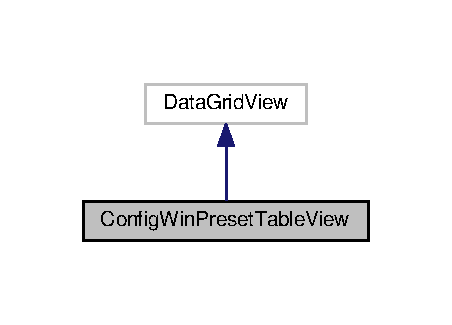
\includegraphics[width=217pt]{classConfigWinPresetTableView__coll__graph}
\end{center}
\end{figure}
\subsection*{Public Member Functions}
\begin{DoxyCompactItemize}
\item 
\mbox{\Hypertarget{classConfigWinPresetTableView_a71eeee3a1ef00851c6594cee65c511b6}\label{classConfigWinPresetTableView_a71eeee3a1ef00851c6594cee65c511b6}} 
\hyperlink{classConfigWinPresetTableView_a71eeee3a1ef00851c6594cee65c511b6}{Config\+Win\+Preset\+Table\+View} (\hyperlink{classCVDJartnet}{C\+V\+D\+Jartnet} $\ast$vdj\+Artnet)
\begin{DoxyCompactList}\small\item\em Construct a list of presets with the given instance of the plugin. \end{DoxyCompactList}\item 
\mbox{\Hypertarget{classConfigWinPresetTableView_a04e633a3caed23df0e163ee2b149868f}\label{classConfigWinPresetTableView_a04e633a3caed23df0e163ee2b149868f}} 
Data\+Object $^\wedge$ \hyperlink{classConfigWinPresetTableView_a04e633a3caed23df0e163ee2b149868f}{Get\+Clipboard\+Content} () override
\begin{DoxyCompactList}\small\item\em Get the command to be copied. \end{DoxyCompactList}\item 
\mbox{\Hypertarget{classConfigWinPresetTableView_af04fd0fbb22bbdbb9a8069f7ecf619bb}\label{classConfigWinPresetTableView_af04fd0fbb22bbdbb9a8069f7ecf619bb}} 
void \hyperlink{classConfigWinPresetTableView_af04fd0fbb22bbdbb9a8069f7ecf619bb}{table\+View\+Mouse\+Down} (Object$^\wedge$ sender, Mouse\+Event\+Args$^\wedge$ e)
\begin{DoxyCompactList}\small\item\em The mouse has been clicked. \end{DoxyCompactList}\item 
\mbox{\Hypertarget{classConfigWinPresetTableView_a68628baf1374a039651efc67ae020ac4}\label{classConfigWinPresetTableView_a68628baf1374a039651efc67ae020ac4}} 
void \hyperlink{classConfigWinPresetTableView_a68628baf1374a039651efc67ae020ac4}{table\+View\+Mouse\+Move} (Object$^\wedge$ sender, Mouse\+Event\+Args$^\wedge$ e)
\begin{DoxyCompactList}\small\item\em The mouse has been moved. \end{DoxyCompactList}\end{DoxyCompactItemize}
\subsection*{Private Attributes}
\begin{DoxyCompactItemize}
\item 
\mbox{\Hypertarget{classConfigWinPresetTableView_ad49a364287a1809859d1b6b62a40ca93}\label{classConfigWinPresetTableView_ad49a364287a1809859d1b6b62a40ca93}} 
Config\+Win\+Preset\+Data\+Source $^\wedge$ \hyperlink{classConfigWinPresetTableView_ad49a364287a1809859d1b6b62a40ca93}{data\+Source}
\begin{DoxyCompactList}\small\item\em The data source for the list. \end{DoxyCompactList}\item 
\mbox{\Hypertarget{classConfigWinPresetTableView_a773fceaf2e0a1986710eec5ea0e607a4}\label{classConfigWinPresetTableView_a773fceaf2e0a1986710eec5ea0e607a4}} 
Data\+Grid\+View\+Row $^\wedge$ \hyperlink{classConfigWinPresetTableView_a773fceaf2e0a1986710eec5ea0e607a4}{row\+To\+Drag}
\begin{DoxyCompactList}\small\item\em The row to drag. \end{DoxyCompactList}\item 
\mbox{\Hypertarget{classConfigWinPresetTableView_aaf3fd800981c4994253f0f7adb2c1581}\label{classConfigWinPresetTableView_aaf3fd800981c4994253f0f7adb2c1581}} 
System\+::\+Drawing\+::\+Rectangle \hyperlink{classConfigWinPresetTableView_aaf3fd800981c4994253f0f7adb2c1581}{drag\+Box\+From\+Mouse\+Down}
\begin{DoxyCompactList}\small\item\em A box around the initial click point. \end{DoxyCompactList}\end{DoxyCompactItemize}


\subsection{Detailed Description}
A list of presets. 

The documentation for this class was generated from the following files\+:\begin{DoxyCompactItemize}
\item 
src/Config\+Win\+Preset\+Table\+View.\+hpp\item 
src/Config\+Win\+Preset\+Table\+View.\+cpp\end{DoxyCompactItemize}

\hypertarget{classConfigWinPresetWindow}{}\section{Config\+Win\+Preset\+Window Class Reference}
\label{classConfigWinPresetWindow}\index{Config\+Win\+Preset\+Window@{Config\+Win\+Preset\+Window}}


A window containing a list of presets.  




{\ttfamily \#include $<$Config\+Win\+Preset\+Window.\+hpp$>$}



Inheritance diagram for Config\+Win\+Preset\+Window\+:
\nopagebreak
\begin{figure}[H]
\begin{center}
\leavevmode
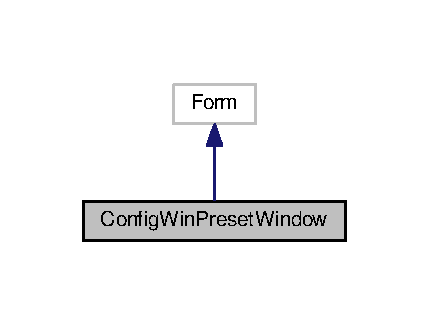
\includegraphics[width=206pt]{classConfigWinPresetWindow__inherit__graph}
\end{center}
\end{figure}


Collaboration diagram for Config\+Win\+Preset\+Window\+:
\nopagebreak
\begin{figure}[H]
\begin{center}
\leavevmode
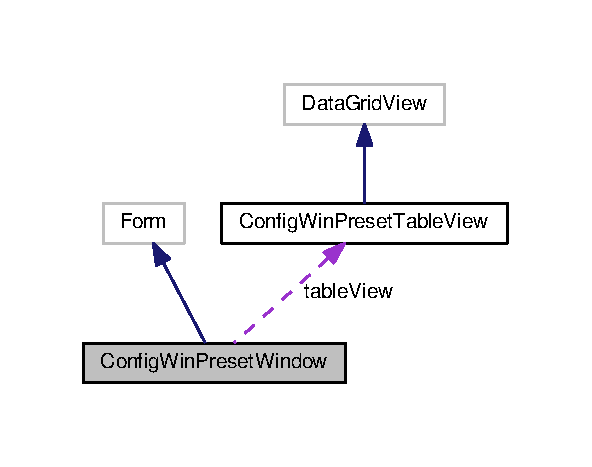
\includegraphics[width=284pt]{classConfigWinPresetWindow__coll__graph}
\end{center}
\end{figure}
\subsection*{Public Member Functions}
\begin{DoxyCompactItemize}
\item 
\mbox{\Hypertarget{classConfigWinPresetWindow_aaa53b5d271475994781c405cddb81d90}\label{classConfigWinPresetWindow_aaa53b5d271475994781c405cddb81d90}} 
\hyperlink{classConfigWinPresetWindow_aaa53b5d271475994781c405cddb81d90}{Config\+Win\+Preset\+Window} (\hyperlink{classCVDJartnet}{C\+V\+D\+Jartnet} $\ast$vdj\+Artnet\+T\+MP)
\begin{DoxyCompactList}\small\item\em Construct a window with a list of presets with the given instance of the plugin. \end{DoxyCompactList}\item 
\mbox{\Hypertarget{classConfigWinPresetWindow_ae821eddfb5203330ef3731a0a4367b48}\label{classConfigWinPresetWindow_ae821eddfb5203330ef3731a0a4367b48}} 
void \hyperlink{classConfigWinPresetWindow_ae821eddfb5203330ef3731a0a4367b48}{re\+Layout} (Object$^\wedge$ sender, Layout\+Event\+Args$^\wedge$ e)
\begin{DoxyCompactList}\small\item\em Relayout the window. \end{DoxyCompactList}\end{DoxyCompactItemize}
\subsection*{Private Attributes}
\begin{DoxyCompactItemize}
\item 
\mbox{\Hypertarget{classConfigWinPresetWindow_a39234b6105a76a2864775e51d53ea719}\label{classConfigWinPresetWindow_a39234b6105a76a2864775e51d53ea719}} 
\hyperlink{classConfigWinPresetTableView}{Config\+Win\+Preset\+Table\+View} $^\wedge$ \hyperlink{classConfigWinPresetWindow_a39234b6105a76a2864775e51d53ea719}{table\+View}
\begin{DoxyCompactList}\small\item\em The list of preset. \end{DoxyCompactList}\end{DoxyCompactItemize}


\subsection{Detailed Description}
A window containing a list of presets. 

The documentation for this class was generated from the following files\+:\begin{DoxyCompactItemize}
\item 
src/Config\+Win\+Preset\+Window.\+hpp\item 
src/Config\+Win\+Preset\+Window.\+cpp\end{DoxyCompactItemize}

\hypertarget{classConfigWinRowString}{}\section{Config\+Win\+Row\+String Class Reference}
\label{classConfigWinRowString}\index{Config\+Win\+Row\+String@{Config\+Win\+Row\+String}}


A row in the list of commands in the config tool.  




{\ttfamily \#include $<$Config\+Win\+Data\+Source.\+hpp$>$}



Inheritance diagram for Config\+Win\+Row\+String\+:
\nopagebreak
\begin{figure}[H]
\begin{center}
\leavevmode
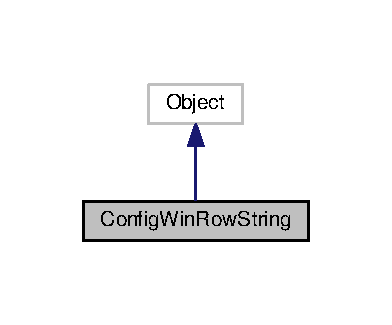
\includegraphics[width=188pt]{classConfigWinRowString__inherit__graph}
\end{center}
\end{figure}


Collaboration diagram for Config\+Win\+Row\+String\+:
\nopagebreak
\begin{figure}[H]
\begin{center}
\leavevmode
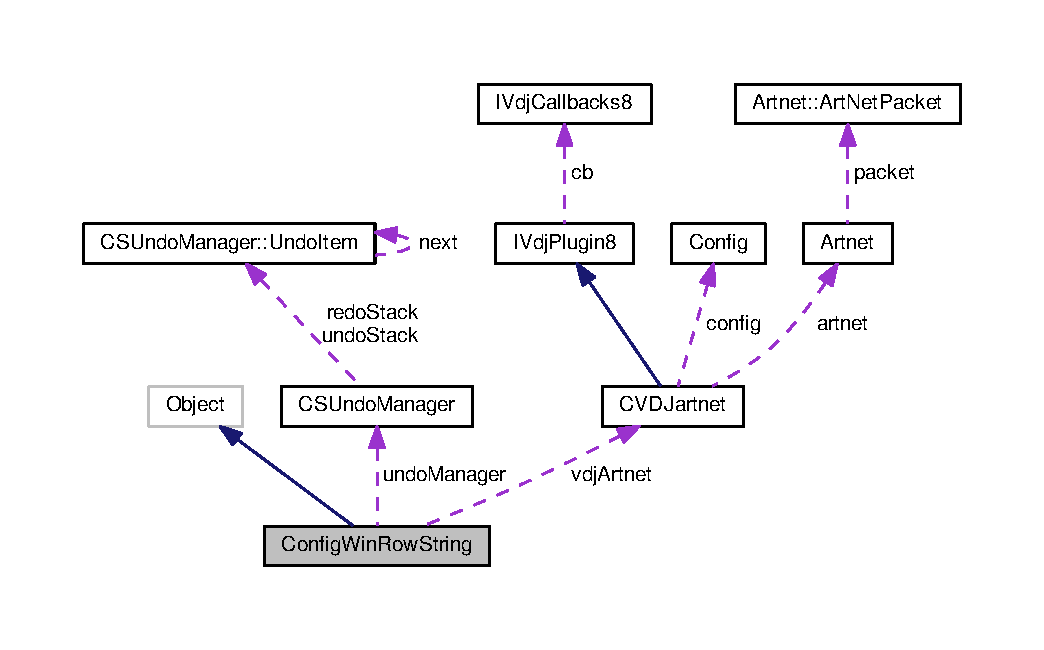
\includegraphics[width=350pt]{classConfigWinRowString__coll__graph}
\end{center}
\end{figure}
\subsection*{Public Member Functions}
\begin{DoxyCompactItemize}
\item 
\mbox{\Hypertarget{classConfigWinRowString_a1c009e54fd745979399fcbf33949341b}\label{classConfigWinRowString_a1c009e54fd745979399fcbf33949341b}} 
\hyperlink{classConfigWinRowString_a1c009e54fd745979399fcbf33949341b}{Config\+Win\+Row\+String} (\hyperlink{classCVDJartnet}{C\+V\+D\+Jartnet} $\ast$vdj\+Artnet\+T\+MP, int row\+T\+MP, \hyperlink{classCSUndoManager}{C\+S\+Undo\+Manager} $\ast$undo\+Manager\+T\+MP)
\begin{DoxyCompactList}\small\item\em Construct a row with the given instance of the plugin, row number and undo manager. \end{DoxyCompactList}\end{DoxyCompactItemize}
\subsection*{Properties}
\begin{DoxyCompactItemize}
\item 
String$^\wedge$ \hyperlink{classConfigWinRowString_ad8324c1c0df6f0069626c15119539e6c}{Value}\hspace{0.3cm}{\ttfamily  \mbox{[}get, set\mbox{]}}
\begin{DoxyCompactList}\small\item\em The value of the command. \end{DoxyCompactList}\end{DoxyCompactItemize}
\subsection*{Private Attributes}
\begin{DoxyCompactItemize}
\item 
\mbox{\Hypertarget{classConfigWinRowString_a71a5621146c28fcbc9418079a15d367e}\label{classConfigWinRowString_a71a5621146c28fcbc9418079a15d367e}} 
\hyperlink{classCVDJartnet}{C\+V\+D\+Jartnet} $\ast$ \hyperlink{classConfigWinRowString_a71a5621146c28fcbc9418079a15d367e}{vdj\+Artnet}
\begin{DoxyCompactList}\small\item\em A pointer to the plugin. \end{DoxyCompactList}\item 
\mbox{\Hypertarget{classConfigWinRowString_a6b3d9b4d2c7775ea440a52ef78697d87}\label{classConfigWinRowString_a6b3d9b4d2c7775ea440a52ef78697d87}} 
int \hyperlink{classConfigWinRowString_a6b3d9b4d2c7775ea440a52ef78697d87}{row}
\begin{DoxyCompactList}\small\item\em The number of this row. \end{DoxyCompactList}\item 
\mbox{\Hypertarget{classConfigWinRowString_a3941099a204c34f3f76a9a582c8cfb8c}\label{classConfigWinRowString_a3941099a204c34f3f76a9a582c8cfb8c}} 
\hyperlink{classCSUndoManager}{C\+S\+Undo\+Manager} $\ast$ \hyperlink{classConfigWinRowString_a3941099a204c34f3f76a9a582c8cfb8c}{undo\+Manager}
\begin{DoxyCompactList}\small\item\em A pointer to the undo manager. \end{DoxyCompactList}\end{DoxyCompactItemize}


\subsection{Detailed Description}
A row in the list of commands in the config tool. 

\subsection{Property Documentation}
\mbox{\Hypertarget{classConfigWinRowString_ad8324c1c0df6f0069626c15119539e6c}\label{classConfigWinRowString_ad8324c1c0df6f0069626c15119539e6c}} 
\index{Config\+Win\+Row\+String@{Config\+Win\+Row\+String}!Value@{Value}}
\index{Value@{Value}!Config\+Win\+Row\+String@{Config\+Win\+Row\+String}}
\subsubsection{\texorpdfstring{Value}{Value}}
{\footnotesize\ttfamily String$^\wedge$ Config\+Win\+Row\+String\+::\+Value\hspace{0.3cm}{\ttfamily [get]}, {\ttfamily [set]}}



The value of the command. 



The documentation for this class was generated from the following files\+:\begin{DoxyCompactItemize}
\item 
src/\hyperlink{ConfigWinDataSource_8hpp}{Config\+Win\+Data\+Source.\+hpp}\item 
src/Config\+Win\+Data\+Source.\+cpp\end{DoxyCompactItemize}

\hypertarget{classConfigWinTableView}{}\section{Config\+Win\+Table\+View Class Reference}
\label{classConfigWinTableView}\index{Config\+Win\+Table\+View@{Config\+Win\+Table\+View}}


A list of commands.  




{\ttfamily \#include $<$Config\+Win\+Table\+View.\+hpp$>$}



Inheritance diagram for Config\+Win\+Table\+View\+:
\nopagebreak
\begin{figure}[H]
\begin{center}
\leavevmode
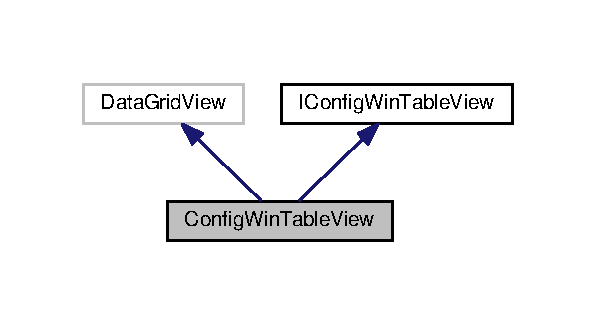
\includegraphics[width=286pt]{classConfigWinTableView__inherit__graph}
\end{center}
\end{figure}


Collaboration diagram for Config\+Win\+Table\+View\+:
\nopagebreak
\begin{figure}[H]
\begin{center}
\leavevmode
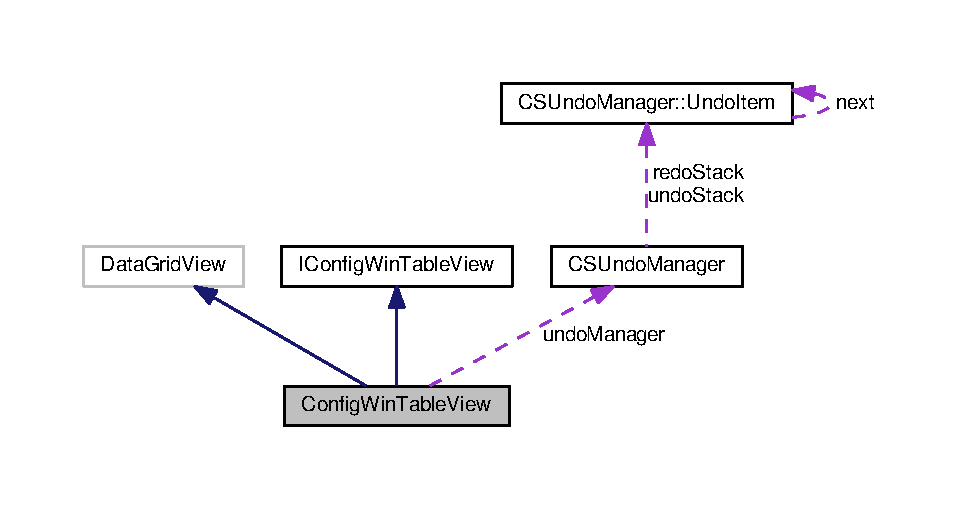
\includegraphics[width=350pt]{classConfigWinTableView__coll__graph}
\end{center}
\end{figure}
\subsection*{Public Member Functions}
\begin{DoxyCompactItemize}
\item 
\mbox{\Hypertarget{classConfigWinTableView_a12104b4ce88342f5c6e75d3aafc57535}\label{classConfigWinTableView_a12104b4ce88342f5c6e75d3aafc57535}} 
virtual bool \hyperlink{classConfigWinTableView_a12104b4ce88342f5c6e75d3aafc57535}{Process\+Cmd\+Key} (Message\% msg, Keys key\+Data) override
\begin{DoxyCompactList}\small\item\em A process a key press. \end{DoxyCompactList}\item 
\mbox{\Hypertarget{classConfigWinTableView_a7b0abcafca070a2581de9d13fbcf7477}\label{classConfigWinTableView_a7b0abcafca070a2581de9d13fbcf7477}} 
\hyperlink{classConfigWinTableView_a7b0abcafca070a2581de9d13fbcf7477}{Config\+Win\+Table\+View} (\hyperlink{classCVDJartnet}{C\+V\+D\+Jartnet} $\ast$vdj\+Artnet)
\begin{DoxyCompactList}\small\item\em Construct a list of commands with the given instance of the plugin. \end{DoxyCompactList}\item 
\mbox{\Hypertarget{classConfigWinTableView_a99ca2c9d181ad0370c156fb648ed3a0e}\label{classConfigWinTableView_a99ca2c9d181ad0370c156fb648ed3a0e}} 
void \hyperlink{classConfigWinTableView_a99ca2c9d181ad0370c156fb648ed3a0e}{table\+View\+Key\+Down} (Object$^\wedge$ sender, Key\+Event\+Args$^\wedge$ e)
\begin{DoxyCompactList}\small\item\em A key has been pressed. \end{DoxyCompactList}\item 
\mbox{\Hypertarget{classConfigWinTableView_ad78543f2ff3cb851b0f591c9f0219b0c}\label{classConfigWinTableView_ad78543f2ff3cb851b0f591c9f0219b0c}} 
void \hyperlink{classConfigWinTableView_ad78543f2ff3cb851b0f591c9f0219b0c}{table\+View\+Editing\+Control\+Showing} (Object$^\wedge$ sender, Data\+Grid\+View\+Editing\+Control\+Showing\+Event\+Args$^\wedge$ e)
\begin{DoxyCompactList}\small\item\em A cell is about to be shown. \end{DoxyCompactList}\item 
\mbox{\Hypertarget{classConfigWinTableView_a442481e0961b30b66795fb3e03b652e2}\label{classConfigWinTableView_a442481e0961b30b66795fb3e03b652e2}} 
void \hyperlink{classConfigWinTableView_a442481e0961b30b66795fb3e03b652e2}{table\+View\+Mouse\+Down} (Object$^\wedge$ sender, Mouse\+Event\+Args$^\wedge$ e)
\begin{DoxyCompactList}\small\item\em The mouse has been clicked. \end{DoxyCompactList}\item 
\mbox{\Hypertarget{classConfigWinTableView_a24eb847e5dbac7375fba96a718dea5fc}\label{classConfigWinTableView_a24eb847e5dbac7375fba96a718dea5fc}} 
void \hyperlink{classConfigWinTableView_a24eb847e5dbac7375fba96a718dea5fc}{table\+View\+Mouse\+Move} (Object$^\wedge$ sender, Mouse\+Event\+Args$^\wedge$ e)
\begin{DoxyCompactList}\small\item\em The mouse has been moved. \end{DoxyCompactList}\item 
\mbox{\Hypertarget{classConfigWinTableView_a43523fa68d77c79b1bb62430db018dd1}\label{classConfigWinTableView_a43523fa68d77c79b1bb62430db018dd1}} 
void \hyperlink{classConfigWinTableView_a43523fa68d77c79b1bb62430db018dd1}{table\+View\+Drag\+Enter} (Object$^\wedge$ sender, Drag\+Event\+Args$^\wedge$ e)
\begin{DoxyCompactList}\small\item\em A dragged object has entered the list. \end{DoxyCompactList}\item 
\mbox{\Hypertarget{classConfigWinTableView_a8a74aaf5e91957b5669f94c7e7741f61}\label{classConfigWinTableView_a8a74aaf5e91957b5669f94c7e7741f61}} 
void \hyperlink{classConfigWinTableView_a8a74aaf5e91957b5669f94c7e7741f61}{table\+View\+Drag\+Drop} (Object$^\wedge$ sender, Drag\+Event\+Args$^\wedge$ e)
\begin{DoxyCompactList}\small\item\em A dragged object has been dropped in the list. \end{DoxyCompactList}\end{DoxyCompactItemize}
\subsection*{Events}
\begin{DoxyCompactItemize}
\item 
\mbox{\Hypertarget{classConfigWinTableView_a1d83b0981b052d268c7ddc6e9b4a897b}\label{classConfigWinTableView_a1d83b0981b052d268c7ddc6e9b4a897b}} 
virtual Config\+Win\+Table\+View\+Key\+Event\+Handler$^\wedge$ \hyperlink{classConfigWinTableView_a1d83b0981b052d268c7ddc6e9b4a897b}{Config\+Table\+View\+Key\+Down}
\begin{DoxyCompactList}\small\item\em A key has been pressed. \end{DoxyCompactList}\end{DoxyCompactItemize}
\subsection*{Private Attributes}
\begin{DoxyCompactItemize}
\item 
\mbox{\Hypertarget{classConfigWinTableView_a17e877f059f696a751ee9e765c699b16}\label{classConfigWinTableView_a17e877f059f696a751ee9e765c699b16}} 
Data\+Grid\+View\+Row $^\wedge$ \hyperlink{classConfigWinTableView_a17e877f059f696a751ee9e765c699b16}{row\+To\+Drag}
\begin{DoxyCompactList}\small\item\em The row to drag. \end{DoxyCompactList}\item 
\mbox{\Hypertarget{classConfigWinTableView_a4e0a1429fe25686c0d458dd444593ced}\label{classConfigWinTableView_a4e0a1429fe25686c0d458dd444593ced}} 
System\+::\+Drawing\+::\+Rectangle \hyperlink{classConfigWinTableView_a4e0a1429fe25686c0d458dd444593ced}{drag\+Box\+From\+Mouse\+Down}
\begin{DoxyCompactList}\small\item\em A box around the initial click point. \end{DoxyCompactList}\item 
\mbox{\Hypertarget{classConfigWinTableView_ac99d78aaac737402e3ef047597bb77fa}\label{classConfigWinTableView_ac99d78aaac737402e3ef047597bb77fa}} 
\hyperlink{classCSUndoManager}{C\+S\+Undo\+Manager} $\ast$ \hyperlink{classConfigWinTableView_ac99d78aaac737402e3ef047597bb77fa}{undo\+Manager}
\begin{DoxyCompactList}\small\item\em A pointer to the undo manager. \end{DoxyCompactList}\end{DoxyCompactItemize}


\subsection{Detailed Description}
A list of commands. 

The documentation for this class was generated from the following files\+:\begin{DoxyCompactItemize}
\item 
src/Config\+Win\+Table\+View.\+hpp\item 
src/Config\+Win\+Table\+View.\+cpp\end{DoxyCompactItemize}

\hypertarget{classConfigWinTool}{}\section{Config\+Win\+Tool Class Reference}
\label{classConfigWinTool}\index{Config\+Win\+Tool@{Config\+Win\+Tool}}


A config tool to help the user write a correctly formatted config file.  




{\ttfamily \#include $<$Config\+Win.\+hpp$>$}



Collaboration diagram for Config\+Win\+Tool\+:
\nopagebreak
\begin{figure}[H]
\begin{center}
\leavevmode
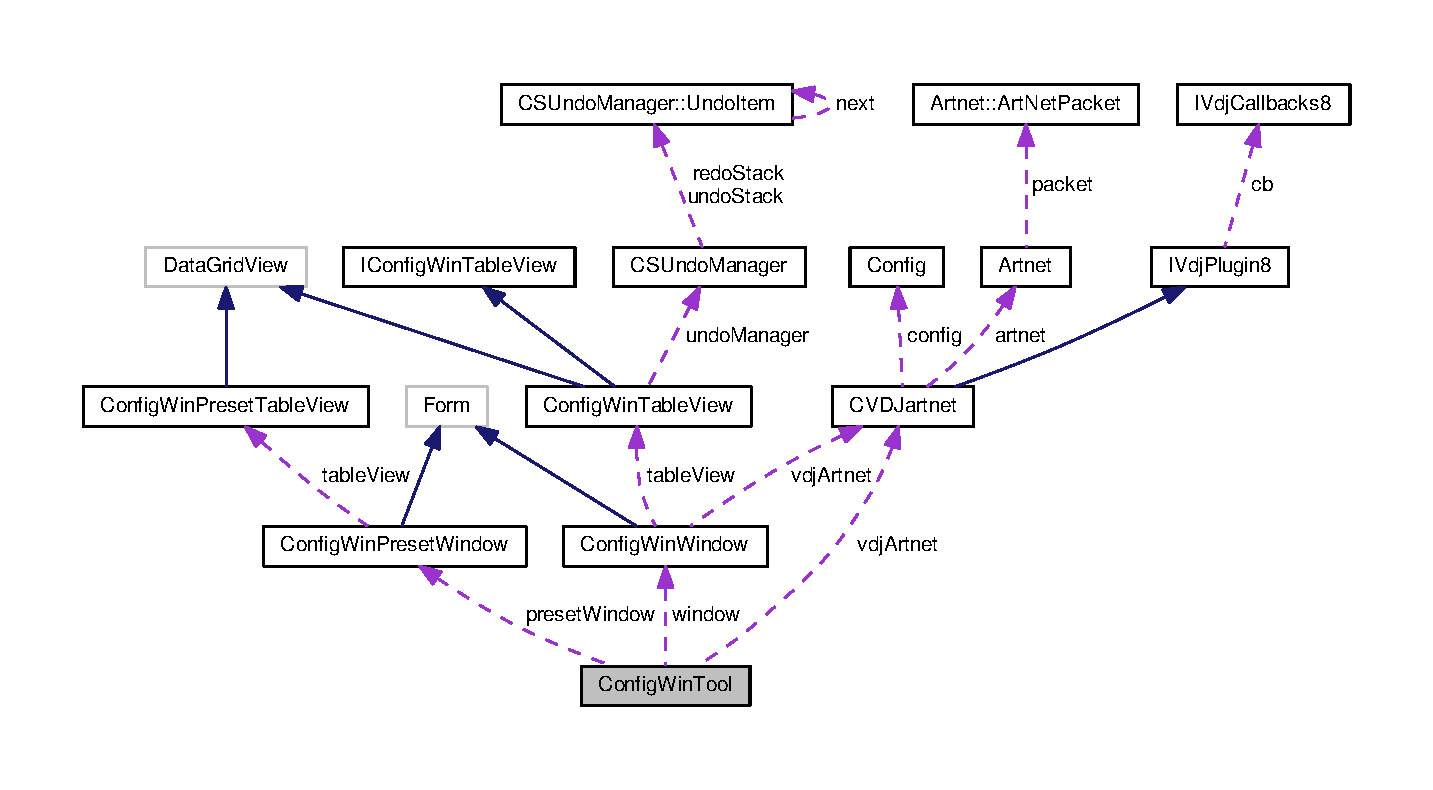
\includegraphics[width=350pt]{classConfigWinTool__coll__graph}
\end{center}
\end{figure}
\subsection*{Public Member Functions}
\begin{DoxyCompactItemize}
\item 
\mbox{\Hypertarget{classConfigWinTool_a4aea1c2bd45e724b3034446f5e71cd14}\label{classConfigWinTool_a4aea1c2bd45e724b3034446f5e71cd14}} 
\hyperlink{classConfigWinTool_a4aea1c2bd45e724b3034446f5e71cd14}{Config\+Win\+Tool} (\hyperlink{classCVDJartnet}{C\+V\+D\+Jartnet} $\ast$vdj\+Artnet\+T\+MP)
\begin{DoxyCompactList}\small\item\em Construct a config tool with the given instance of the plugin. \end{DoxyCompactList}\item 
\mbox{\Hypertarget{classConfigWinTool_affa13cd91024a6d11997fa2577bf473e}\label{classConfigWinTool_affa13cd91024a6d11997fa2577bf473e}} 
void \hyperlink{classConfigWinTool_affa13cd91024a6d11997fa2577bf473e}{hide} ()
\begin{DoxyCompactList}\small\item\em Hide the config tool after the user has finished. \end{DoxyCompactList}\end{DoxyCompactItemize}
\subsection*{Private Attributes}
\begin{DoxyCompactItemize}
\item 
\mbox{\Hypertarget{classConfigWinTool_a3dc8349b61bb9da1c299a56a1397b7bf}\label{classConfigWinTool_a3dc8349b61bb9da1c299a56a1397b7bf}} 
\hyperlink{classCVDJartnet}{C\+V\+D\+Jartnet} $\ast$ \hyperlink{classConfigWinTool_a3dc8349b61bb9da1c299a56a1397b7bf}{vdj\+Artnet}
\begin{DoxyCompactList}\small\item\em A pointer to the plugin. \end{DoxyCompactList}\item 
\mbox{\Hypertarget{classConfigWinTool_af36be9ee4967921063c85c2e715610d9}\label{classConfigWinTool_af36be9ee4967921063c85c2e715610d9}} 
\hyperlink{classConfigWinWindow}{Config\+Win\+Window} $^\wedge$ \hyperlink{classConfigWinTool_af36be9ee4967921063c85c2e715610d9}{window}
\begin{DoxyCompactList}\small\item\em The main window representing the config file. \end{DoxyCompactList}\item 
\mbox{\Hypertarget{classConfigWinTool_a95d26aef64982f0ed56b9db4d3694d6f}\label{classConfigWinTool_a95d26aef64982f0ed56b9db4d3694d6f}} 
\hyperlink{classConfigWinPresetWindow}{Config\+Win\+Preset\+Window} $^\wedge$ \hyperlink{classConfigWinTool_a95d26aef64982f0ed56b9db4d3694d6f}{preset\+Window}
\begin{DoxyCompactList}\small\item\em A window with presets representing common config lines. \end{DoxyCompactList}\end{DoxyCompactItemize}


\subsection{Detailed Description}
A config tool to help the user write a correctly formatted config file. 

The documentation for this class was generated from the following files\+:\begin{DoxyCompactItemize}
\item 
src/\hyperlink{ConfigWin_8hpp}{Config\+Win.\+hpp}\item 
src/Config\+Win.\+cpp\end{DoxyCompactItemize}

\hypertarget{classConfigWinToolNative}{}\section{Config\+Win\+Tool\+Native Class Reference}
\label{classConfigWinToolNative}\index{Config\+Win\+Tool\+Native@{Config\+Win\+Tool\+Native}}


An unmanaged wrapper around \hyperlink{classConfigWinTool}{Config\+Win\+Tool}.  




{\ttfamily \#include $<$Config\+Win.\+hpp$>$}

\subsection*{Public Member Functions}
\begin{DoxyCompactItemize}
\item 
\mbox{\Hypertarget{classConfigWinToolNative_a7042b5af4bdfe4dc1b8fbfb156c4b188}\label{classConfigWinToolNative_a7042b5af4bdfe4dc1b8fbfb156c4b188}} 
\hyperlink{classConfigWinToolNative_a7042b5af4bdfe4dc1b8fbfb156c4b188}{Config\+Win\+Tool\+Native} (\hyperlink{classCVDJartnet}{C\+V\+D\+Jartnet} $\ast$vdj\+Artnet)
\begin{DoxyCompactList}\small\item\em Construct the managed \hyperlink{classConfigWinTool}{Config\+Win\+Tool}. \end{DoxyCompactList}\end{DoxyCompactItemize}
\subsection*{Public Attributes}
\begin{DoxyCompactItemize}
\item 
\mbox{\Hypertarget{classConfigWinToolNative_a8bdff36b89c6091b360b75866c4da346}\label{classConfigWinToolNative_a8bdff36b89c6091b360b75866c4da346}} 
msclr\+::gcroot$<$ \hyperlink{classConfigWinTool}{Config\+Win\+Tool}$^\wedge$$>$ \hyperlink{classConfigWinToolNative_a8bdff36b89c6091b360b75866c4da346}{config\+Tool}
\begin{DoxyCompactList}\small\item\em The managed \hyperlink{classConfigWinTool}{Config\+Win\+Tool}. \end{DoxyCompactList}\end{DoxyCompactItemize}


\subsection{Detailed Description}
An unmanaged wrapper around \hyperlink{classConfigWinTool}{Config\+Win\+Tool}. 

This is needed so that it can be instanciated from code that isn\textquotesingle{}t compiled with the C\+LR. 

The documentation for this class was generated from the following file\+:\begin{DoxyCompactItemize}
\item 
src/\hyperlink{ConfigWin_8hpp}{Config\+Win.\+hpp}\end{DoxyCompactItemize}

\hypertarget{classConfigWinWindow}{}\section{Config\+Win\+Window Class Reference}
\label{classConfigWinWindow}\index{Config\+Win\+Window@{Config\+Win\+Window}}


A window containing a list of commands.  




{\ttfamily \#include $<$Config\+Win\+Window.\+hpp$>$}



Inheritance diagram for Config\+Win\+Window\+:
\nopagebreak
\begin{figure}[H]
\begin{center}
\leavevmode
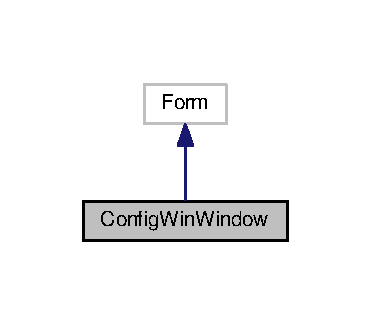
\includegraphics[width=178pt]{classConfigWinWindow__inherit__graph}
\end{center}
\end{figure}


Collaboration diagram for Config\+Win\+Window\+:
\nopagebreak
\begin{figure}[H]
\begin{center}
\leavevmode
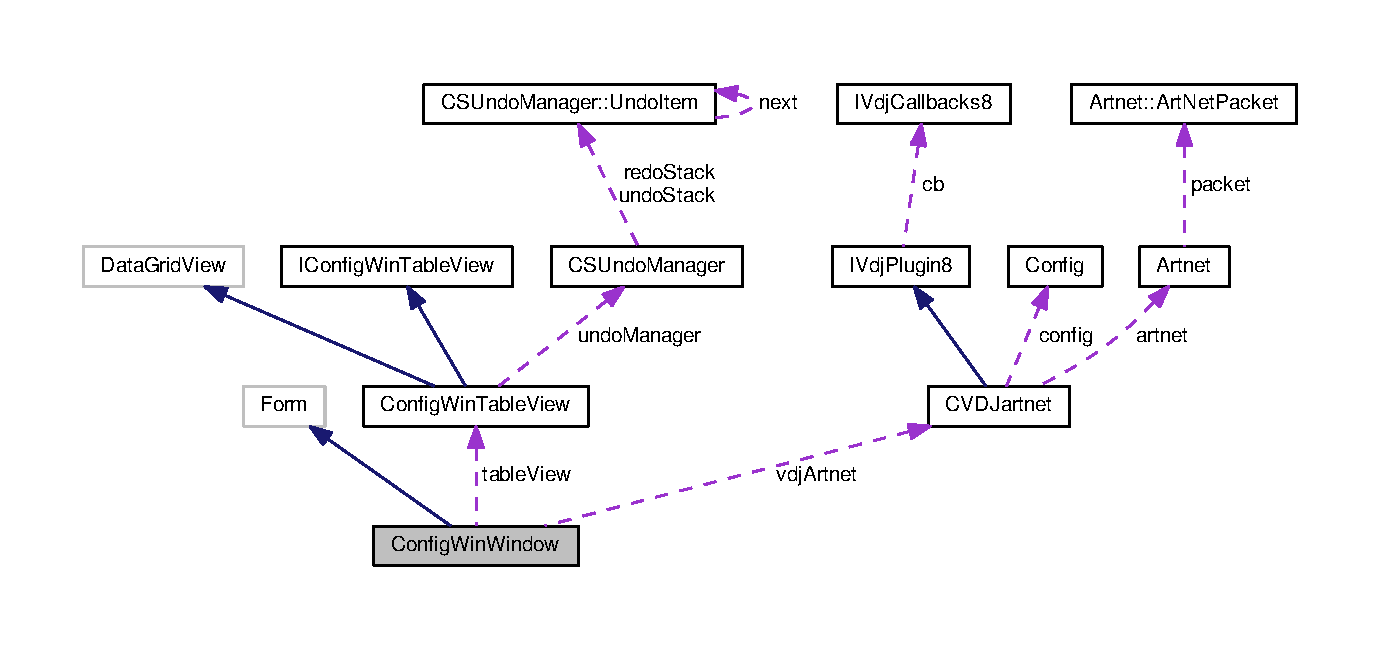
\includegraphics[width=350pt]{classConfigWinWindow__coll__graph}
\end{center}
\end{figure}
\subsection*{Public Member Functions}
\begin{DoxyCompactItemize}
\item 
\mbox{\Hypertarget{classConfigWinWindow_a450c1273eeacf866a5cbdc77899c59f1}\label{classConfigWinWindow_a450c1273eeacf866a5cbdc77899c59f1}} 
\hyperlink{classConfigWinWindow_a450c1273eeacf866a5cbdc77899c59f1}{Config\+Win\+Window} (\hyperlink{classCVDJartnet}{C\+V\+D\+Jartnet} $\ast$vdj\+Artnet\+T\+MP)
\begin{DoxyCompactList}\small\item\em Construct a window with a list of commands with the given instance of the plugin. \end{DoxyCompactList}\item 
\mbox{\Hypertarget{classConfigWinWindow_a3181fb8df8491c448b0afe6011d9b71d}\label{classConfigWinWindow_a3181fb8df8491c448b0afe6011d9b71d}} 
void \hyperlink{classConfigWinWindow_a3181fb8df8491c448b0afe6011d9b71d}{re\+Layout} (Object$^\wedge$ sender, Layout\+Event\+Args$^\wedge$ e)
\begin{DoxyCompactList}\small\item\em Relayout the window. \end{DoxyCompactList}\item 
\mbox{\Hypertarget{classConfigWinWindow_af0ef395b86d59a38d4d5bb8f978c63f4}\label{classConfigWinWindow_af0ef395b86d59a38d4d5bb8f978c63f4}} 
void \hyperlink{classConfigWinWindow_af0ef395b86d59a38d4d5bb8f978c63f4}{did\+Close} (Object$^\wedge$ sender, Form\+Closed\+Event\+Args$^\wedge$ e)
\begin{DoxyCompactList}\small\item\em The window has been closed. \end{DoxyCompactList}\item 
\mbox{\Hypertarget{classConfigWinWindow_a89a9b6154e716142854ecbec1eaccb15}\label{classConfigWinWindow_a89a9b6154e716142854ecbec1eaccb15}} 
void \hyperlink{classConfigWinWindow_a89a9b6154e716142854ecbec1eaccb15}{update\+I\+Paddress} (Object$^\wedge$ sender, Event\+Args$^\wedge$ e)
\begin{DoxyCompactList}\small\item\em Update the IP address in the config. \end{DoxyCompactList}\item 
\mbox{\Hypertarget{classConfigWinWindow_ac1a7295061c09db580be48222baef958}\label{classConfigWinWindow_ac1a7295061c09db580be48222baef958}} 
void \hyperlink{classConfigWinWindow_ac1a7295061c09db580be48222baef958}{update\+I\+Pport} (Object$^\wedge$ sender, Event\+Args$^\wedge$ e)
\begin{DoxyCompactList}\small\item\em Update the port in the config. \end{DoxyCompactList}\item 
\mbox{\Hypertarget{classConfigWinWindow_a04f73656ff5be88aa0497d75557c2229}\label{classConfigWinWindow_a04f73656ff5be88aa0497d75557c2229}} 
void \hyperlink{classConfigWinWindow_a04f73656ff5be88aa0497d75557c2229}{ip\+Key\+Down} (Object$^\wedge$ sender, Key\+Event\+Args$^\wedge$ e)
\begin{DoxyCompactList}\small\item\em A key has been pressed in the IP address field. \end{DoxyCompactList}\end{DoxyCompactItemize}
\subsection*{Private Attributes}
\begin{DoxyCompactItemize}
\item 
\mbox{\Hypertarget{classConfigWinWindow_add13d144a5a011195cedd76ed259ecff}\label{classConfigWinWindow_add13d144a5a011195cedd76ed259ecff}} 
\hyperlink{classCVDJartnet}{C\+V\+D\+Jartnet} $\ast$ \hyperlink{classConfigWinWindow_add13d144a5a011195cedd76ed259ecff}{vdj\+Artnet}
\begin{DoxyCompactList}\small\item\em A pointer to the plugin. \end{DoxyCompactList}\item 
\mbox{\Hypertarget{classConfigWinWindow_aaa2e34f0cf75b85f6da371baa86e4eac}\label{classConfigWinWindow_aaa2e34f0cf75b85f6da371baa86e4eac}} 
Label $^\wedge$ \hyperlink{classConfigWinWindow_aaa2e34f0cf75b85f6da371baa86e4eac}{ip\+Label}
\begin{DoxyCompactList}\small\item\em A label for the IP address field. \end{DoxyCompactList}\item 
\mbox{\Hypertarget{classConfigWinWindow_af41aee8bafd96f1e86fbc900dccadc45}\label{classConfigWinWindow_af41aee8bafd96f1e86fbc900dccadc45}} 
Text\+Box $^\wedge$ \hyperlink{classConfigWinWindow_af41aee8bafd96f1e86fbc900dccadc45}{ip\+Address}
\begin{DoxyCompactList}\small\item\em The IP address field. \end{DoxyCompactList}\item 
\mbox{\Hypertarget{classConfigWinWindow_a383e4fe684dbe4e040cfcee7ec2034d9}\label{classConfigWinWindow_a383e4fe684dbe4e040cfcee7ec2034d9}} 
Text\+Box $^\wedge$ \hyperlink{classConfigWinWindow_a383e4fe684dbe4e040cfcee7ec2034d9}{ip\+Port}
\begin{DoxyCompactList}\small\item\em The port field. \end{DoxyCompactList}\item 
\mbox{\Hypertarget{classConfigWinWindow_a16003ab2a1160a652d4cc1a17075d7e4}\label{classConfigWinWindow_a16003ab2a1160a652d4cc1a17075d7e4}} 
\hyperlink{classConfigWinTableView}{Config\+Win\+Table\+View} $^\wedge$ \hyperlink{classConfigWinWindow_a16003ab2a1160a652d4cc1a17075d7e4}{table\+View}
\begin{DoxyCompactList}\small\item\em The list of commands. \end{DoxyCompactList}\end{DoxyCompactItemize}


\subsection{Detailed Description}
A window containing a list of commands. 

The documentation for this class was generated from the following files\+:\begin{DoxyCompactItemize}
\item 
src/Config\+Win\+Window.\+hpp\item 
src/Config\+Win\+Window.\+cpp\end{DoxyCompactItemize}

\hypertarget{classCSUndoManager}{}\section{C\+S\+Undo\+Manager Class Reference}
\label{classCSUndoManager}\index{C\+S\+Undo\+Manager@{C\+S\+Undo\+Manager}}


An undo manager.  




{\ttfamily \#include $<$C\+S\+Undo\+Manager.\+hpp$>$}



Collaboration diagram for C\+S\+Undo\+Manager\+:
\nopagebreak
\begin{figure}[H]
\begin{center}
\leavevmode
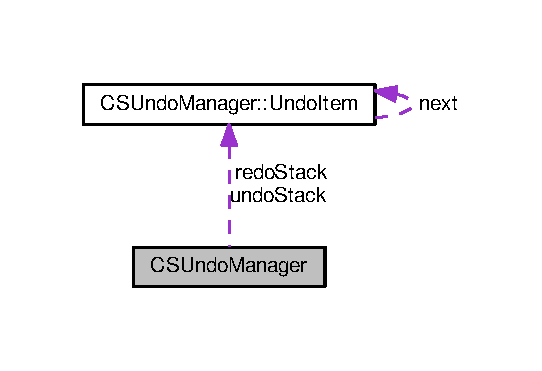
\includegraphics[width=260pt]{classCSUndoManager__coll__graph}
\end{center}
\end{figure}
\subsection*{Classes}
\begin{DoxyCompactItemize}
\item 
class \hyperlink{classCSUndoManager_1_1UndoItem}{Undo\+Item}
\begin{DoxyCompactList}\small\item\em An event that can be undone. \end{DoxyCompactList}\end{DoxyCompactItemize}
\subsection*{Public Member Functions}
\begin{DoxyCompactItemize}
\item 
\mbox{\Hypertarget{classCSUndoManager_a8195893d40647952225158b9bc883ac8}\label{classCSUndoManager_a8195893d40647952225158b9bc883ac8}} 
\hyperlink{classCSUndoManager_a8195893d40647952225158b9bc883ac8}{C\+S\+Undo\+Manager} ()
\begin{DoxyCompactList}\small\item\em Construct an undo manager. \end{DoxyCompactList}\item 
void \hyperlink{classCSUndoManager_af8b0d7f2acb9d6686cd030e1cef1640e}{register\+Undo\+Func} (std\+::function$<$ void()$>$ f)
\begin{DoxyCompactList}\small\item\em Register an undo to the stack with the given function object. \end{DoxyCompactList}\item 
\mbox{\Hypertarget{classCSUndoManager_a35d72c80c1aefbd08592a866ea18f0da}\label{classCSUndoManager_a35d72c80c1aefbd08592a866ea18f0da}} 
{\footnotesize template$<$typename T $>$ }\\void \hyperlink{classCSUndoManager_a35d72c80c1aefbd08592a866ea18f0da}{register\+Undo\+Func\+Arg} (std\+::function$<$ void(T)$>$ f, T arg)
\begin{DoxyCompactList}\small\item\em Register an undo to the stack with the given function and pair of arguments to pass it. \end{DoxyCompactList}\item 
\mbox{\Hypertarget{classCSUndoManager_af5412c615c1bb86d6e6657bab1e2175e}\label{classCSUndoManager_af5412c615c1bb86d6e6657bab1e2175e}} 
{\footnotesize template$<$typename S , typename T $>$ }\\void \hyperlink{classCSUndoManager_af5412c615c1bb86d6e6657bab1e2175e}{register\+Undo\+Funcp\+Arg2} (void($\ast$f)(S, T), S arg1, T arg2)
\begin{DoxyCompactList}\small\item\em Register an undo to the stack that restores the value of the given target. \end{DoxyCompactList}\item 
\mbox{\Hypertarget{classCSUndoManager_a7bb75a1243d60c291e6c1a6cc5d5f6a7}\label{classCSUndoManager_a7bb75a1243d60c291e6c1a6cc5d5f6a7}} 
{\footnotesize template$<$typename T $>$ }\\void {\bfseries register\+Undo\+Target} (T $\ast$target)
\item 
\mbox{\Hypertarget{classCSUndoManager_aba7234583f74080689d126d142cee5fa}\label{classCSUndoManager_aba7234583f74080689d126d142cee5fa}} 
bool \hyperlink{classCSUndoManager_aba7234583f74080689d126d142cee5fa}{can\+Undo} ()
\begin{DoxyCompactList}\small\item\em There is an undo on the stack. \end{DoxyCompactList}\item 
\mbox{\Hypertarget{classCSUndoManager_af604822084540cbee8a7b99dd6139600}\label{classCSUndoManager_af604822084540cbee8a7b99dd6139600}} 
void \hyperlink{classCSUndoManager_af604822084540cbee8a7b99dd6139600}{undo} ()
\begin{DoxyCompactList}\small\item\em Undo the last value from the undo stack. \end{DoxyCompactList}\item 
\mbox{\Hypertarget{classCSUndoManager_aac205c66f6620adc3785321f52679023}\label{classCSUndoManager_aac205c66f6620adc3785321f52679023}} 
bool \hyperlink{classCSUndoManager_aac205c66f6620adc3785321f52679023}{can\+Redo} ()
\begin{DoxyCompactList}\small\item\em There is a redo on the stack. \end{DoxyCompactList}\item 
\mbox{\Hypertarget{classCSUndoManager_ae87a60c82efa48a8693a08bf6502ebc9}\label{classCSUndoManager_ae87a60c82efa48a8693a08bf6502ebc9}} 
void \hyperlink{classCSUndoManager_ae87a60c82efa48a8693a08bf6502ebc9}{redo} ()
\begin{DoxyCompactList}\small\item\em Redo the last value from the redo stack. \end{DoxyCompactList}\end{DoxyCompactItemize}
\subsection*{Private Attributes}
\begin{DoxyCompactItemize}
\item 
\mbox{\Hypertarget{classCSUndoManager_a9106500b4517e3608235a4ea6b35f03e}\label{classCSUndoManager_a9106500b4517e3608235a4ea6b35f03e}} 
\hyperlink{classCSUndoManager_1_1UndoItem}{Undo\+Item} $\ast$ \hyperlink{classCSUndoManager_a9106500b4517e3608235a4ea6b35f03e}{undo\+Stack}
\begin{DoxyCompactList}\small\item\em The stack of undos. \end{DoxyCompactList}\item 
\mbox{\Hypertarget{classCSUndoManager_a4245926b269d6471833384272d52ae79}\label{classCSUndoManager_a4245926b269d6471833384272d52ae79}} 
\hyperlink{classCSUndoManager_1_1UndoItem}{Undo\+Item} $\ast$ \hyperlink{classCSUndoManager_a4245926b269d6471833384272d52ae79}{redo\+Stack}
\begin{DoxyCompactList}\small\item\em The stack of redos. \end{DoxyCompactList}\item 
bool \hyperlink{classCSUndoManager_ace8ec35440a0d96267d659135dcf0c39}{is\+Undoing}
\begin{DoxyCompactList}\small\item\em Is undoing an event. \end{DoxyCompactList}\item 
bool \hyperlink{classCSUndoManager_ad1087a3d4480bba871ac58935f4efd95}{is\+Redoing}
\begin{DoxyCompactList}\small\item\em Is redoing an event. \end{DoxyCompactList}\end{DoxyCompactItemize}


\subsection{Detailed Description}
An undo manager. 

\subsection{Member Function Documentation}
\mbox{\Hypertarget{classCSUndoManager_af8b0d7f2acb9d6686cd030e1cef1640e}\label{classCSUndoManager_af8b0d7f2acb9d6686cd030e1cef1640e}} 
\index{C\+S\+Undo\+Manager@{C\+S\+Undo\+Manager}!register\+Undo\+Func@{register\+Undo\+Func}}
\index{register\+Undo\+Func@{register\+Undo\+Func}!C\+S\+Undo\+Manager@{C\+S\+Undo\+Manager}}
\subsubsection{\texorpdfstring{register\+Undo\+Func()}{registerUndoFunc()}}
{\footnotesize\ttfamily void C\+S\+Undo\+Manager\+::register\+Undo\+Func (\begin{DoxyParamCaption}\item[{std\+::function$<$ void()$>$}]{f }\end{DoxyParamCaption})}



Register an undo to the stack with the given function object. 

Register an undo to the stack with the given function and argument to pass it 

\subsection{Member Data Documentation}
\mbox{\Hypertarget{classCSUndoManager_ad1087a3d4480bba871ac58935f4efd95}\label{classCSUndoManager_ad1087a3d4480bba871ac58935f4efd95}} 
\index{C\+S\+Undo\+Manager@{C\+S\+Undo\+Manager}!is\+Redoing@{is\+Redoing}}
\index{is\+Redoing@{is\+Redoing}!C\+S\+Undo\+Manager@{C\+S\+Undo\+Manager}}
\subsubsection{\texorpdfstring{is\+Redoing}{isRedoing}}
{\footnotesize\ttfamily bool C\+S\+Undo\+Manager\+::is\+Redoing\hspace{0.3cm}{\ttfamily [private]}}



Is redoing an event. 

While redoing a new event registered should not clear the redo stack. \mbox{\Hypertarget{classCSUndoManager_ace8ec35440a0d96267d659135dcf0c39}\label{classCSUndoManager_ace8ec35440a0d96267d659135dcf0c39}} 
\index{C\+S\+Undo\+Manager@{C\+S\+Undo\+Manager}!is\+Undoing@{is\+Undoing}}
\index{is\+Undoing@{is\+Undoing}!C\+S\+Undo\+Manager@{C\+S\+Undo\+Manager}}
\subsubsection{\texorpdfstring{is\+Undoing}{isUndoing}}
{\footnotesize\ttfamily bool C\+S\+Undo\+Manager\+::is\+Undoing\hspace{0.3cm}{\ttfamily [private]}}



Is undoing an event. 

While undoing a new event registered is a redo. 

The documentation for this class was generated from the following files\+:\begin{DoxyCompactItemize}
\item 
src/\+Cpp\+Step/C\+S\+Undo\+Manager.\+hpp\item 
src/\+Cpp\+Step/C\+S\+Undo\+Manager.\+cpp\end{DoxyCompactItemize}

\hypertarget{classCVDJartnet}{}\section{C\+V\+D\+Jartnet Class Reference}
\label{classCVDJartnet}\index{C\+V\+D\+Jartnet@{C\+V\+D\+Jartnet}}


A singleton class representing the plugin.  




{\ttfamily \#include $<$V\+D\+Jartnet.\+hpp$>$}



Inheritance diagram for C\+V\+D\+Jartnet\+:
\nopagebreak
\begin{figure}[H]
\begin{center}
\leavevmode
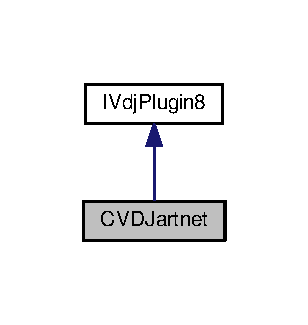
\includegraphics[width=148pt]{classCVDJartnet__inherit__graph}
\end{center}
\end{figure}


Collaboration diagram for C\+V\+D\+Jartnet\+:
\nopagebreak
\begin{figure}[H]
\begin{center}
\leavevmode
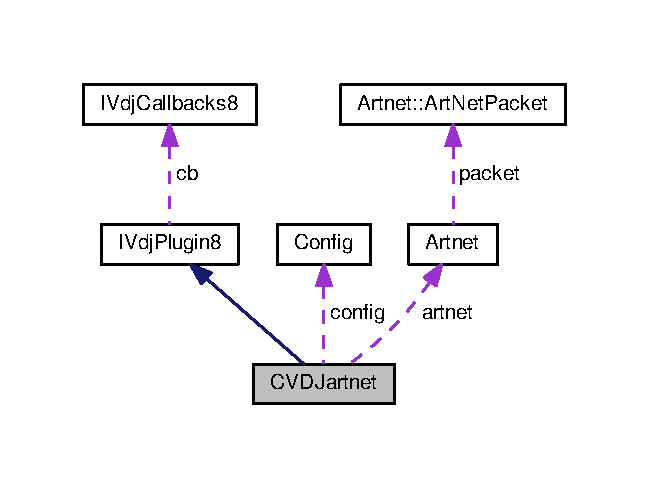
\includegraphics[width=312pt]{classCVDJartnet__coll__graph}
\end{center}
\end{figure}
\subsection*{Public Types}
\begin{DoxyCompactItemize}
\item 
\mbox{\Hypertarget{classCVDJartnet_a21c2dd92432ebdc24fdfe9d6f4fdb304}\label{classCVDJartnet_a21c2dd92432ebdc24fdfe9d6f4fdb304}} 
enum \hyperlink{classCVDJartnet_a21c2dd92432ebdc24fdfe9d6f4fdb304}{\+\_\+\+I\+D\+\_\+\+Interface} \{ \newline
{\bfseries I\+D\+\_\+\+E\+N\+A\+B\+L\+E\+\_\+\+B\+U\+T\+T\+ON}, 
{\bfseries I\+D\+\_\+\+R\+E\+F\+R\+E\+S\+H\+\_\+\+B\+U\+T\+T\+ON}, 
{\bfseries I\+D\+\_\+\+C\+O\+N\+F\+I\+G\+\_\+\+B\+U\+T\+T\+ON}, 
{\bfseries I\+D\+\_\+\+S\+E\+T\+UP}, 
\newline
{\bfseries I\+D\+\_\+\+S\+A\+VE}
 \}\begin{DoxyCompactList}\small\item\em The properties that can be passed to \hyperlink{classCVDJartnet_a7acdd06e91ab522c8a5facddc4a58e43}{On\+Parameter(int id)} \end{DoxyCompactList}
\item 
\mbox{\Hypertarget{classCVDJartnet_a932dbf4dc412424e9349a298ee1f4363}\label{classCVDJartnet_a932dbf4dc412424e9349a298ee1f4363}} 
typedef enum \hyperlink{classCVDJartnet_a21c2dd92432ebdc24fdfe9d6f4fdb304}{C\+V\+D\+Jartnet\+::\+\_\+\+I\+D\+\_\+\+Interface} \hyperlink{classCVDJartnet_a932dbf4dc412424e9349a298ee1f4363}{I\+D\+\_\+\+Interface}
\begin{DoxyCompactList}\small\item\em The properties that can be passed to \hyperlink{classCVDJartnet_a7acdd06e91ab522c8a5facddc4a58e43}{On\+Parameter(int id)} \end{DoxyCompactList}\end{DoxyCompactItemize}
\subsection*{Public Member Functions}
\begin{DoxyCompactItemize}
\item 
H\+R\+E\+S\+U\+LT V\+D\+J\+\_\+\+A\+PI \hyperlink{classCVDJartnet_aad029c72cf6bcb2baae197124a1d5493}{On\+Load} ()
\begin{DoxyCompactList}\small\item\em The config has been loaded by Virtual\+DJ. \end{DoxyCompactList}\item 
\mbox{\Hypertarget{classCVDJartnet_a16aaaf2b400ca3a0489b7504ef4380f2}\label{classCVDJartnet_a16aaaf2b400ca3a0489b7504ef4380f2}} 
H\+R\+E\+S\+U\+LT V\+D\+J\+\_\+\+A\+PI \hyperlink{classCVDJartnet_a16aaaf2b400ca3a0489b7504ef4380f2}{On\+Get\+Plugin\+Info} (\hyperlink{structTVdjPluginInfo8}{T\+Vdj\+Plugin\+Info8} $\ast$infos)
\begin{DoxyCompactList}\small\item\em Give the plugin info to Virtual\+DJ. \end{DoxyCompactList}\item 
\mbox{\Hypertarget{classCVDJartnet_a26fc17b4324977c96db0875c2c9510b0}\label{classCVDJartnet_a26fc17b4324977c96db0875c2c9510b0}} 
U\+L\+O\+NG V\+D\+J\+\_\+\+A\+PI \hyperlink{classCVDJartnet_a26fc17b4324977c96db0875c2c9510b0}{Release} ()
\begin{DoxyCompactList}\small\item\em Release the plugin memory. \end{DoxyCompactList}\item 
\mbox{\Hypertarget{classCVDJartnet_ab773cdddc551d8db370ef756405a4412}\label{classCVDJartnet_ab773cdddc551d8db370ef756405a4412}} 
H\+R\+E\+S\+U\+LT V\+D\+J\+\_\+\+A\+PI \hyperlink{classCVDJartnet_ab773cdddc551d8db370ef756405a4412}{On\+Get\+User\+Interface} (\hyperlink{structTVdjPluginInterface8}{T\+Vdj\+Plugin\+Interface8} $\ast$plugin\+Interface)
\begin{DoxyCompactList}\small\item\em Give the plugin interface to Virtual\+DJ. \end{DoxyCompactList}\item 
\mbox{\Hypertarget{classCVDJartnet_a7acdd06e91ab522c8a5facddc4a58e43}\label{classCVDJartnet_a7acdd06e91ab522c8a5facddc4a58e43}} 
H\+R\+E\+S\+U\+LT V\+D\+J\+\_\+\+A\+PI \hyperlink{classCVDJartnet_a7acdd06e91ab522c8a5facddc4a58e43}{On\+Parameter} (int id)
\begin{DoxyCompactList}\small\item\em A button has been pressed. \end{DoxyCompactList}\item 
\mbox{\Hypertarget{classCVDJartnet_a2b6a30190c13882c67bee402a3069c6a}\label{classCVDJartnet_a2b6a30190c13882c67bee402a3069c6a}} 
H\+R\+E\+S\+U\+LT V\+D\+J\+\_\+\+A\+PI \hyperlink{classCVDJartnet_a2b6a30190c13882c67bee402a3069c6a}{On\+Get\+Parameter\+String} (int id, char $\ast$out\+Param, int out\+Param\+Size)
\begin{DoxyCompactList}\small\item\em Give the property label string to Virtual\+DJ. \end{DoxyCompactList}\item 
\mbox{\Hypertarget{classCVDJartnet_aed57c58c3ca5fe51181244bd745a2d75}\label{classCVDJartnet_aed57c58c3ca5fe51181244bd745a2d75}} 
void \hyperlink{classCVDJartnet_aed57c58c3ca5fe51181244bd745a2d75}{init} ()
\begin{DoxyCompactList}\small\item\em Initialise the plugin once Virtual\+DJ A\+P\+Is can be called. \end{DoxyCompactList}\item 
\mbox{\Hypertarget{classCVDJartnet_a195690a1e5100b728ddf9da7a5d0608d}\label{classCVDJartnet_a195690a1e5100b728ddf9da7a5d0608d}} 
void \hyperlink{classCVDJartnet_a195690a1e5100b728ddf9da7a5d0608d}{update\+D\+M\+Xvalues} ()
\begin{DoxyCompactList}\small\item\em Get the D\+MX values from Virtual\+DJ and send them over Art-\/\+Net. \end{DoxyCompactList}\end{DoxyCompactItemize}
\subsection*{Static Public Member Functions}
\begin{DoxyCompactItemize}
\item 
\mbox{\Hypertarget{classCVDJartnet_a34007cb1abb536fc1c50c54e42c970f8}\label{classCVDJartnet_a34007cb1abb536fc1c50c54e42c970f8}} 
static \hyperlink{classCVDJartnet}{C\+V\+D\+Jartnet} $\ast$ \hyperlink{classCVDJartnet_a34007cb1abb536fc1c50c54e42c970f8}{get\+Instance} ()
\begin{DoxyCompactList}\small\item\em Get the singleton instance of the plugin. \end{DoxyCompactList}\end{DoxyCompactItemize}
\subsection*{Public Attributes}
\begin{DoxyCompactItemize}
\item 
\mbox{\Hypertarget{classCVDJartnet_ae8cb7dd606f4412ccd5c3027945bb6c6}\label{classCVDJartnet_ae8cb7dd606f4412ccd5c3027945bb6c6}} 
int \hyperlink{classCVDJartnet_ae8cb7dd606f4412ccd5c3027945bb6c6}{m\+\_\+\+Enable}
\begin{DoxyCompactList}\small\item\em Whether the plugin is enabled. \end{DoxyCompactList}\item 
\mbox{\Hypertarget{classCVDJartnet_ac441cca0ec16ec5d572a7b34fef7f134}\label{classCVDJartnet_ac441cca0ec16ec5d572a7b34fef7f134}} 
int \hyperlink{classCVDJartnet_ac441cca0ec16ec5d572a7b34fef7f134}{m\+\_\+\+Refresh}
\begin{DoxyCompactList}\small\item\em Reload the config data. \end{DoxyCompactList}\item 
\mbox{\Hypertarget{classCVDJartnet_a686ac746d631a668272ad5f87b2f4db2}\label{classCVDJartnet_a686ac746d631a668272ad5f87b2f4db2}} 
int \hyperlink{classCVDJartnet_a686ac746d631a668272ad5f87b2f4db2}{m\+\_\+\+Config}
\begin{DoxyCompactList}\small\item\em Open the config tool. \end{DoxyCompactList}\item 
\mbox{\Hypertarget{classCVDJartnet_a817d2020541e2af6e0833a061d352fae}\label{classCVDJartnet_a817d2020541e2af6e0833a061d352fae}} 
\hyperlink{classConfig}{Config} $\ast$ \hyperlink{classCVDJartnet_a817d2020541e2af6e0833a061d352fae}{config}
\begin{DoxyCompactList}\small\item\em The config parser. \end{DoxyCompactList}\item 
void $\ast$ \hyperlink{classCVDJartnet_ab24b02521183e5d8cf6884e64b3b6e27}{config\+Tool}
\begin{DoxyCompactList}\small\item\em A pointer to the config tool. \end{DoxyCompactList}\end{DoxyCompactItemize}
\subsection*{Static Private Member Functions}
\begin{DoxyCompactItemize}
\item 
\mbox{\Hypertarget{classCVDJartnet_a2bcd778bf57ec099afef11019b72edec}\label{classCVDJartnet_a2bcd778bf57ec099afef11019b72edec}} 
static void \hyperlink{classCVDJartnet_a2bcd778bf57ec099afef11019b72edec}{setup} ()
\begin{DoxyCompactList}\small\item\em Setup the singleton instance of the plugin. \end{DoxyCompactList}\item 
\mbox{\Hypertarget{classCVDJartnet_ad637fadb322107a12528154198157fcc}\label{classCVDJartnet_ad637fadb322107a12528154198157fcc}} 
static void \hyperlink{classCVDJartnet_ad637fadb322107a12528154198157fcc}{update} ()
\begin{DoxyCompactList}\small\item\em Poll Virtual\+DJ and send the data over Art-\/\+Net. \end{DoxyCompactList}\end{DoxyCompactItemize}
\subsection*{Private Attributes}
\begin{DoxyCompactItemize}
\item 
\mbox{\Hypertarget{classCVDJartnet_a1cbe7b41ac0c19c24743d23e377888c1}\label{classCVDJartnet_a1cbe7b41ac0c19c24743d23e377888c1}} 
\hyperlink{classArtnet}{Artnet} \hyperlink{classCVDJartnet_a1cbe7b41ac0c19c24743d23e377888c1}{artnet}
\begin{DoxyCompactList}\small\item\em The object that sends the Art-\/\+Net data. \end{DoxyCompactList}\item 
\mbox{\Hypertarget{classCVDJartnet_a61ed7725b775d516e9f34e3ed9113d62}\label{classCVDJartnet_a61ed7725b775d516e9f34e3ed9113d62}} 
int \hyperlink{classCVDJartnet_a61ed7725b775d516e9f34e3ed9113d62}{skipped\+Packets} = 0
\begin{DoxyCompactList}\small\item\em The number of packets that have been skipped since the last sent packet. \end{DoxyCompactList}\item 
\mbox{\Hypertarget{classCVDJartnet_abbc42ef43456cdbd170ed46118fced1b}\label{classCVDJartnet_abbc42ef43456cdbd170ed46118fced1b}} 
int \hyperlink{classCVDJartnet_abbc42ef43456cdbd170ed46118fced1b}{skip\+Packet\+Limit} = 10
\begin{DoxyCompactList}\small\item\em The maximum number of packets that can be skipped before one is sent. \end{DoxyCompactList}\item 
void $\ast$ \hyperlink{classCVDJartnet_ae1b2c37bca6832820d7a6cd9df718d02}{setup\+Thread}
\begin{DoxyCompactList}\small\item\em The thread used to initialise the plugin. \end{DoxyCompactList}\item 
void $\ast$ \hyperlink{classCVDJartnet_adef23f780e10ff58e5b24aedde084489}{poll\+Thread}
\begin{DoxyCompactList}\small\item\em The thread used to poll Virtual\+DJ and send the data over Art-\/\+Net. \end{DoxyCompactList}\end{DoxyCompactItemize}


\subsection{Detailed Description}
A singleton class representing the plugin. 

\subsection{Member Function Documentation}
\mbox{\Hypertarget{classCVDJartnet_aad029c72cf6bcb2baae197124a1d5493}\label{classCVDJartnet_aad029c72cf6bcb2baae197124a1d5493}} 
\index{C\+V\+D\+Jartnet@{C\+V\+D\+Jartnet}!On\+Load@{On\+Load}}
\index{On\+Load@{On\+Load}!C\+V\+D\+Jartnet@{C\+V\+D\+Jartnet}}
\subsubsection{\texorpdfstring{On\+Load()}{OnLoad()}}
{\footnotesize\ttfamily H\+R\+E\+S\+U\+LT V\+D\+J\+\_\+\+A\+PI C\+V\+D\+Jartnet\+::\+On\+Load (\begin{DoxyParamCaption}{ }\end{DoxyParamCaption})\hspace{0.3cm}{\ttfamily [virtual]}}



The config has been loaded by Virtual\+DJ. 

Virtual\+DJ A\+P\+Is cannot be called from this function 

Reimplemented from \hyperlink{classIVdjPlugin8}{I\+Vdj\+Plugin8}.



\subsection{Member Data Documentation}
\mbox{\Hypertarget{classCVDJartnet_ab24b02521183e5d8cf6884e64b3b6e27}\label{classCVDJartnet_ab24b02521183e5d8cf6884e64b3b6e27}} 
\index{C\+V\+D\+Jartnet@{C\+V\+D\+Jartnet}!config\+Tool@{config\+Tool}}
\index{config\+Tool@{config\+Tool}!C\+V\+D\+Jartnet@{C\+V\+D\+Jartnet}}
\subsubsection{\texorpdfstring{config\+Tool}{configTool}}
{\footnotesize\ttfamily void$\ast$ C\+V\+D\+Jartnet\+::config\+Tool}



A pointer to the config tool. 

This is a void$\ast$ because on different platforms the type is different. \mbox{\Hypertarget{classCVDJartnet_adef23f780e10ff58e5b24aedde084489}\label{classCVDJartnet_adef23f780e10ff58e5b24aedde084489}} 
\index{C\+V\+D\+Jartnet@{C\+V\+D\+Jartnet}!poll\+Thread@{poll\+Thread}}
\index{poll\+Thread@{poll\+Thread}!C\+V\+D\+Jartnet@{C\+V\+D\+Jartnet}}
\subsubsection{\texorpdfstring{poll\+Thread}{pollThread}}
{\footnotesize\ttfamily void$\ast$ C\+V\+D\+Jartnet\+::poll\+Thread\hspace{0.3cm}{\ttfamily [private]}}



The thread used to poll Virtual\+DJ and send the data over Art-\/\+Net. 

Of type std\+::thread$\ast$ but can\textquotesingle{}t be of thread type as thread is incompatible with C\+LR. \mbox{\Hypertarget{classCVDJartnet_ae1b2c37bca6832820d7a6cd9df718d02}\label{classCVDJartnet_ae1b2c37bca6832820d7a6cd9df718d02}} 
\index{C\+V\+D\+Jartnet@{C\+V\+D\+Jartnet}!setup\+Thread@{setup\+Thread}}
\index{setup\+Thread@{setup\+Thread}!C\+V\+D\+Jartnet@{C\+V\+D\+Jartnet}}
\subsubsection{\texorpdfstring{setup\+Thread}{setupThread}}
{\footnotesize\ttfamily void$\ast$ C\+V\+D\+Jartnet\+::setup\+Thread\hspace{0.3cm}{\ttfamily [private]}}



The thread used to initialise the plugin. 

Of type std\+::thread$\ast$ but can\textquotesingle{}t be of thread type as thread is incompatible with C\+LR. 

The documentation for this class was generated from the following files\+:\begin{DoxyCompactItemize}
\item 
src/V\+D\+Jartnet.\+hpp\item 
src/V\+D\+Jartnet.\+cpp\end{DoxyCompactItemize}

\hypertarget{structIConfigWinTableView}{}\section{I\+Config\+Win\+Table\+View Struct Reference}
\label{structIConfigWinTableView}\index{I\+Config\+Win\+Table\+View@{I\+Config\+Win\+Table\+View}}


Inheritance diagram for I\+Config\+Win\+Table\+View\+:
\nopagebreak
\begin{figure}[H]
\begin{center}
\leavevmode
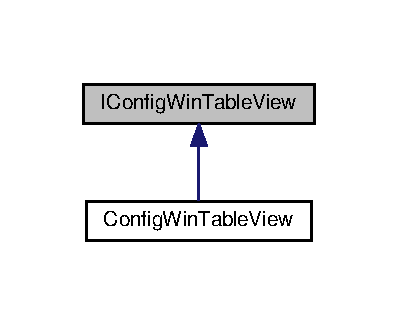
\includegraphics[width=191pt]{structIConfigWinTableView__inherit__graph}
\end{center}
\end{figure}
\subsection*{Events}
\begin{DoxyCompactItemize}
\item 
\mbox{\Hypertarget{structIConfigWinTableView_a876cbf8e536ccf34a7dda3b45b156362}\label{structIConfigWinTableView_a876cbf8e536ccf34a7dda3b45b156362}} 
Config\+Win\+Table\+View\+Key\+Event\+Handler$^\wedge$ {\bfseries Config\+Table\+View\+Key\+Down}
\end{DoxyCompactItemize}


The documentation for this struct was generated from the following file\+:\begin{DoxyCompactItemize}
\item 
src/Config\+Win\+Table\+View.\+hpp\end{DoxyCompactItemize}

\hypertarget{structIVdjCallbacks8}{}\section{I\+Vdj\+Callbacks8 Struct Reference}
\label{structIVdjCallbacks8}\index{I\+Vdj\+Callbacks8@{I\+Vdj\+Callbacks8}}
\subsection*{Public Member Functions}
\begin{DoxyCompactItemize}
\item 
\mbox{\Hypertarget{structIVdjCallbacks8_a82e20361953da177f739ed6cf55b47ed}\label{structIVdjCallbacks8_a82e20361953da177f739ed6cf55b47ed}} 
virtual H\+R\+E\+S\+U\+LT {\bfseries Send\+Command} (const char $\ast$command)=0
\item 
\mbox{\Hypertarget{structIVdjCallbacks8_a73e317136b0fb53187c2bc41b7845403}\label{structIVdjCallbacks8_a73e317136b0fb53187c2bc41b7845403}} 
virtual H\+R\+E\+S\+U\+LT {\bfseries Get\+Info} (const char $\ast$command, double $\ast$result)=0
\item 
\mbox{\Hypertarget{structIVdjCallbacks8_a1136c2b7dcc7ce42a9f67d741cb37bcb}\label{structIVdjCallbacks8_a1136c2b7dcc7ce42a9f67d741cb37bcb}} 
virtual H\+R\+E\+S\+U\+LT {\bfseries Get\+String\+Info} (const char $\ast$command, void $\ast$result, int size)=0
\item 
\mbox{\Hypertarget{structIVdjCallbacks8_a5fdc3c99d9efdbaf368ff1146e134a57}\label{structIVdjCallbacks8_a5fdc3c99d9efdbaf368ff1146e134a57}} 
virtual H\+R\+E\+S\+U\+LT {\bfseries Declare\+Parameter} (void $\ast$parameter, int type, int id, const char $\ast$name, const char $\ast$short\+Name, float defaultvalue)=0
\item 
\mbox{\Hypertarget{structIVdjCallbacks8_a1f52f10cf707d4e8946a966e2ab7de8d}\label{structIVdjCallbacks8_a1f52f10cf707d4e8946a966e2ab7de8d}} 
virtual H\+R\+E\+S\+U\+LT {\bfseries Get\+Song\+Buffer} (int pos, int nb, short $\ast$$\ast$buffer)=0
\end{DoxyCompactItemize}


The documentation for this struct was generated from the following file\+:\begin{DoxyCompactItemize}
\item 
src/vdj\+Plugin8.\+h\end{DoxyCompactItemize}

\hypertarget{classIVdjPlugin8}{}\section{I\+Vdj\+Plugin8 Class Reference}
\label{classIVdjPlugin8}\index{I\+Vdj\+Plugin8@{I\+Vdj\+Plugin8}}


Inheritance diagram for I\+Vdj\+Plugin8\+:
\nopagebreak
\begin{figure}[H]
\begin{center}
\leavevmode
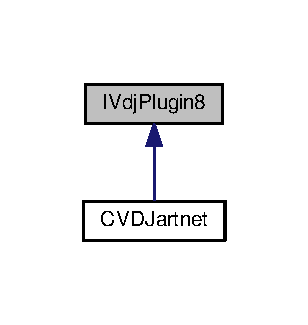
\includegraphics[width=148pt]{classIVdjPlugin8__inherit__graph}
\end{center}
\end{figure}


Collaboration diagram for I\+Vdj\+Plugin8\+:
\nopagebreak
\begin{figure}[H]
\begin{center}
\leavevmode
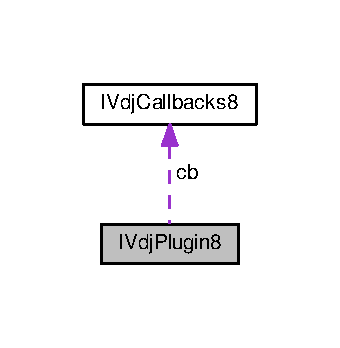
\includegraphics[width=163pt]{classIVdjPlugin8__coll__graph}
\end{center}
\end{figure}
\subsection*{Public Member Functions}
\begin{DoxyCompactItemize}
\item 
\mbox{\Hypertarget{classIVdjPlugin8_a3d8f43115ff34854656ba49ea23cf539}\label{classIVdjPlugin8_a3d8f43115ff34854656ba49ea23cf539}} 
virtual H\+R\+E\+S\+U\+LT V\+D\+J\+\_\+\+A\+PI {\bfseries On\+Load} ()
\item 
\mbox{\Hypertarget{classIVdjPlugin8_a5786b8ff044662a490cd0d357d792aa3}\label{classIVdjPlugin8_a5786b8ff044662a490cd0d357d792aa3}} 
virtual H\+R\+E\+S\+U\+LT V\+D\+J\+\_\+\+A\+PI {\bfseries On\+Get\+Plugin\+Info} (\hyperlink{structTVdjPluginInfo8}{T\+Vdj\+Plugin\+Info8} $\ast$info)
\item 
\mbox{\Hypertarget{classIVdjPlugin8_a244c0f64c417bbf6939b7124e3d02fae}\label{classIVdjPlugin8_a244c0f64c417bbf6939b7124e3d02fae}} 
virtual U\+L\+O\+NG V\+D\+J\+\_\+\+A\+PI {\bfseries Release} ()
\item 
\mbox{\Hypertarget{classIVdjPlugin8_a2bae319b61a5cecb78278983f5efa90d}\label{classIVdjPlugin8_a2bae319b61a5cecb78278983f5efa90d}} 
H\+R\+E\+S\+U\+LT {\bfseries Declare\+Parameter\+Button} (int $\ast$parameter, int id, const char $\ast$name, const char $\ast$short\+Name)
\item 
\mbox{\Hypertarget{classIVdjPlugin8_ac8981776c1c8a27049c4fbf13c6bfb4c}\label{classIVdjPlugin8_ac8981776c1c8a27049c4fbf13c6bfb4c}} 
H\+R\+E\+S\+U\+LT {\bfseries Declare\+Parameter\+Slider} (float $\ast$parameter, int id, const char $\ast$name, const char $\ast$short\+Name, float defaultvalue)
\item 
\mbox{\Hypertarget{classIVdjPlugin8_a24d43202c1ef7f867c64325f0e59abd3}\label{classIVdjPlugin8_a24d43202c1ef7f867c64325f0e59abd3}} 
H\+R\+E\+S\+U\+LT {\bfseries Declare\+Parameter\+Switch} (int $\ast$parameter, int id, const char $\ast$name, const char $\ast$short\+Name, bool defaultvalue)
\item 
\mbox{\Hypertarget{classIVdjPlugin8_a5ec6f3e2448054700f05d0ff15efd007}\label{classIVdjPlugin8_a5ec6f3e2448054700f05d0ff15efd007}} 
H\+R\+E\+S\+U\+LT {\bfseries Declare\+Parameter\+String} (char $\ast$parameter, int id, const char $\ast$name, const char $\ast$short\+Name, int parameter\+Size)
\item 
\mbox{\Hypertarget{classIVdjPlugin8_aa9c38ce43050710f555ee94ccb16de65}\label{classIVdjPlugin8_aa9c38ce43050710f555ee94ccb16de65}} 
H\+R\+E\+S\+U\+LT {\bfseries Declare\+Parameter\+Custom} (void $\ast$parameter, int id, const char $\ast$name, const char $\ast$short\+Name, int parameter\+Size)
\item 
\mbox{\Hypertarget{classIVdjPlugin8_a9b2047ebefc35d7ea4160233de3baf28}\label{classIVdjPlugin8_a9b2047ebefc35d7ea4160233de3baf28}} 
H\+R\+E\+S\+U\+LT {\bfseries Declare\+Parameter\+Radio} (int $\ast$parameter, int id, const char $\ast$name, const char $\ast$short\+Name, float defaultvalue)
\item 
\mbox{\Hypertarget{classIVdjPlugin8_a2b3826b844605723569da77ced2e36ee}\label{classIVdjPlugin8_a2b3826b844605723569da77ced2e36ee}} 
H\+R\+E\+S\+U\+LT {\bfseries Declare\+Parameter\+Command} (char $\ast$parameter, int id, const char $\ast$name, const char $\ast$short\+Name, int parameter\+Size)
\item 
\mbox{\Hypertarget{classIVdjPlugin8_a60e9027c4a583a2cdd739eae3dba0f0d}\label{classIVdjPlugin8_a60e9027c4a583a2cdd739eae3dba0f0d}} 
virtual H\+R\+E\+S\+U\+LT V\+D\+J\+\_\+\+A\+PI {\bfseries On\+Parameter} (int id)
\item 
\mbox{\Hypertarget{classIVdjPlugin8_a5dec0d88ee3d449d0b191e2a36a9837a}\label{classIVdjPlugin8_a5dec0d88ee3d449d0b191e2a36a9837a}} 
virtual H\+R\+E\+S\+U\+LT V\+D\+J\+\_\+\+A\+PI {\bfseries On\+Get\+Parameter\+String} (int id, char $\ast$out\+Param, int out\+Param\+Size)
\item 
\mbox{\Hypertarget{classIVdjPlugin8_a774e79c75ba05e853a0de10242bbee06}\label{classIVdjPlugin8_a774e79c75ba05e853a0de10242bbee06}} 
virtual H\+R\+E\+S\+U\+LT V\+D\+J\+\_\+\+A\+PI {\bfseries On\+Get\+User\+Interface} (\hyperlink{structTVdjPluginInterface8}{T\+Vdj\+Plugin\+Interface8} $\ast$plugin\+Interface)
\item 
\mbox{\Hypertarget{classIVdjPlugin8_a786f7417cdce43e1c5c76c8ca9261f3c}\label{classIVdjPlugin8_a786f7417cdce43e1c5c76c8ca9261f3c}} 
H\+R\+E\+S\+U\+LT {\bfseries Send\+Command} (const char $\ast$command)
\item 
\mbox{\Hypertarget{classIVdjPlugin8_a9edae9daec17cf9f9310f76c1c676537}\label{classIVdjPlugin8_a9edae9daec17cf9f9310f76c1c676537}} 
H\+R\+E\+S\+U\+LT {\bfseries Get\+Info} (const char $\ast$command, double $\ast$result)
\item 
\mbox{\Hypertarget{classIVdjPlugin8_aa4b2ca8146adac0d7f9a7b0dc1bd92e8}\label{classIVdjPlugin8_aa4b2ca8146adac0d7f9a7b0dc1bd92e8}} 
H\+R\+E\+S\+U\+LT {\bfseries Get\+String\+Info} (const char $\ast$command, char $\ast$result, int size)
\end{DoxyCompactItemize}
\subsection*{Public Attributes}
\begin{DoxyCompactItemize}
\item 
\mbox{\Hypertarget{classIVdjPlugin8_a63c6c04d5ded84e16ca23329ed682490}\label{classIVdjPlugin8_a63c6c04d5ded84e16ca23329ed682490}} 
V\+D\+J\+\_\+\+H\+I\+N\+S\+T\+A\+N\+CE {\bfseries h\+Instance}
\item 
\mbox{\Hypertarget{classIVdjPlugin8_a7d7012ae0b26d9700107408c0ec229ed}\label{classIVdjPlugin8_a7d7012ae0b26d9700107408c0ec229ed}} 
\hyperlink{structIVdjCallbacks8}{I\+Vdj\+Callbacks8} $\ast$ {\bfseries cb}
\end{DoxyCompactItemize}


The documentation for this class was generated from the following file\+:\begin{DoxyCompactItemize}
\item 
src/vdj\+Plugin8.\+h\end{DoxyCompactItemize}

\hypertarget{structPreset}{}\section{Preset Struct Reference}
\label{structPreset}\index{Preset@{Preset}}


A preset representing a common entry in the config file.  




{\ttfamily \#include $<$Config.\+hpp$>$}

\subsection*{Public Attributes}
\begin{DoxyCompactItemize}
\item 
\mbox{\Hypertarget{structPreset_a32643ed384b8a95b2a4216b32ce51c47}\label{structPreset_a32643ed384b8a95b2a4216b32ce51c47}} 
std\+::string \hyperlink{structPreset_a32643ed384b8a95b2a4216b32ce51c47}{name}
\begin{DoxyCompactList}\small\item\em The name to be shown in the list of presets. \end{DoxyCompactList}\item 
\mbox{\Hypertarget{structPreset_a70600a05a1f9c8d5ebe87a9f03e483ae}\label{structPreset_a70600a05a1f9c8d5ebe87a9f03e483ae}} 
std\+::string \hyperlink{structPreset_a70600a05a1f9c8d5ebe87a9f03e483ae}{preset}
\begin{DoxyCompactList}\small\item\em The command to be used when the preset is dragged to the config file. \end{DoxyCompactList}\end{DoxyCompactItemize}


\subsection{Detailed Description}
A preset representing a common entry in the config file. 

The documentation for this struct was generated from the following file\+:\begin{DoxyCompactItemize}
\item 
src/\hyperlink{Config_8hpp}{Config.\+hpp}\end{DoxyCompactItemize}

\hypertarget{classSocket}{}\section{Socket Class Reference}
\label{classSocket}\index{Socket@{Socket}}


$<$ A U\+DP socket  




{\ttfamily \#include $<$Socket.\+hpp$>$}

\subsection*{Public Member Functions}
\begin{DoxyCompactItemize}
\item 
\mbox{\Hypertarget{classSocket_ad584e40f858c7c56d84ffadef63f3ab9}\label{classSocket_ad584e40f858c7c56d84ffadef63f3ab9}} 
\hyperlink{classSocket_ad584e40f858c7c56d84ffadef63f3ab9}{Socket} (unsigned int port, int \hyperlink{classSocket_ad962ba2bb1875300c69ff5b4e6a70cd1}{non\+\_\+blocking})
\begin{DoxyCompactList}\small\item\em Construct a socket with the given source port and value of non\+\_\+blocking. \end{DoxyCompactList}\item 
\mbox{\Hypertarget{classSocket_aeac4eb6379a543d38ed88977d3b6630a}\label{classSocket_aeac4eb6379a543d38ed88977d3b6630a}} 
\hyperlink{classSocket_aeac4eb6379a543d38ed88977d3b6630a}{$\sim$\+Socket} ()
\begin{DoxyCompactList}\small\item\em Destruct the socket. \end{DoxyCompactList}\item 
\mbox{\Hypertarget{classSocket_a557ad7665a79556c164e6b30488f70f9}\label{classSocket_a557ad7665a79556c164e6b30488f70f9}} 
void \hyperlink{classSocket_a557ad7665a79556c164e6b30488f70f9}{send} (std\+::string hostS, unsigned short port, const void $\ast$data, int size)
\begin{DoxyCompactList}\small\item\em Send the given data to the given host and port. \end{DoxyCompactList}\end{DoxyCompactItemize}
\subsection*{Private Attributes}
\begin{DoxyCompactItemize}
\item 
\mbox{\Hypertarget{classSocket_a1d1e25e0a7eddecb3473350a1a8c3178}\label{classSocket_a1d1e25e0a7eddecb3473350a1a8c3178}} 
int \hyperlink{classSocket_a1d1e25e0a7eddecb3473350a1a8c3178}{handle}
\begin{DoxyCompactList}\small\item\em The handle to the socket. \end{DoxyCompactList}\item 
\mbox{\Hypertarget{classSocket_ad962ba2bb1875300c69ff5b4e6a70cd1}\label{classSocket_ad962ba2bb1875300c69ff5b4e6a70cd1}} 
int \hyperlink{classSocket_ad962ba2bb1875300c69ff5b4e6a70cd1}{non\+\_\+blocking}
\begin{DoxyCompactList}\small\item\em Whether the socket is blocking. \end{DoxyCompactList}\end{DoxyCompactItemize}


\subsection{Detailed Description}
$<$ A U\+DP socket 

The documentation for this class was generated from the following files\+:\begin{DoxyCompactItemize}
\item 
src/Socket.\+hpp\item 
src/Socket.\+cpp\end{DoxyCompactItemize}

\hypertarget{structTVdjPluginInfo8}{}\section{T\+Vdj\+Plugin\+Info8 Struct Reference}
\label{structTVdjPluginInfo8}\index{T\+Vdj\+Plugin\+Info8@{T\+Vdj\+Plugin\+Info8}}
\subsection*{Public Attributes}
\begin{DoxyCompactItemize}
\item 
\mbox{\Hypertarget{structTVdjPluginInfo8_af7403b3d59f6da967de77f19868359f5}\label{structTVdjPluginInfo8_af7403b3d59f6da967de77f19868359f5}} 
const char $\ast$ {\bfseries Plugin\+Name}
\item 
\mbox{\Hypertarget{structTVdjPluginInfo8_a3be0cc20dfaab62bc6510e8f449a0e6a}\label{structTVdjPluginInfo8_a3be0cc20dfaab62bc6510e8f449a0e6a}} 
const char $\ast$ {\bfseries Author}
\item 
\mbox{\Hypertarget{structTVdjPluginInfo8_a2767a222a128c408edf3fc2bdbd2dcef}\label{structTVdjPluginInfo8_a2767a222a128c408edf3fc2bdbd2dcef}} 
const char $\ast$ {\bfseries Description}
\item 
\mbox{\Hypertarget{structTVdjPluginInfo8_afa7487e56ec5a59847c2d2a6d26b14c7}\label{structTVdjPluginInfo8_afa7487e56ec5a59847c2d2a6d26b14c7}} 
const char $\ast$ {\bfseries Version}
\item 
\mbox{\Hypertarget{structTVdjPluginInfo8_a49d2d881bb18dcc5aad708c284ce5027}\label{structTVdjPluginInfo8_a49d2d881bb18dcc5aad708c284ce5027}} 
V\+D\+J\+\_\+\+B\+I\+T\+M\+AP {\bfseries Bitmap}
\item 
\mbox{\Hypertarget{structTVdjPluginInfo8_ae47053f7b918d945c553f226960bfb6e}\label{structTVdjPluginInfo8_ae47053f7b918d945c553f226960bfb6e}} 
D\+W\+O\+RD {\bfseries Flags}
\end{DoxyCompactItemize}


The documentation for this struct was generated from the following file\+:\begin{DoxyCompactItemize}
\item 
src/vdj\+Plugin8.\+h\end{DoxyCompactItemize}

\hypertarget{structTVdjPluginInterface8}{}\section{T\+Vdj\+Plugin\+Interface8 Struct Reference}
\label{structTVdjPluginInterface8}\index{T\+Vdj\+Plugin\+Interface8@{T\+Vdj\+Plugin\+Interface8}}
\subsection*{Public Attributes}
\begin{DoxyCompactItemize}
\item 
\mbox{\Hypertarget{structTVdjPluginInterface8_a58e11db37bdc4344555b73667bcb4d39}\label{structTVdjPluginInterface8_a58e11db37bdc4344555b73667bcb4d39}} 
D\+W\+O\+RD {\bfseries Type}
\item 
\mbox{\Hypertarget{structTVdjPluginInterface8_ae74d30940f371b9dc052abbecd6f3ca1}\label{structTVdjPluginInterface8_ae74d30940f371b9dc052abbecd6f3ca1}} 
const char $\ast$ {\bfseries Xml}
\item 
\mbox{\Hypertarget{structTVdjPluginInterface8_a439ca76f75e47ea95368e3fdd3f76af0}\label{structTVdjPluginInterface8_a439ca76f75e47ea95368e3fdd3f76af0}} 
void $\ast$ {\bfseries Image\+Buffer}
\item 
\mbox{\Hypertarget{structTVdjPluginInterface8_a3657e0318201799f7766ec4baba95b6b}\label{structTVdjPluginInterface8_a3657e0318201799f7766ec4baba95b6b}} 
int {\bfseries Image\+Size}
\item 
\mbox{\Hypertarget{structTVdjPluginInterface8_ac34246d8ef349c55e342b36facb5fed9}\label{structTVdjPluginInterface8_ac34246d8ef349c55e342b36facb5fed9}} 
V\+D\+J\+\_\+\+W\+I\+N\+D\+OW {\bfseries h\+Wnd}
\end{DoxyCompactItemize}


The documentation for this struct was generated from the following file\+:\begin{DoxyCompactItemize}
\item 
src/vdj\+Plugin8.\+h\end{DoxyCompactItemize}

\hypertarget{classCSUndoManager_1_1UndoItem}{}\section{C\+S\+Undo\+Manager\+:\+:Undo\+Item Class Reference}
\label{classCSUndoManager_1_1UndoItem}\index{C\+S\+Undo\+Manager\+::\+Undo\+Item@{C\+S\+Undo\+Manager\+::\+Undo\+Item}}


An event that can be undone.  




Collaboration diagram for C\+S\+Undo\+Manager\+:\+:Undo\+Item\+:
\nopagebreak
\begin{figure}[H]
\begin{center}
\leavevmode
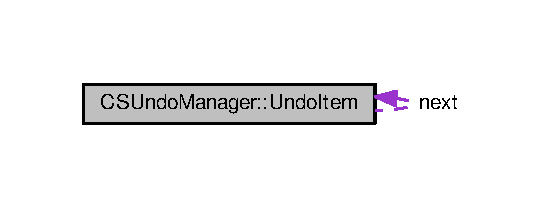
\includegraphics[width=260pt]{classCSUndoManager_1_1UndoItem__coll__graph}
\end{center}
\end{figure}
\subsection*{Public Member Functions}
\begin{DoxyCompactItemize}
\item 
\mbox{\Hypertarget{classCSUndoManager_1_1UndoItem_adddbd4a53854d99d1ad590520d14ba8e}\label{classCSUndoManager_1_1UndoItem_adddbd4a53854d99d1ad590520d14ba8e}} 
\hyperlink{classCSUndoManager_1_1UndoItem_adddbd4a53854d99d1ad590520d14ba8e}{Undo\+Item} (std\+::function$<$ void()$>$ f\+T\+MP, \hyperlink{classCSUndoManager_1_1UndoItem}{Undo\+Item} $\ast$next\+T\+MP)
\begin{DoxyCompactList}\small\item\em Construct an event with the given function and next event. \end{DoxyCompactList}\item 
\mbox{\Hypertarget{classCSUndoManager_1_1UndoItem_a4f1e95e08e088f6890099110474062e3}\label{classCSUndoManager_1_1UndoItem_a4f1e95e08e088f6890099110474062e3}} 
\hyperlink{classCSUndoManager_1_1UndoItem_a4f1e95e08e088f6890099110474062e3}{$\sim$\+Undo\+Item} ()
\begin{DoxyCompactList}\small\item\em Destruct the event and next event. \end{DoxyCompactList}\end{DoxyCompactItemize}
\subsection*{Public Attributes}
\begin{DoxyCompactItemize}
\item 
\mbox{\Hypertarget{classCSUndoManager_1_1UndoItem_aca1eebab67a484cdb8fb4d76d38276b0}\label{classCSUndoManager_1_1UndoItem_aca1eebab67a484cdb8fb4d76d38276b0}} 
std\+::function$<$ void()$>$ \hyperlink{classCSUndoManager_1_1UndoItem_aca1eebab67a484cdb8fb4d76d38276b0}{f}
\begin{DoxyCompactList}\small\item\em The function to be used to undo the event. \end{DoxyCompactList}\item 
\mbox{\Hypertarget{classCSUndoManager_1_1UndoItem_a8619cecf66d3b11ed90e4b1bf91d6026}\label{classCSUndoManager_1_1UndoItem_a8619cecf66d3b11ed90e4b1bf91d6026}} 
\hyperlink{classCSUndoManager_1_1UndoItem}{Undo\+Item} $\ast$ \hyperlink{classCSUndoManager_1_1UndoItem_a8619cecf66d3b11ed90e4b1bf91d6026}{next}
\begin{DoxyCompactList}\small\item\em The next event to undo. \end{DoxyCompactList}\end{DoxyCompactItemize}


\subsection{Detailed Description}
An event that can be undone. 

The documentation for this class was generated from the following file\+:\begin{DoxyCompactItemize}
\item 
src/\+Cpp\+Step/C\+S\+Undo\+Manager.\+hpp\end{DoxyCompactItemize}

\chapter{File Documentation}
\hypertarget{Config_8hpp}{}\section{src/\+Config.hpp File Reference}
\label{Config_8hpp}\index{src/\+Config.\+hpp@{src/\+Config.\+hpp}}
{\ttfamily \#include $<$string$>$}\newline
{\ttfamily \#include $<$vector$>$}\newline
{\ttfamily \#include $<$fstream$>$}\newline
{\ttfamily \#include $<$sstream$>$}\newline
{\ttfamily \#include $<$chrono$>$}\newline
{\ttfamily \#include $<$cmath$>$}\newline
{\ttfamily \#include $<$set$>$}\newline
{\ttfamily \#include $<$iostream$>$}\newline
Include dependency graph for Config.\+hpp\+:
\nopagebreak
\begin{figure}[H]
\begin{center}
\leavevmode
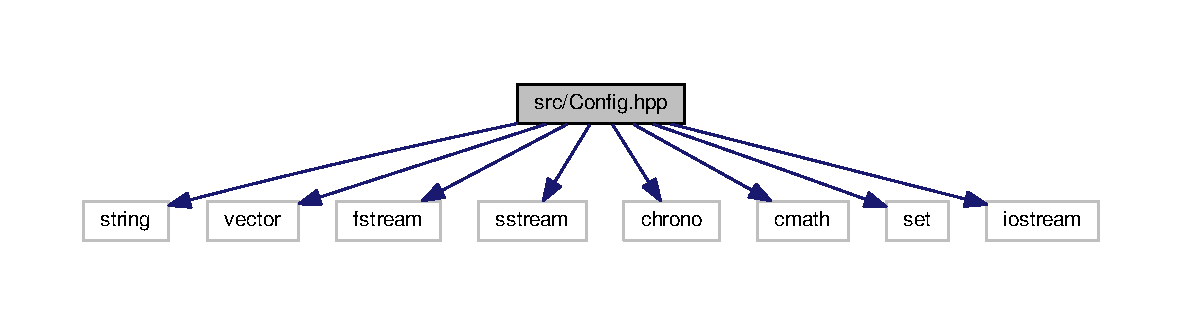
\includegraphics[width=350pt]{Config_8hpp__incl}
\end{center}
\end{figure}
This graph shows which files directly or indirectly include this file\+:
\nopagebreak
\begin{figure}[H]
\begin{center}
\leavevmode
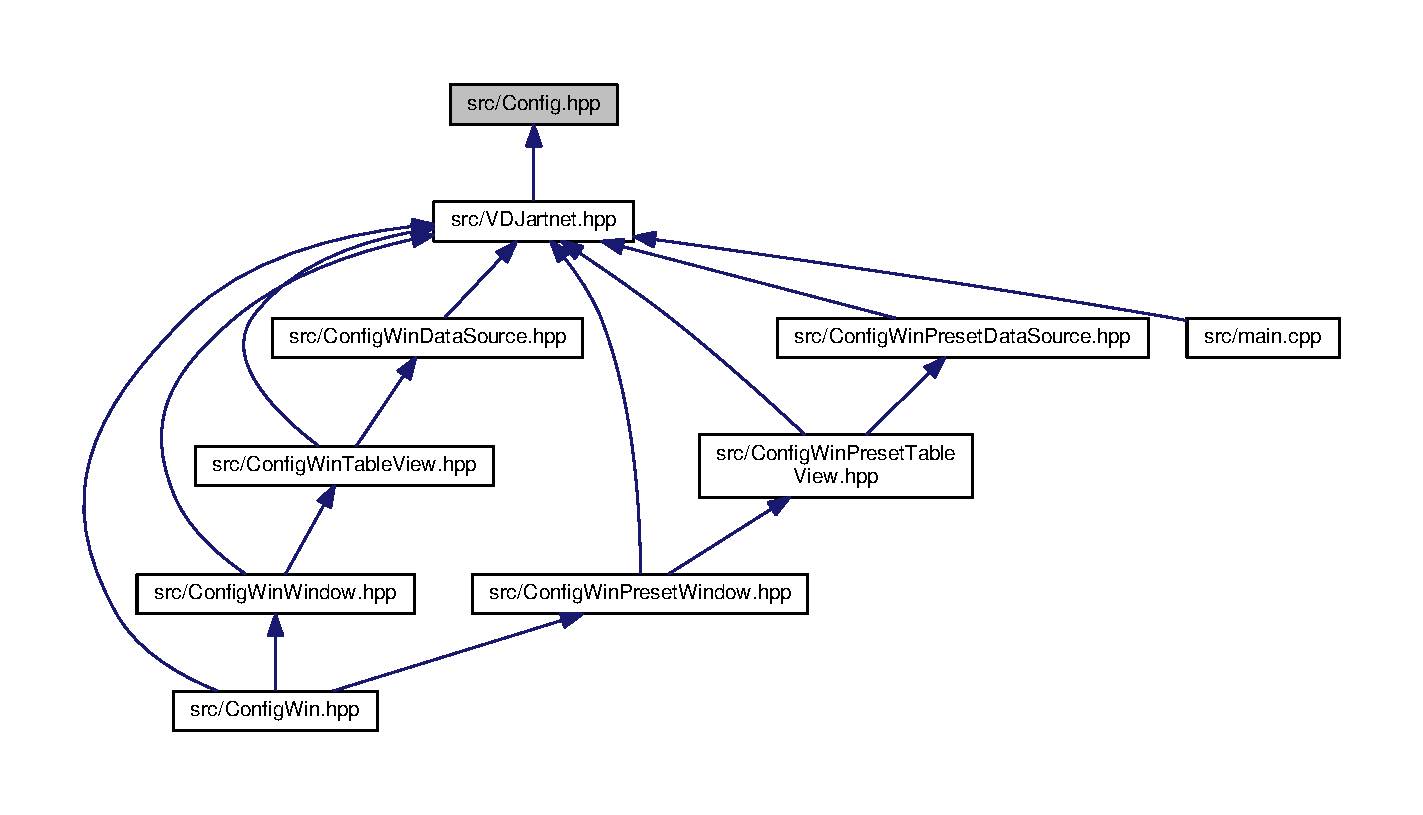
\includegraphics[width=350pt]{Config_8hpp__dep__incl}
\end{center}
\end{figure}
\subsection*{Classes}
\begin{DoxyCompactItemize}
\item 
struct \hyperlink{structPreset}{Preset}
\begin{DoxyCompactList}\small\item\em A preset representing a common entry in the config file. \end{DoxyCompactList}\item 
class \hyperlink{classConfig}{Config}
\begin{DoxyCompactList}\small\item\em A config parser and writer. \end{DoxyCompactList}\end{DoxyCompactItemize}
\subsection*{Functions}
\begin{DoxyCompactItemize}
\item 
\mbox{\Hypertarget{Config_8hpp_a79c612ce8bec9141e246bfb337738a7b}\label{Config_8hpp_a79c612ce8bec9141e246bfb337738a7b}} 
std\+::istream \& \hyperlink{Config_8hpp_a79c612ce8bec9141e246bfb337738a7b}{safe\+Get\+Line} (std\+::istream \&is, std\+::string \&t)
\begin{DoxyCompactList}\small\item\em Get a line from an istream dealing with line endings safely. \end{DoxyCompactList}\end{DoxyCompactItemize}

\hypertarget{ConfigWin_8hpp}{}\section{src/\+Config\+Win.hpp File Reference}
\label{ConfigWin_8hpp}\index{src/\+Config\+Win.\+hpp@{src/\+Config\+Win.\+hpp}}
{\ttfamily \#include \char`\"{}V\+D\+Jartnet.\+hpp\char`\"{}}\newline
{\ttfamily \#include $<$stdio.\+h$>$}\newline
{\ttfamily \#include \char`\"{}Config\+Win\+Window.\+hpp\char`\"{}}\newline
{\ttfamily \#include \char`\"{}Config\+Win\+Preset\+Window.\+hpp\char`\"{}}\newline
{\ttfamily \#include \char`\"{}windows.\+h\char`\"{}}\newline
{\ttfamily \#include $<$msclr\textbackslash{}gcroot.\+h$>$}\newline
Include dependency graph for Config\+Win.\+hpp\+:
\nopagebreak
\begin{figure}[H]
\begin{center}
\leavevmode
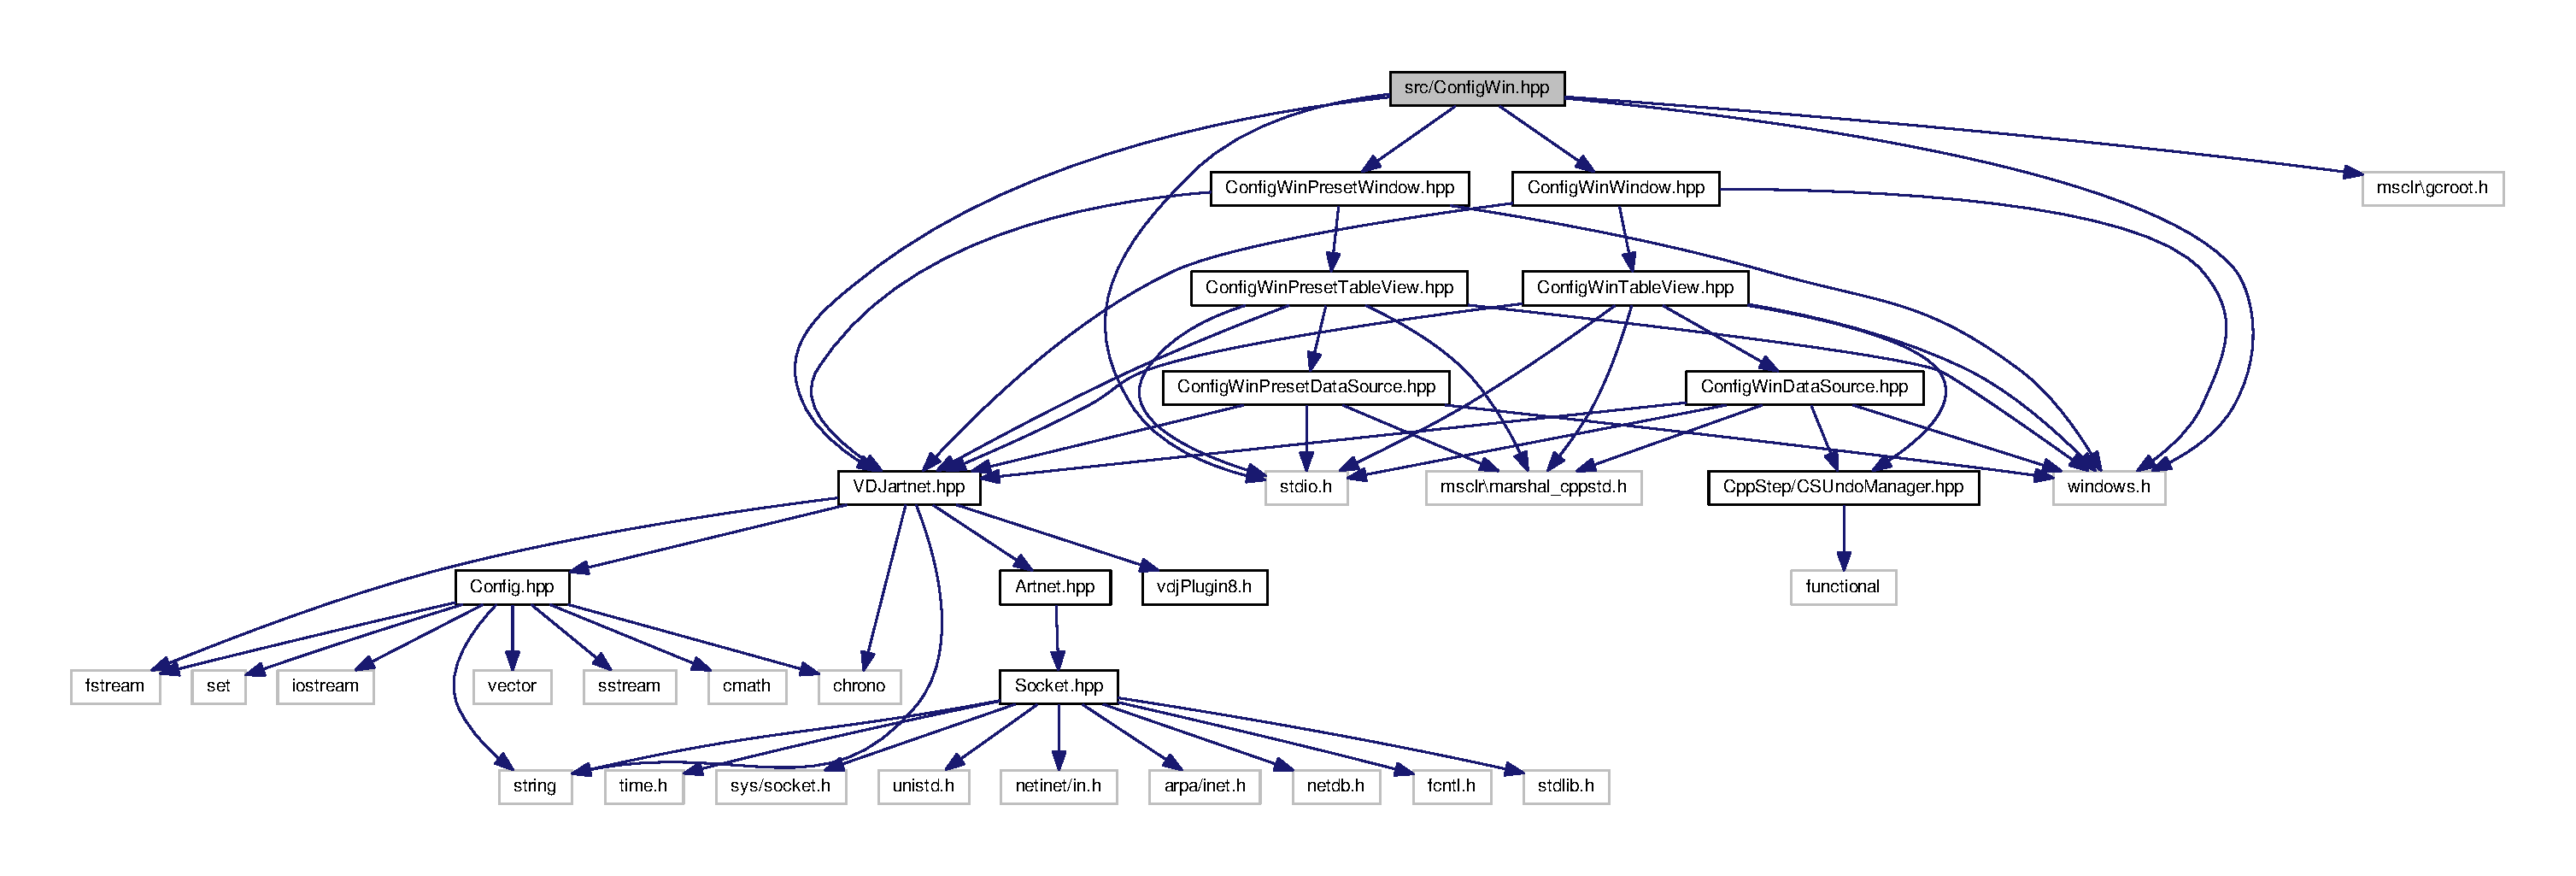
\includegraphics[width=350pt]{ConfigWin_8hpp__incl}
\end{center}
\end{figure}
\subsection*{Classes}
\begin{DoxyCompactItemize}
\item 
class \hyperlink{classConfigWinTool}{Config\+Win\+Tool}
\begin{DoxyCompactList}\small\item\em A config tool to help the user write a correctly formatted config file. \end{DoxyCompactList}\item 
class \hyperlink{classConfigWinToolNative}{Config\+Win\+Tool\+Native}
\begin{DoxyCompactList}\small\item\em An unmanaged wrapper around \hyperlink{classConfigWinTool}{Config\+Win\+Tool}. \end{DoxyCompactList}\end{DoxyCompactItemize}
\subsection*{Functions}
\begin{DoxyCompactItemize}
\item 
\mbox{\Hypertarget{ConfigWin_8hpp_a39d4348bedfc3a884ff9e91f259944d1}\label{ConfigWin_8hpp_a39d4348bedfc3a884ff9e91f259944d1}} 
void $\ast$ \hyperlink{ConfigWin_8hpp_a39d4348bedfc3a884ff9e91f259944d1}{create\+Config\+Win\+Tool} (\hyperlink{classCVDJartnet}{C\+V\+D\+Jartnet} $\ast$vdj\+Artnet)
\begin{DoxyCompactList}\small\item\em Create a config tool with the given instance of the plugin. \end{DoxyCompactList}\item 
\mbox{\Hypertarget{ConfigWin_8hpp_a87b882f96d8655c00527726ebe380044}\label{ConfigWin_8hpp_a87b882f96d8655c00527726ebe380044}} 
void \hyperlink{ConfigWin_8hpp_a87b882f96d8655c00527726ebe380044}{close\+Config\+Win\+Tool} (void $\ast$config\+Window)
\begin{DoxyCompactList}\small\item\em Close the given config tool. \end{DoxyCompactList}\end{DoxyCompactItemize}

\hypertarget{ConfigWinDataSource_8hpp}{}\section{src/\+Config\+Win\+Data\+Source.hpp File Reference}
\label{ConfigWinDataSource_8hpp}\index{src/\+Config\+Win\+Data\+Source.\+hpp@{src/\+Config\+Win\+Data\+Source.\+hpp}}
{\ttfamily \#include $<$stdio.\+h$>$}\newline
{\ttfamily \#include \char`\"{}V\+D\+Jartnet.\+hpp\char`\"{}}\newline
{\ttfamily \#include \char`\"{}Cpp\+Step/\+C\+S\+Undo\+Manager.\+hpp\char`\"{}}\newline
{\ttfamily \#include \char`\"{}windows.\+h\char`\"{}}\newline
{\ttfamily \#include $<$msclr\textbackslash{}marshal\+\_\+cppstd.\+h$>$}\newline
Include dependency graph for Config\+Win\+Data\+Source.\+hpp\+:
\nopagebreak
\begin{figure}[H]
\begin{center}
\leavevmode
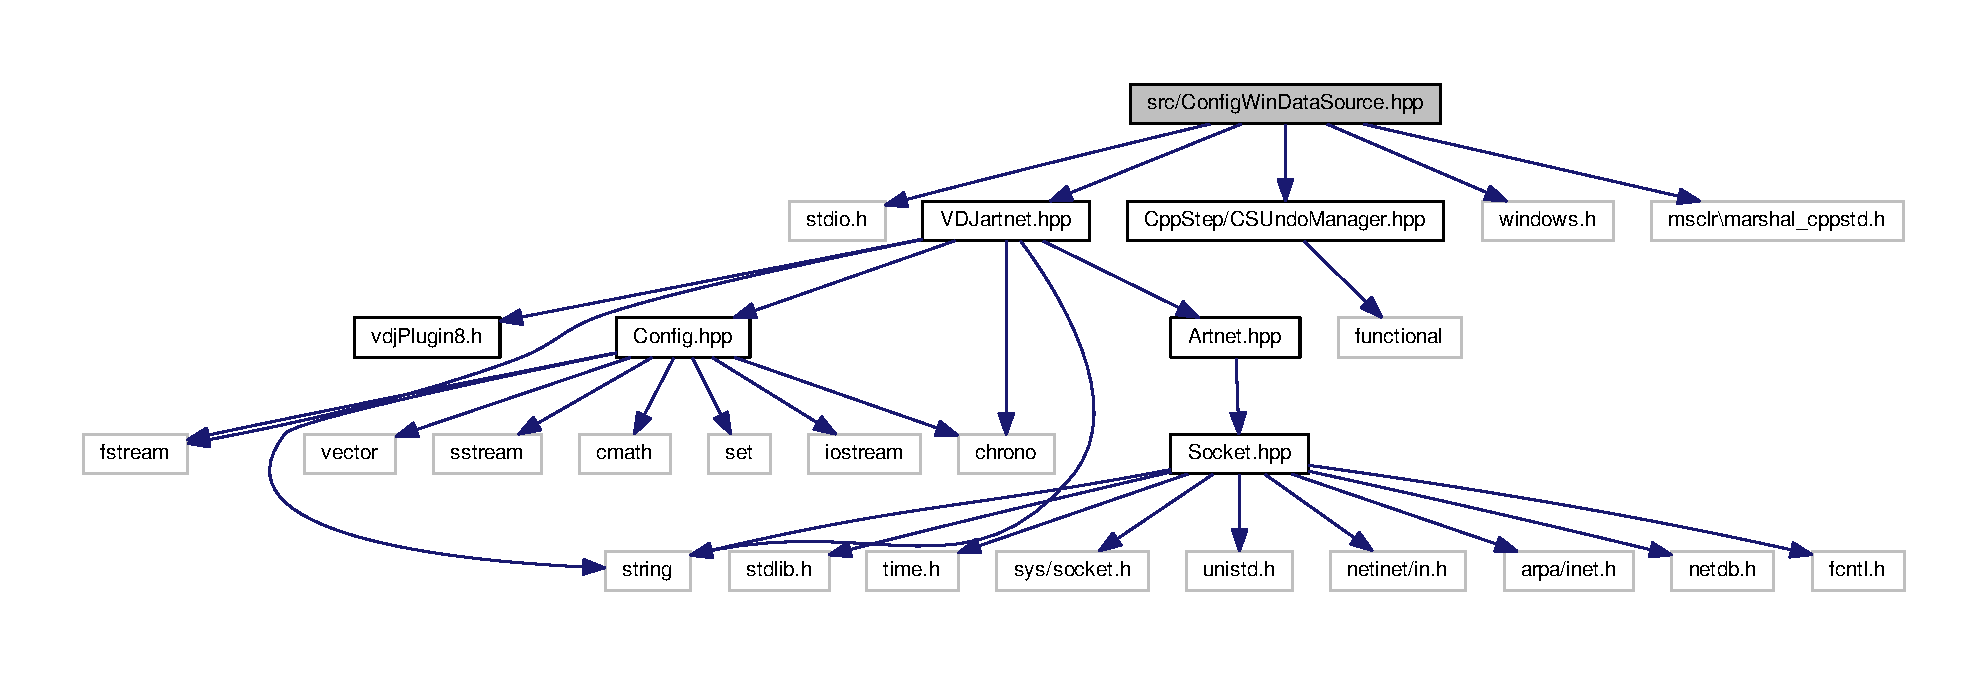
\includegraphics[width=350pt]{ConfigWinDataSource_8hpp__incl}
\end{center}
\end{figure}
This graph shows which files directly or indirectly include this file\+:
\nopagebreak
\begin{figure}[H]
\begin{center}
\leavevmode
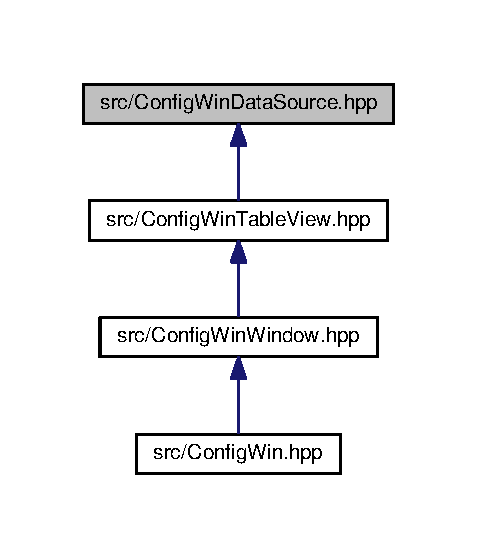
\includegraphics[width=229pt]{ConfigWinDataSource_8hpp__dep__incl}
\end{center}
\end{figure}
\subsection*{Classes}
\begin{DoxyCompactItemize}
\item 
class \hyperlink{classConfigWinRowString}{Config\+Win\+Row\+String}
\begin{DoxyCompactList}\small\item\em A row in the list of commands in the config tool. \end{DoxyCompactList}\end{DoxyCompactItemize}
\subsection*{Typedefs}
\begin{DoxyCompactItemize}
\item 
typedef System\+::\+Collections\+::\+Generic\+::\+List$<$ \hyperlink{classConfigWinRowString}{Config\+Win\+Row\+String}$^\wedge$$>$ \hyperlink{ConfigWinDataSource_8hpp_a78bf2fe0f0a1c6af7fb5dbb43683e579}{Config\+Win\+Data\+Source}
\begin{DoxyCompactList}\small\item\em The data source which shall provide the config rows. \end{DoxyCompactList}\end{DoxyCompactItemize}
\subsection*{Functions}
\begin{DoxyCompactItemize}
\item 
\mbox{\Hypertarget{ConfigWinDataSource_8hpp_aa2b21c9fde56093bf6808c8373d695f9}\label{ConfigWinDataSource_8hpp_aa2b21c9fde56093bf6808c8373d695f9}} 
void \hyperlink{ConfigWinDataSource_8hpp_aa2b21c9fde56093bf6808c8373d695f9}{set\+Value} (gcroot$<$ \hyperlink{classConfigWinRowString}{Config\+Win\+Row\+String}$^\wedge$ const $>$ const target, gcroot$<$ String$^\wedge$ const $>$ const new\+Val)
\begin{DoxyCompactList}\small\item\em Set the value of a given row to a certain value in a native compatible way. \end{DoxyCompactList}\end{DoxyCompactItemize}


\subsection{Typedef Documentation}
\mbox{\Hypertarget{ConfigWinDataSource_8hpp_a78bf2fe0f0a1c6af7fb5dbb43683e579}\label{ConfigWinDataSource_8hpp_a78bf2fe0f0a1c6af7fb5dbb43683e579}} 
\index{Config\+Win\+Data\+Source.\+hpp@{Config\+Win\+Data\+Source.\+hpp}!Config\+Win\+Data\+Source@{Config\+Win\+Data\+Source}}
\index{Config\+Win\+Data\+Source@{Config\+Win\+Data\+Source}!Config\+Win\+Data\+Source.\+hpp@{Config\+Win\+Data\+Source.\+hpp}}
\subsubsection{\texorpdfstring{Config\+Win\+Data\+Source}{ConfigWinDataSource}}
{\footnotesize\ttfamily typedef System\+::\+Collections\+::\+Generic\+::\+List$<$\hyperlink{classConfigWinRowString}{Config\+Win\+Row\+String}$^\wedge$$>$ \hyperlink{ConfigWinDataSource_8hpp_a78bf2fe0f0a1c6af7fb5dbb43683e579}{Config\+Win\+Data\+Source}}



The data source which shall provide the config rows. 

It is a list of the Config\+Win\+Row\+Strings. 
\hypertarget{main_8cpp}{}\section{src/main.cpp File Reference}
\label{main_8cpp}\index{src/main.\+cpp@{src/main.\+cpp}}
{\ttfamily \#include \char`\"{}V\+D\+Jartnet.\+hpp\char`\"{}}\newline
Include dependency graph for main.\+cpp\+:
\nopagebreak
\begin{figure}[H]
\begin{center}
\leavevmode
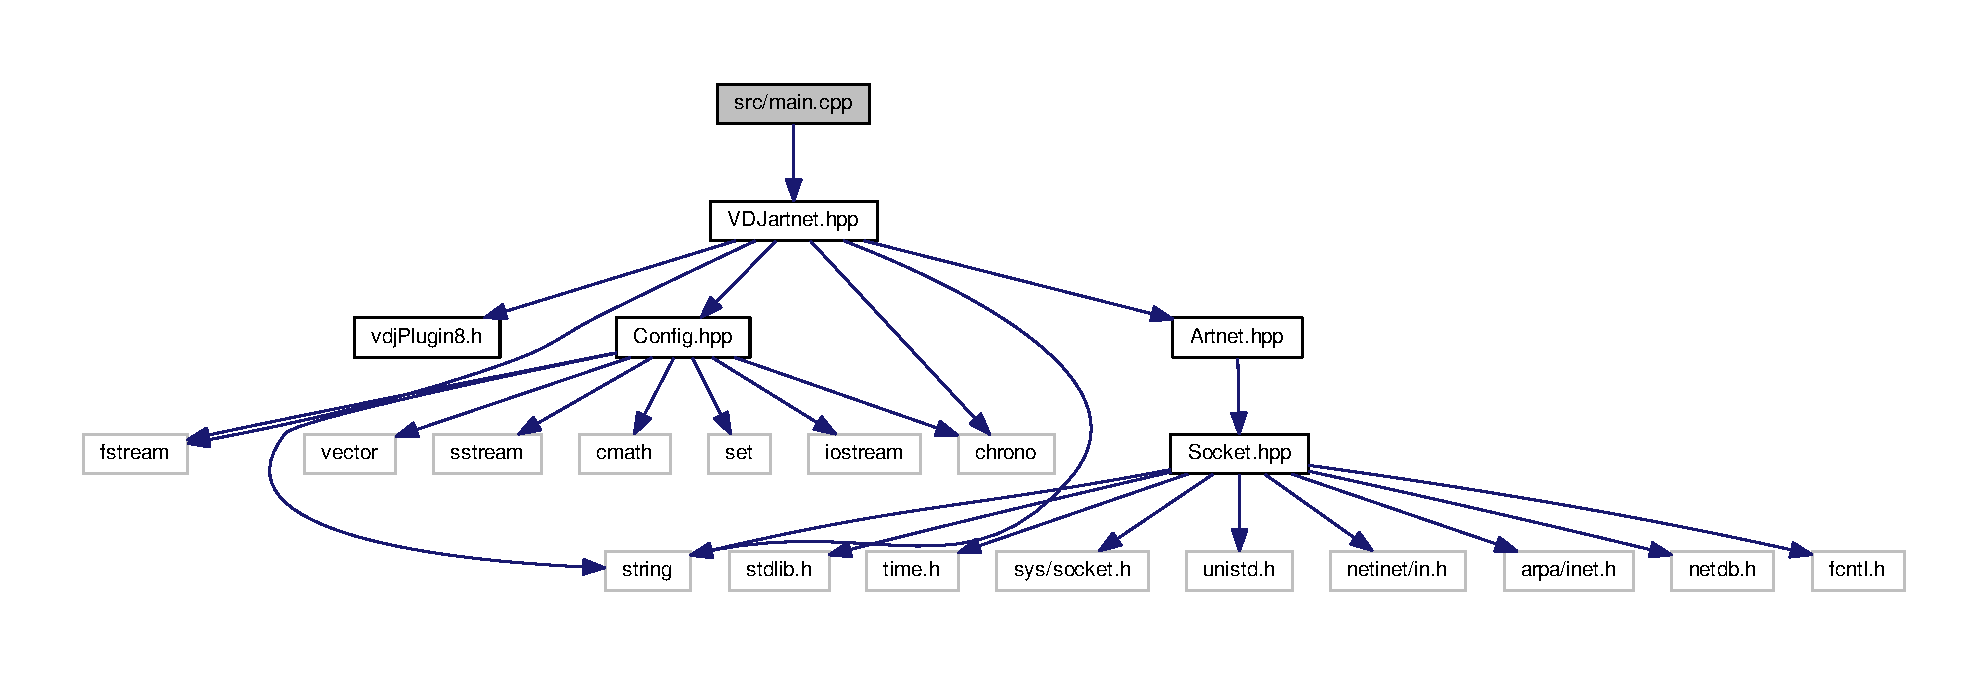
\includegraphics[width=350pt]{main_8cpp__incl}
\end{center}
\end{figure}
\subsection*{Functions}
\begin{DoxyCompactItemize}
\item 
\mbox{\Hypertarget{main_8cpp_a2460da74691b5bc02e70616dccf67a68}\label{main_8cpp_a2460da74691b5bc02e70616dccf67a68}} 
H\+R\+E\+S\+U\+LT V\+D\+J\+\_\+\+A\+PI \hyperlink{main_8cpp_a2460da74691b5bc02e70616dccf67a68}{Dll\+Get\+Class\+Object} (const G\+U\+ID \&rclsid, const G\+U\+ID \&riid, void $\ast$$\ast$pp\+Object)
\begin{DoxyCompactList}\small\item\em Get the singleton instance of the plugin and give it to Virtual\+DJ. \end{DoxyCompactList}\end{DoxyCompactItemize}

%--- End generated contents ---

% Index
\backmatter
\newpage
\phantomsection
\clearemptydoublepage
\addcontentsline{toc}{chapter}{Index}
\printindex

\end{document}
